\documentclass{wileySix}

\usepackage{color}


\usepackage{multirow}
\usepackage{rotating}
\usepackage{amsmath, amssymb}
\usepackage{algorithmic}
\usepackage{algorithm}
\usepackage{graphicx}
\usepackage{subfigure}
\usepackage{epsfig}
\usepackage{balance}
\usepackage{epstopdf}


\hyphenpenalty=5000
\tolerance=1000
\usepackage{float}
\floatstyle{ruled}
\newfloat{algo}{thp}{lop}
\floatname{algo}{Algorithm}
\newcommand{\josh}[1]{}%{{\bf [JOSH:{\em {#1}}]}}
\newcommand{\seyda}[1]{}%{{\bf [SEYDA:{\em {#1}}]}}

\newcommand {\drop}[1] {}
\setcounter{chapter}{6}


\begin{document}

\offprintinfo{Imbalanced Learning: Foundations, Algorithms, and Applications}{Haibo He and Yunqian Ma}

\chapter{Class Imbalance and Active Learning}
\chapterauthors{ Josh Attenberg$^\ast$ and \c{S}eyda Ertekin$^\dag$
\chapteraffil{$^\ast$Etsy; $\dag$Massachusetts Institute of Technology}
}
%	Josh Attenberg \\
%	Etsy \\
%	Brooklyn, NY 11201\\
%	\small\href{mailto:jattenberg@etsy.com}{\nolinkurl{jattenberg@etsy.com}}
%	\and
%	\c{S}eyda Ertekin \\
%	MIT Sloan School of Management \\
%    	Massachusetts Institute of Technology\\
%	Cambridge, MA 02142\\
%	\small\href{mailto:seyda@mit.edu}{\nolinkurl{seyda@mit.edu}}
%	}
\date{}

\noindent\textbf{Abstract}

The performance of a predictive model is tightly coupled with the set of data used in the training process. 
While having more examples available when training will often result in a better informed, more accurate model, 
memory limitations and real-world costs associated with gathering labeled examples often constrain just how 
many training data are available to be considered by a model's training process. In the setting where a only a limited
amount of training data is available during model induction, it often becomes meaninful to consider just which examples
are selected. In {\em Active learning}, the model itself places a hands-on role in the selection of examples for 
labeling, those examples to be used for training. Numerous studies have demonstrated emperically and
theoretically the benefits of active learning.; a training system that interactively involves the model being
trained can often result in a much more accurate model than simply selecting random examples for training, 
given a fixed budget.  Imbalanced settings provide special opportunities and challenges for active learning; 
while active learning can be used to build models that counteractact the harmful effects of learning under class
imbalance, extreme class imbalance can cause an active learning strategy to ``fail'', preventing the selection
scheme from choosing any useful examples for labeling. This chapter focuses on the interaction between actinve
learning and class imbalance, discussing i) active learning techniques designed specifically for dealing with 
imbalanced settings, ii) strategies that leverage active leaning to overcome the deleterious effects of class imbalance, 
iii) how extreme class imbalance can prevent active leaning systems from selecting useful examples, and alternatives
to active learning in these cases. 


\section{Introduction}
\label{sec:intro}

The rich history of predictive modeling has culminated in a diverse set of techniques capable of making accurate predictions on many real-world problems. Many of these techniques demand \emph{training}, whereby a set of instances with ground-truth \emph{labels} (values of a dependent variable) are observed by a model-building process that attempts to capture, at least in part, the relationship between the features of the instances and their labels.  The resultant model can be applied to instances for which the label is not known, to estimate or predict the labels.  These predictions depend not only on the functional structure of the model itself, but on the particular data with which the model was trained.  The accuracy of the predicted labels depends highly on the model's ability to capture an unbiased and sufficient understanding of the characteristics of different classes; in problems where the prevalence of classes is imbalanced, it is necessary to prevent the resultant model from being skewed towards the majority class and to ensure that the model is capable of reflecting the true nature of the minority class.

Another consequence of class imbalance is observed in domains where the ground truth labels in the dataset are not available beforehand and need to be gathered on-demand at some cost.  The costs associated with collecting labels may be due to human labor or as a result of costly incentives, interventions or experiments.  In these settings, simply labeling all available instances may not be practicable, due to budgetary constraints or simply a strong desire to be cost efficient. In a similar fashion to predictive modeling with imbalanced classes, the goal here is to ensure that the budget is not predominantly expended on getting the labels of the majority class instances, and to make sure that the set of instances to be labeled have comparable number of minority class instances as well.

\drop{
In many applications, acquiring a label for a particular instance comes at some cost.  For example, one may employ human labor to ``manually'' examine the instance and record the value of its target variable, often called its label.  In other applications, costly incentives, interventions or experiments may reveal labels.  In such cases, simply labeling all available instances may not be practicable, due to budgetary constraints or simply a strong desire to be cost efficient. The dependence of a model's predictive performance on the selection of data suggests that care should be taken.

The importance of selective label acquisition is evidenced by the vast number of research papers on \emph{active learning}---where the model learned ``so far'' is used in the selection of subsequent data for labeling. This body of research has demonstrated substantial improvements in model generalization performance at a given label budget over a variety of  domains. %However, despite these successes, settings exhibiting strong class imbalance continue to pose a difficult challenge for standard active learning techniques. The intent of this chapter is to provide the reader with some background on these challenges (Section~\ref{sec:background}), detail active learning approaches designed to provide meaningful selections, even when the classes being considered are imbalanced (Sections~\ref{sec:foo} and~\ref{sec:bar}), and to illustrate alternatives to traditional active learning that may be considered when dealing with the most difficult, highly skewed problems.
}
In the context of learning from imbalanced datasets, the role of active learning can be viewed from two different perspectives. The first perspective considers the case where the labels for all the examples in a reasonably large, imbalanced dataset are readily available. The role of active learning in this case is to reduce, and potentially eliminate, any adverse effects that the class imbalance can have on the model's generalization performance. The other perspective addresses the setting where we have prior knowledge that the dataset is imbalanced, and we would like to employ active learning to select  informative examples both from the majority and minority classes for labeling, subject to the constraints of a given budget. The first perspective focuses on active learning's ability to address class imbalance, whereas the second perspective is concerned with the impact of class imbalance on the sampling performance of the active learner. The intent of this chapter is to present a comprehensive analysis of this interplay of active learning and class imbalance. In particular, we first present techniques for dealing \textit{with} the class imbalance problem using active learning and discuss how active learning can alleviate the issues that stem from class imbalance. We show that active learning, even without any adjustments to target class imbalance, is an effective strategy to have a balanced view of the dataset in most cases. It is also possible to further improve the  effectiveness of active learning by tuning its sampling strategy in a class-specific way. Additionally, we will focus on dealing with highly skewed datasets and their impact on the selections performed by an active learning strategy.  Here, we discuss the impact  significant class imbalance has on active learning, and illustrate alternatives to traditional active learning that may be considered when dealing with the most difficult, highly skewed problems.

%%%%%%%
\drop{
Classification is one of the primary tasks of data mining where the goal is to correctly assign uncategorized examples to one or more predefined categories. Being a supervised learning method, a classification task acquires a training dataset to form its model for classifying unseen examples. A training dataset is called imbalanced if at least one of the classes are represented by significantly less number of examples than others. Real world applications often face this problem since normal examples which constitute the majority class in classification problems are generally abundant; on the other hand, the examples of interest are generally rare and form the minority class. Thus, the class imbalance problem is also known as \textit{rarity problem} due to the difficulties in predicting the rare class instances.  Examples of applications which may have class imbalance problem include but are not limited to text categorization \cite{Dumais_1998}, identifying fraudulent credit card transactions \cite{Chan_1998} and telephone calls \cite{Fawcett_1996}, classification of protein databases \cite{Radijovac_2004} and detecting certain objects from satellite images \cite{Kubat_1998}. In addition to the naturally occurring class imbalance problem, imbalanced datasets can also be observed in the commonly used one-against-rest schema in multiclass classification. Therefore, even if the training data is balanced, issues related to the class imbalance problem still can frequently surface. The aforementioned reasons highlight the nature and extent of class imbalance in real-world classification problems, and underscore the need for techniques that address this naturally occurring phenomenon.
}
\drop{
This chapter investigates the utility of Active Learning for addressing the data imbalance problem for classification tasks. We discuss why the principles of Active Learning can significantly alleviate the difficulties that stem from imbalanced class distributions and present empirical analysis that demonstrate the benefits of these principles in practice. We further present a technique to improve both the runtime and generalization performance of training a classifier based on Active Learning. The technique employs an active selection strategy based on ``small pools'', where the search is performed on a much smaller subset of the dataset, offering significant gains in runtime performance for training a classifier. We further propose an early stopping scheme which avoids the unnecessary iterations in Active Learning process and provides the potential to yield higher classification accuracy. Our experimental analysis demonstrates that an Active Learning strategy augmented with these two methods achieves a fast and scalable solution with improved prediction performance. The next part of the chapter demonstrates that Active Learning can even be more useful for imbalanced data classification when combined with an oversampling technique. As opposed to the traditional oversampling techniques that operate as offline preprocessing steps prior to training and either replicate or create synthetic examples by using all the minority class instances, we show that an online oversampling strategy driven by the Active Learner's selection of informative examples can significantly reduce the number of synthetic examples. This prevents the learner from producing unnecessary and redundant synthetic examples that the learner would not make use of, and instead emphasize resampling in the regions where the learner would achieve the most benefit. The experimental analysis presents that such an online resampling scheme based on Active Learning achieves better generalization and runtime performance than either of the two methods used alone.
} 
\section{Active Learning for Imbalanced Problems}
\label{sec:related}
The intent of this section is to provide the reader with some background on the active learning problem in the context of building cost-effective classification models. We then discuss challenges encountered by active learning heuristics in settings with significant class imbalance. We then discuss strategies specialized in overcoming the difficulties imposed by this setting.


\subsection{Background on Active Learning}
\label{sec:background}
Active Learning is specialized set of machine learning techniques developed for reducing the annotation costs associated with gathering the training data required for building predictive statistical models. In many applications, {\em unlabeled} data comes relatively cheaply when compared to the costs associated with the  acquisition of a ground-truth value of the target variable of that data. For instance, the textual content of a particular web page may be crawled readily, or the actions of a user in a social network may be collected trivially by mining the web logs in that network. However, knowing with some degree of certainty the topical categorization of a particular web page, or identifying any malicious activity of a user in a social network is likely to require costly editorial review. These costs restrict the number of examples that may be labeled, typically to a small fraction of the overall population. Because of these practical constraints typically placed on the overall number of ground truth labels available, and the tight dependence of the performance of a predictive model on the examples in its training set, the benefits of careful selection of the examples are apparent. This importance is further evidenced by the vast research literature on the topic.

While an in-depth literature review is beyond the scope of this chapter, for context we provide a brief overview of some of the more broadly cited approaches in active learning. For a more thorough treatment on the the history and details of active learning, we direct the reader to the excellent survey by Settles~\cite{settles.tr09}. Active learning tends to focus on two scenarios--- (i) stream-based selection, where unlabeled examples are presented one-at-a-time to a predictive model, which feeds predicted target values to a consuming process and subsequently applies an active learning heuristic to decide if some budget should be expended gathering this example's class label for subsequent re-training. (ii) pool-based active learning, on the other hand, is typically an offline, iterative process. Here, a large set of unlabeled examples are presented to an active learning system. During each epoch of this process, the active learning system chooses one or more unlabeled examples for labeling and subsequent model  training. This proceeds until the budget is exhausted or some stopping criterion is met. At this time, if the predictive performance is sufficient, the model may be incorporated into an end system that feeds the model with unlabeled examples and consumes the predicted results. A diagram illustrating these two types of active learning scenarios is presented in Figures~~\ref{fig:streambased} and \ref{fig:poolbased} respectively. Due to the greater attention given to pool-based active learning in recent scientific literature and the additional power available to an active learning system capable of processing a large representation of the problem space at once, the remainder of this chapter focuses on the latter of these two scenarios, the pool-based setting.

\begin{figure}[hbt]
\begin{center}
\epsfig{figure=plots/poolBasedActiveLearning.eps,width=.75 \columnwidth}
\end{center}
\caption{Pool-Based Active Learning}
\label{fig:poolbased}
\end{figure}

\begin{figure}[hbt]
\begin{center}
\epsfig{figure=plots/onlineActiveLearning.eps,width=.75 \columnwidth}
\end{center}
\caption{Stream-Based Active Learning}
\label{fig:streambased}
\end{figure}


The most common techniques in active learning have focused on selecting examples from a so-called ``region of uncertainty'', the area nearest to the current model's predictive decision boundary.\footnote{For instance, the simplest case when performing binary classification would involve choosing $x' = \arg\max_x \min_y P(y | x), y \in {0,1}$. } Incorporating uncertainty into active data acquisition dates back to research focused on optimal experimental design~\cite{federovOptimal1972}, and has been amongst the earliest successful examples of active machine learning techniques~\cite{cohn1992:activeLearning, lewis94sequential}. The intuition behind uncertainty-based selection is that this region surrounding a model's decision boundary is where that model is most likely to make mistakes. Incorporating labeled examples from this region may improve the model's performance along this boundary, leading to gains in overall accuracy.

Many popular subsequent techniques are specializations of uncertainty selection, including query-by-committee-based approaches~\cite{Freund94siftinginformative,Dagan95committeebasedsampling,Freund:1993:qbc}, where, given an ensemble of (valid) predictive models, examples are selected based on the level of disagreement elicited amongst the ensemble, and the popular ``simple margin'' technique proposed by Tong and Koller~\cite{tong02svm}, where, given a current parameterization of a support vector machine, $w_j$, the example $x_i$  is chosen that comes closest to the decision boundary, $x_i = \arg \min_{x'} |w_j \Phi(x)|$, where $\Phi( \cdot )$ is a function mapping an example to an alternate space utilized by the kernel function in the support vector machine: $k(u,v) = \Phi(u)\Phi(v)$.

Expected-utility-based approaches, where examples are chosen based on the estimated expected improvement in a certain objective achieved by incorporating a given example into the training set.\footnote{Note that this selection objective may not necessarily be the same objective used during the base model's use time. For instance, examples may be selected according to their contribution to the reduction in problem uncertainty.} Such techniques often involve costly nested cross-validation where each available example is assigned all possible label states~\cite{roy:ml01, Moskovitch:2007util, Guo:2007optimistic}.

\subsection{Dealing with Class Imbalance Problem in Active Learning}

Selecting examples from an unlabeled pool with substantial class imbalance may pose several difficulties for traditional active learning. The greater proportion of examples in the majority class may lead to a model that prefers one class over another. If the labels of examples selected by an active learning scheme are thought of as a random variable, the innate class imbalance in the example pool would almost certainly lead to a preference for majority examples in the training set. Unless properly dealt with,\footnote{For instance, by imbalanced learning techniques described throughout this book.} this over-representation may simply lead to a predictive preference for the majority class when labeling. Typically, when making predictive models in an imbalanced setting, it is the minority class that is of interest. For instance, it is important to discover patients who have a rare but dangerous ailment based on the results of a blood test, or infrequent but costly fraud in a credit card company's transaction history. This difference in class preferences between an end-system's needs and a model's tendencies causes a serious problem for active learning (and predictive systems in general) in imbalanced settings. Even if the problem of highly imbalanced (though correct in terms of base rate) training set problem can be dealt with, the tendency for a selection algorithm to gather majority examples creates other problems. The nuances of the minority set may be poorly represented in the training data, leading to a ``predictive misunderstanding'' in certain regions of the problem space;  while a model may be able to accurately identify large regions of the minority-space, portions of this space may get mislabeled, or labeled with poor quality, due to underrepresentation in the training set. At the extreme, disjunctive sub-regions may get missed entirely. Both of these problems are particularly acute as the class imbalance increases, and are discussed in greater detail in Section~\ref{sec:disjunct}. Finally, in the initial stages of active learning, when the base model is somewhat na\"ive, the minority class may get missed entirely as an active learning heuristic probes the problem space for  elusive but critical minority examples.


\subsection{Addressing the Class Imbalance Problem with Active Learning}
As we will demonstrate in Section \ref{al_for_imbalanced_data}, active learning presents itself as an effective strategy for dealing with moderate class imbalance even, without any special considerations for the skewed class distribution. However, the previously discussed difficulties imposed by more substantial class imbalance on the selective abilities of active learning heuristics have led to the development of several techniques that have been specially adapted to imbalanced problem settings. These skew-specialized active learning techniques incorporate an innate preference for the minority class, leading to more balanced training sets and better predictive performance in imbalanced settings. Additionally, there exists a category of density-sensitive active learning techniques, techniques that explicitly incorporate the geometry of the problem space. By incorporating knowledge of independent dimensions of the unlabeled example pool, there exists a potential for better exploration, resulting in improved resolution of rare sub-regions of the minority class. We detail these two broad classes of active learning techniques below.

\subsubsection{Density-Sensitive Active Learning}

Utility-based selection strategies for active learning attribute some score, $\mathcal{U}(\cdot)$, to each instance $x$ encapsulating how much improvement can be expected from training on that instance. Typically, the examples offering a maximum $\mathcal{U}(x)$ are selected for labeling. However, the focus on individual examples may expose the selection heuristic to outliers, individual examples that achieve a high utility score, but do not represent a sizable portion of the problem space. Density-sensitive active learning heuristics seek to alleviate this problem by leveraging the entire unlabeled pool of examples available to the active learner. By explicitly incorporating the geometry of the input space when attributing some selection score to a given example, outliers, noisy examples, and sparse areas of the problem space may be avoided. Below are some exemplary active learning heuristics that leverage density sensitivity.

\textbf{Information Density}: this is a general density-sensitive paradigm compatible with arbitrary utility-based active selection strategies and a variety of metrics used to compute similarity~\cite{settles:2008sequence}. In this case, a meta-utility score is computed for each example based not online on a traditional utility score, $\mathcal{U}(x)$, but on a measurement of that example's similarity to other instances in the problem space. Given a similarity metric between two points, $\mbox{sim}(x,x')$, information density selects examples according to:

$$\mathcal{U}_m(x) = \mathcal{U}(x)\left(\frac{1}{|X|} \sum_{x' \in X} \mbox{sim}(x,x')\right)^\beta$$

Here, $\beta$ is a hyper-parameter controlling the tradeoff between the raw instance-specific utility, $\mathcal{U}(x)$ and the similarity component in the overall selection criterion.

Zhu et al.~\cite{zhuDensity2008} develop a similar technique to the information density technique of Settles and Craven, selecting instances according a uncertainty-based criterion modified by a density factor: $\mathcal{U}_n(x) = \mathcal{U}(x)\mbox{KNN}(x)$, where $\mbox{KNN}(x)$ is the average cosine similarity of the $K$ nearest neighbors to $x$. The same authors also propose \emph{sampling by clustering}, a density-only active learning heuristic where the problem space is clustered, and the points closest to the cluster centeroids are selected for labeling.

\textbf{Pre-Clustering}: here it is assumed that the problem is expressed as a mixture model comprising $K$ distributions, each component model completely encoding information related to the labels of member examples--- the label $y$ is conditionally independent of the covariates $x$ given knowledge of it's cluster, $k$~\cite{nguyen2004preclustering}. This assumption yields a joint distribution describing the problem: $p(x,y,k) = p(x|k)p(y|k)p(k)$, yielding a poster probability on $y$:

$$p_k(y|x)=\sum_{k=1}^K p(y|k)\frac{p(x|k)p(k)}{p(x)}$$

In essence, this a density weighted mixture model used for classification. The $K$ clusters are created by a application of typical clustering techniques of the data, with a cluster size used to estimate $p(k)$, and $p(y|k)$ is estimated via a logistic regression considering a cluster's representative example. A probability density is inferred for each cluster, in the example case presented in the above work, an  isotropic normal distribution is used, from which $p(x|k)$ can be estimated. Examples are then selected from an uncertainty score computed via the above posterior model weighted by the probability of observing a given $x$:

$$ \mathcal{U}_k(x) = \left( 1 - |p_k(y|x)|  \right)p(x) $$

Of course, there exists a variety of other techniques in the research literature designed to explicitly incorporate information related to the problem's density into an active selection criterion. McCallum and Nigam~\cite{cmccallum98em} modify a query-by-committee to use an exponentiated KL-divergence-based uncertainty metric and combine this with semi-supervised learning in the form of an expectation maximization procedure. This combined semi-supervised active learning has the benefit of ignoring regions that can be reliably ``filled in'' by a semi-supervised procedure, while also selecting those examples that may benefit this EM process.

Donmez et al.~\cite{donmez07dual} propose a modification of the density-weighted technique of  Nguyen and Smeulders. This modification simply selects examples according to the convex combination of the density weighted technique and traditional uncertainty sampling. This hybrid approach is again incorporated into a so-called dual active learner, where uncertainty sampling is only incorporated once the benefits of pure density sensitive sampling seem to be diminishing.

\textbf{Alternate Density-Sensitive Heuristics}: Donmez and Carbonell~\cite{donmez2008psd} incorporate density into active label selection by performing a change of coordinates into a space whose metric expresses not only euclidian similarity but also density. Examples are then chosen based on a density-weighted  uncertainty metric designed to select examples in pairs--- one member of the pair from  each side of the current decision boundary. The motivation is that sampling from both sides of the decision boundary may yield better results than selecting from one side in isolation.

Through selection based on an  ``unsupervised'' heuristic estimating the utility of label acquisition on the pool of unlabeled instances, Roy and McCallum incorporate the geometry of the problem space into active selection implicitly~\cite{roy:ml01}. This approach attempts to quantify the improvement in model performance attributable to each unlabeled example, taken in expectation over all label assignments:

$$\mathcal{U}_E = \sum_{y' \in Y} \hat{p}(y' | x)\sum_{x' \ne X}\mathcal{U}_e(x';x,y=y')$$

Here, the probability of class membership in the above expectation comes from the base model's current posterior estimates. The utility value on the right side of the above equation, $\mathcal{U}_e(x';x,y=y')$, comes from assuming a label of $y'$ for example $x$, and incorporating this pseudo-labeled example into the training set temporarily. The improvement in model performance with the inclusion of this new example is then measured. Since a selective label acquisition procedure may result in a small or arbitrarily biased set of examples, accurate evaluation through nested cross validation difficult. To accommodate this, Roy and McCallum propose two uncertainty measures taken over the pool of unlabeled examples, $x' \ne x$. Specifically, they look at the entropy of the posterior probabilities of examples in the pool, and the magnitude of the maximum posterior as utility measures, both estimated after the inclusion of the ``new'' example. Both metrics favor ``sharp'' posteriors, an optimization minimizing uncertainty rather than model performance; instances are selected by their reduction in uncertainty taken in expectation over the entire example pool.

\subsubsection{Skew-Specialized Active Learning}
\label{sec:skewal}

Additionally, there exists a body of research literature on active learning specifically to deal with class imbalance problem. Tomanek~\cite{tomanek2009imbalance} investigates query-by-committee-based approaches to sampling labeled sentences for the task of named entity recognition. The goal of their selection strategy is to encourage class-balanced selections by incorporating class-specific costs. Unlabeled instances are ordered by a class-weighted, entropy-based disagreement measure,     $ -\sum_{j \in \{0,1\}} b_j   \frac{V(k_j)}{|C|}\log \frac{V(k_j)}{|C|}$, where $V(k_j)$ is the number of                           votes from a committee of size $|C|$ that an instance belongs to a class   $k_j$. $b_j$ is a weight corresponding to the importance of including a  certain class; a larger value of $b_j$ corresponds to a increased tendency   to include examples that are thought to belong to this class. From a window  $W$ of examples with highest disagreement, instances are selected greedily   based on the model's estimated class membership probabilities so that the batch selected from the window has the highest probability of having a  balanced class membership.

SVM-based active learning has been shown~\cite{Ertekin2_2007} to be a highly effective strategy for addressing class imbalance without any skew-specific modifications to the algorithm. Bloodgood and Shanker~\cite{bloodgood2009imbalance} extend the benefits of SVM-based active learning by proposing an approach that incorporates class specific costs. That is, the typical $C$ factor describing an SVM's misclassification penalty is broken up into $C_+$ and $C_-$, describing costs associated with misclassification of positive and negative examples, respectively, a common approach for improving the performance of support vector machines in cost-sensitive settings. Additionally, cost sensitive support vector machines is known to yield predictive advantages in imbalanced settings by offering some preference to an otherwise overlooked class, often using the heuristic for setting class specific costs:  $\frac{C_+}{C_-} = \frac{|\{x | x \in -\}|}{|\{x | x \in +\}|}$, a ratio in inverse proportion to the number of examples in each class. However, in the active learning setting, the true class ratio is unknown, and the quantity  $\frac{C_+}{C_-}$ must be estimated by the active learning system. Bloodgood and Shanker show that it is advantageous to use a preliminary stage of random selection in order to establish some estimate of the class ratio, and then proceed with example selection according to the uncertainty-based ``simple margin'' criterion using the appropriately tuned cost-sensitive SVM.

\drop{
Zhu and Hovy~\cite{zhu2007imbalance} investigate active learning using uncertainty selection in conjunction with over and under-sampling to alleviate the class imbalance problem. Here active learning is used to choose a set of instances for labeling, with sampling strategies used to improve the class distribution. To alleviate this within-class imbalance while still providing the advantages of oversampling the minority class, the authors describe a bootstrap-based oversampling strategy (BootOS). At each epoch, the examples with the greatest uncertainty are selected for labeling and incorporated into a labeled set, $L$. From $L$, the proposed oversampling strategy is applied, yielding a more balanced data set, $L'$, a data set that is used to retrain the base model. The selection of the examples with the highest uncertainty for labeling at each iteration involves resampling the labeled examples and training a new classifier with the resampled dataset, therefore, scalability of this approach may be a concern for large scale datasets.
}

Active learning has also been studied as a way to improve the generalization performance of resampling strategies that address class imbalance. In these settings, active learning is used to choose a set of instances for labeling, with sampling strategies used to improve the class distribution. Ertekin~\cite{Ertekin_dissertation} presented \textsc{VIRTUAL}, a hybrid method of oversampling and active learning that forms an adaptive technique for resampling of the minority class instances. The learner selects the most informative example $x_i$ for oversampling, and the algorithm creates a synthetic instance along the direction of $x_i$'s one of $k$ neighbors. The algorithm works in an online fashion and builds the classifier incrementally without the need to retrain on the entire labeled dataset after creating a new synthetic example. This approach, which we present in detail in Section \ref{virtual}, yields an efficient and scalable learning framework. 

Zhu and Hovy~\cite{zhu2007imbalance} describe a bootstrap-based oversampling strategy (BootOS) that, given an example to be resampled, generates  a bootstrap example based on all the k neighbors of that example. At each epoch, the examples with the greatest uncertainty are selected for labeling and incorporated into a labeled set, $L$. From $L$, the proposed oversampling strategy is applied, yielding a more balanced data set, $L'$ , a data set that is used to retrain the base model. The selection of the examples with the highest uncertainty for labeling at each iteration involves  resampling the labeled examples and training a new classifier with the resampled dataset, therefore, scalability of this approach may be a concern for large scale datasets.


In the next section, we demonstrate that the principles of active learning are naturally suited to address the class imbalance problem and that active learning can in fact be an effective strategy to have construct a balanced view of an otherwise imbalanced dataset, without the need to resort to resampling techniques. It is worth noting that the goal of the next section is not to cast active learning as a replacement for resampling strategies. Rather, our main goal is to demonstrate how active learning can alleviate the issues that stem from class imbalance, and to present active learning as an alternate technique that should be considered in case a resampling approach is impractical, inefficient or ineffective. In problems where resampling \textit{is} the preferred solution, we show in Section \ref{virtual} that the benefits of active learning can still be leveraged to address class imbalance. In particular, we present an adaptive oversampling technique that uses active learning to determine which examples to resample in an online setting. These two different approaches show the versatility of active learning and the importance of selective sampling to address the class imbalance problem.


\section{Active Learning for Imbalanced Data Classification}
\label{al_for_imbalanced_data}
As outlined in Section~\ref{sec:background}, active learning is primarily considered as a technique to reduce the number of training samples that need to be labeled for a classification task. From a traditional perspective, the active learner has access to a vast pool of unlabeled examples, and it aims to make a clever choice to select the most informative example to obtain its label. However, even in the cases where the labels of training data are already available, active learning can still be leveraged to obtain the informative examples through training sets \cite{Schohn_2000,Bordes_2005,Huang_2006}. For example, in large-margin classifiers such as Support Vector Machines (SVM), the \textit{informativeness} of an example is synonymous with its distance to the hyperplane. The farther an example is to the hyperplane, the more the learner is confident about its true class label; hence there is little, if any, benefit that the learner can gain by asking for the label of that example. On the other hand, the examples close to the hyperplane are the ones that yield the most information to the learner. Therefore, the most commonly used active learning strategy in SVMs is to check the distance of each unlabeled example to the hyperplane and focus on the examples that lie closest to the hyperplane, as they are considered to be the most informative examples to the learner~\cite{tong02svm}.

\begin{figure}[t!]
    \centering
        \scalebox{0.37}{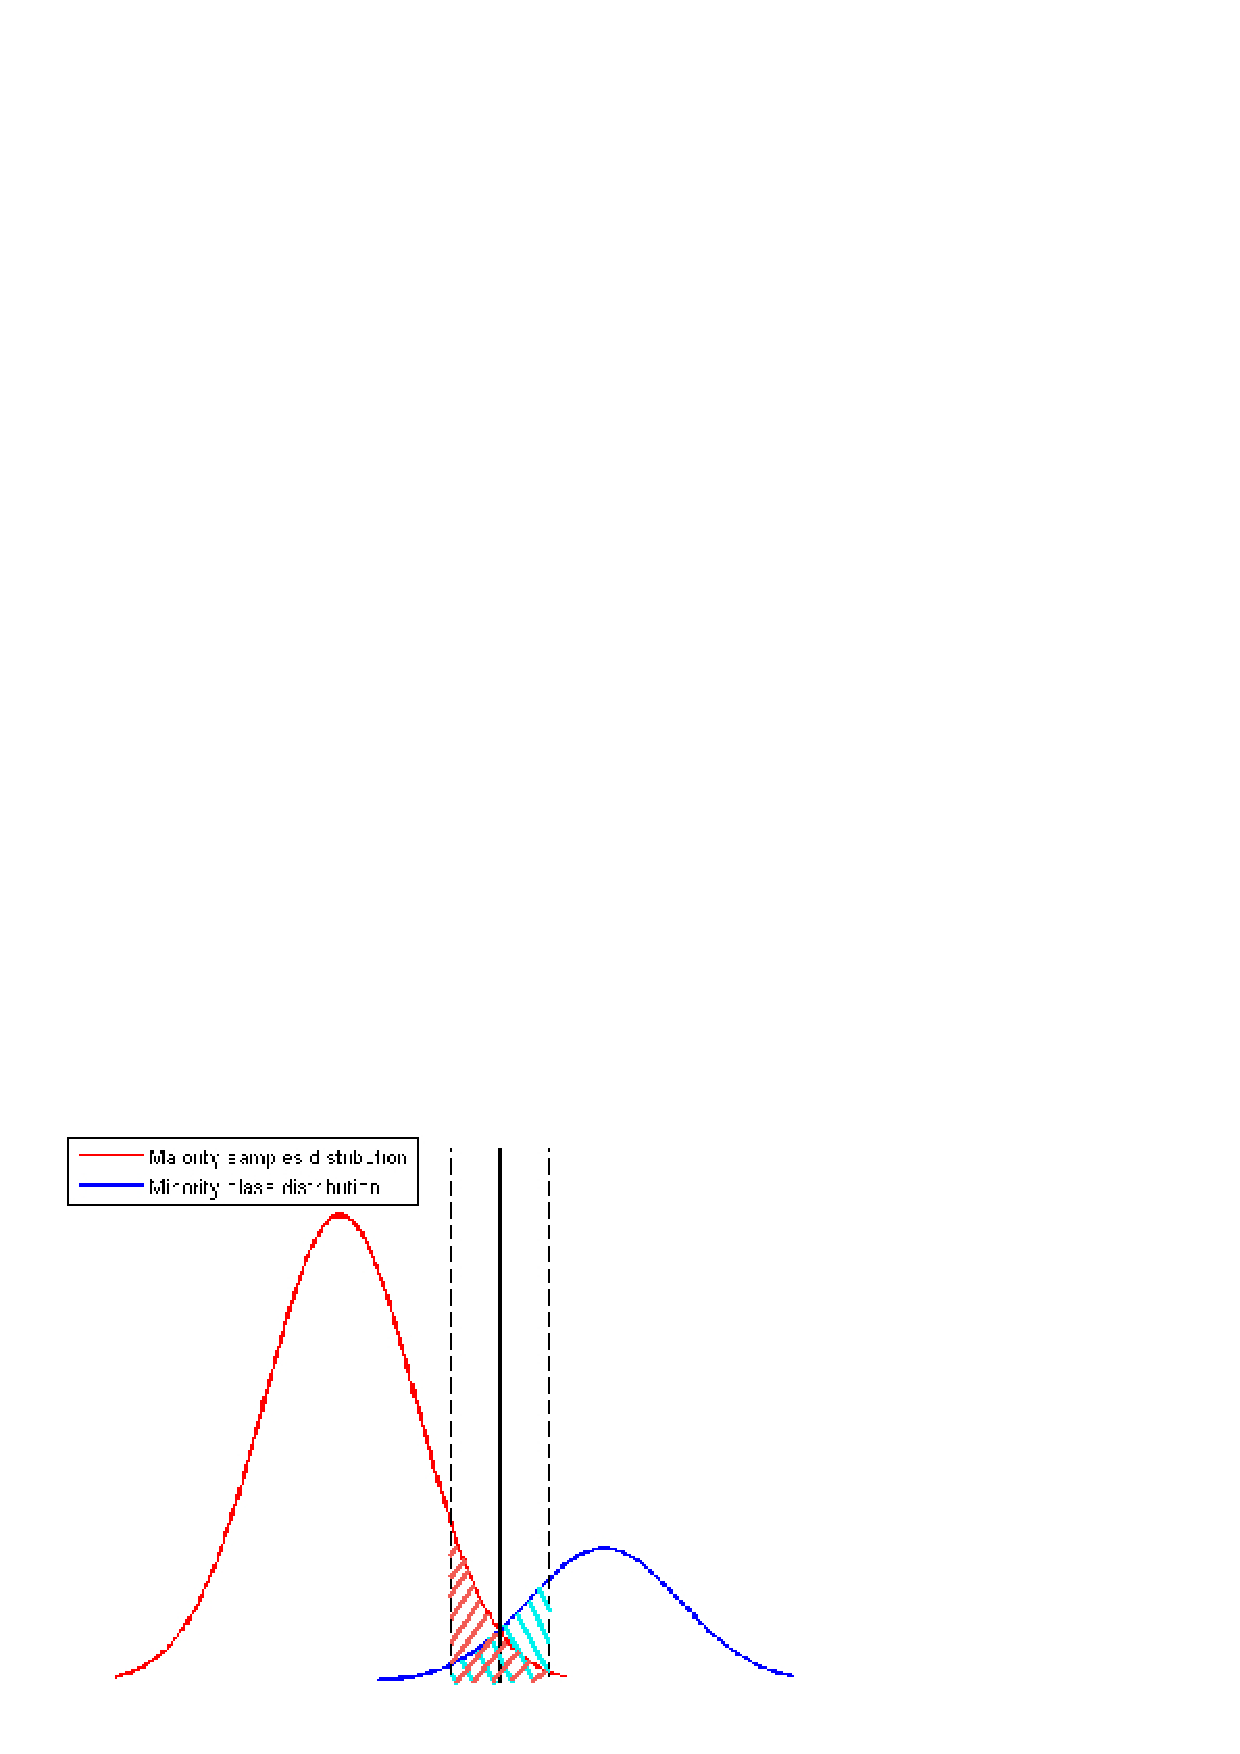
\includegraphics{Figures/lotb/al-imb-shade.pdf}}
    \caption{Data within the margin is less imbalanced than the entire data.}
    \label{fig:alimbshade}
\end{figure}

The strategy of selecting examples within the margin also strongly addresses the problems that arise from imbalanced classes.  Consider the class distributions of an imbalanced dataset presented in Figure \ref{fig:alimbshade}. The shaded region corresponds to the class distribution of the data within the margin. As shown in the figure, the imbalance ratio of the classes within the margin is much smaller than the class imbalance ratio of the entire dataset. Therefore, any selection strategy that focuses on the examples in the margin most likely ends up with a more balanced class distribution than that of the entire dataset. %Our empirical findings with various type of real-world data confirm that the imbalance ratios of the classes within the margin in real-world data are generally much lower than that of the entire data.

Throughout this section, the discussion is constrained to standard two-class classification problems using Support Vector Machines (SVMs). The next subsection presents a brief overview of SVMs, followed by the working principles of an efficient active learning algorithm in Section \ref{ALpools}. We explain the advantage of using online SVMs with the active sample selection in Section \ref{LASVM}.% In Section \ref{ES}, we then describe an early stopping heuristics for active learning.

\subsection{Support Vector Machines}
\label{SVMs}
Support Vector Machines \cite{Vapnik_1995} are well known for their strong theoretical foundations, generalization performance and ability to handle high dimensional data. In the binary classification setting, let $((x_{1}, y_{1})\cdots(x_{n}, y_{n}))$ be the training dataset where $x_i$ are the feature vectors representing the instances and  $y_i \in (-1,+1)$ be the labels of the instances.  Using the training set, SVM builds an optimum hyperplane -- a linear discriminant in a higher dimensional feature space -- that separates the two classes by the largest margin. This hyperplane is obtained by minimizing the following objective function:
\begin{equation}
\label{svm_primal}
\min_{{\bf{w}, b, \xi_{i}}}\frac{1}{2} {\bf w\cdot w}^T + C\sum_{i=1}^{N}\xi_i  \\
\end{equation}
\begin{equation}
\mbox{subject to}\left\{ \begin{array}{l} \forall i \; y_i({\bf
w}^T{\Phi(x_i)} - b)\geq 1-\xi_{i}\\ \forall i \; \xi_{i} \geq 0
\end{array} \right.
\end{equation}
where \textbf{w} is the norm of the hyperplane, $b$ is the  offset, $y_i$ are the labels, $\Phi(\cdot)$ is the mapping from input space to feature space, and $\xi_i$ are the slack variables that permit the non-separable case by allowing misclassification of training instances. In practice the convex quadratic programming (QP) problem in (\ref{svm_primal}) is solved by optimizing the dual cost function. The dual representation of (\ref{svm_primal}) is given as
\begin{equation}
\label{svm_dual}
\max W(\alpha) \equiv \sum_{i=1}^{N}\alpha_{i} - \frac{1}{2}\sum_{i,j}\alpha_i\alpha_{j}y_{i}y_{j}K({\bf x_i},{\bf x_j}) \\
\end{equation}
\begin{equation}
\mbox{subject to}\left\{ \begin{array}{l} \forall i\; 0 \leq \alpha_i \leq C\\ \sum_{i=1}^{N}\alpha_i y_i=0 \end{array} \right.
\end{equation}
where $y_i$ are the labels, $\Phi(\cdot)$ is the mapping from the input space to the feature space, $K({\bf x_i}, {\bf x_j})=\langle\Phi({\bf x_i}),\Phi({\bf x_j})\rangle$ is the kernel matrix and the $\alpha_i$'s are the \textit{Lagrange multipliers} which are non-zero only for the training instances which fall in the margin. Those training instances are called \textit{support vectors} and they define the position of the hyperplane. After solving the QP problem, the norm of the hyperplane \textbf{w} can be represented as
\begin{equation}
\label{svm_norm}
\textbf{w}=\sum_{i=1}^{n}\alpha_i\Phi(x_i)
\end{equation}

\subsection{Margin-based Active Learning with SVMs}
\label{ALpools}
Note that in (\ref{svm_norm}), only the support vectors affect the SVM solution. This means that if SVM is retrained with a new set of data which only consist of those support vectors, the learner will end up finding the same hyperplane. This emphasizes the fact that not all examples are equally important in training sets. Then the question becomes how to select the most informative examples for labeling from the set of unlabeled training examples. This section focuses on a form of selection strategy called \textit{margin-based active learning}. As was highlighted earlier, in SVMs the most informative example is believed to be the closest one to the hyperplane since it divides the \textit{version space} into two equal parts. The aim is to reduce the version space as fast as possible to reach the solution faster in order to avoid certain \textit{costs} associated with the problem. For the possibility of a non-symmetric version space, there are more complex selection methods suggested by \cite{tong02svm}, but it has been observed that the advantage of those are not significant, considering their high computational costs.

\textbf{Active Learning with Small Pools:}
 The basic working principle of margin-based active learning with SVMs is: $i)$ train an SVM on the existing training data, $ii)$ select the closest example to the hyperplane, and $iii)$ add the new selected example to the training set and train again. In classical active learning \cite{tong02svm}, the search for the most informative example is performed over the entire dataset. Note that, each iteration of active learning involves the recomputation of each training example's distance to the new hyperplane. Therefore, for large datasets, searching the entire training set is a very time consuming and computationally expensive task.

One possible remedy for this performance bottleneck is to use the ``59 trick'' \cite{Smola_2000}, which alleviates a full search through the entire dataset, approximating the most informative examples by examining a small constant number of randomly chosen samples. The method picks $L$ ($L \ll$ \# training examples) random training samples in each iteration and selects the best (closest to the hyperplane) among them. Suppose, instead of picking the closest example among all the training samples $X_N=(x_1, x_2, \cdots ,x_N)$ at each iteration, we first pick a random subset $X_L$, $L\ll N$ and select the closest sample $x_i$ from $X_L$ based on the condition that $x_i$ is among the top $p\%$ closest instances in $X_N$ with probability $(1-\eta)$. Any numerical modification to these constraints can be met by varying the size of $L$, and is independent of $N$. To demonstrate, the probability that at least one of the $L$ instances is among the closest $p$ is $1-(1-p)^L$. Due to the requirement of $(1-\eta)$ probability, we have
\begin{equation}
1-(1-p)^L = 1-\eta
\end{equation}
which follows the solution of $L$ in terms of $\eta$ and $p$
\begin{equation}
L={{\log \eta} \;/\;{\log(1-p)}}
\end{equation}
For example, the active learner will pick one example, with $95\%$ probability, that is among the top $5\%$ closest instances to the hyperplane, by randomly sampling only $\lceil \log(.05)/\log(.95) \rceil = 59$ examples regardless of the training set size. This approach scales well since the size of the subset $L$ is independent of  the training set size $N$, requires significantly less training time and does not have an adverse effect on the classification performance of the learner.

%\begin{figure*}[t]
%    \centering
%        \scalebox{0.34}{\includegraphics{Figures/lotb/rpal.pdf}}
%    \caption{Comparison of PRBEP and g-means of RS, AL(full search) and AL(random pool). The training times of AL(full search) vs. AL(random pool) until saturation in seconds are: 272 vs. 50 (grain), 142 vs. 32 (ship) and 126 vs. 13 (USPS). AL(random pool) is 4 to 10 times faster than AL(full search) with similar prediction performance.}
%    \label{fig:rpal}
%\end{figure*}

%Figure \ref{fig:rpal} shows the comparisons of PRBEP and g-means performances of AL(random pool) and the traditional active learning method AL(full search) \cite{Tong_2002}. For the random pool strategy, we set $L=59$ which means we pick 59 random examples to form the query pool  at each learning step and pick the closest example to the hyperplane from this pool. RS corresponds to the random sampling strategy where the examples are selected randomly. As Figure \ref{fig:rpal} depicts, active learning method with small pools achieves as good prediction performance as the traditional active learning method. Moreover, the random pool strategy is 4 to 10 times faster than traditional active learning for the given datasets.

\subsection{Active Learning with Online Learning}
\label{LASVM}
Online learning algorithms are usually associated with problems where the complete training set is not available. However, in cases where the complete training set \textit{is} available, the computational properties of these algorithms can be leveraged for faster classification and incremental learning. Online learning techniques can process new data presented one at a time,  either as the result of active learning or random selection, and can integrate the information of the new  data to the system without training on all previously seen data, thereby allowing models to be constructed incrementally. This working principle of online learning algorithms leads to speed improvements and a reduced memory footprint, making the algorithm applicable to very large datasets. More importantly, this incremental learning principle suits the nature of active learning in a much more naturally than the batch algorithms. Empirical evidence indicates that a single presentation of each training example to the algorithm is sufficient to achieve training errors comparable to those achieved by the best minimization of the SVM objective~\cite{Bordes_2005}.% In section \ref{ES} we also show that if we use an early stopping criteria in active sample selection, we do not have to introduce all training examples to the learner.
%\subsection{Active Learning with Early Stopping}
%\label{ES}
%Early stopping criteria is advantageous to active learning since it converges to the solution faster than the random sample selection method. A theoretically sound method to stop training is when the examples in the margin are exhausted. To check if there are still unseen training examples in the margin, the distance of the new selected example is compared against the support vectors of the current model. If the new selected example by active learning (closest to the hyperplane) is not closer than any of the support vectors, we conclude that the margin is exhausted. A practical implementation of this idea is to count the number of support vectors during the active learning training process. If the number of the support vectors stabilizes, it implies that all possible support vectors have been selected by the active learning method.

%\begin{figure}[b]
%    \hspace{-10mm}
%        \scalebox{0.3}{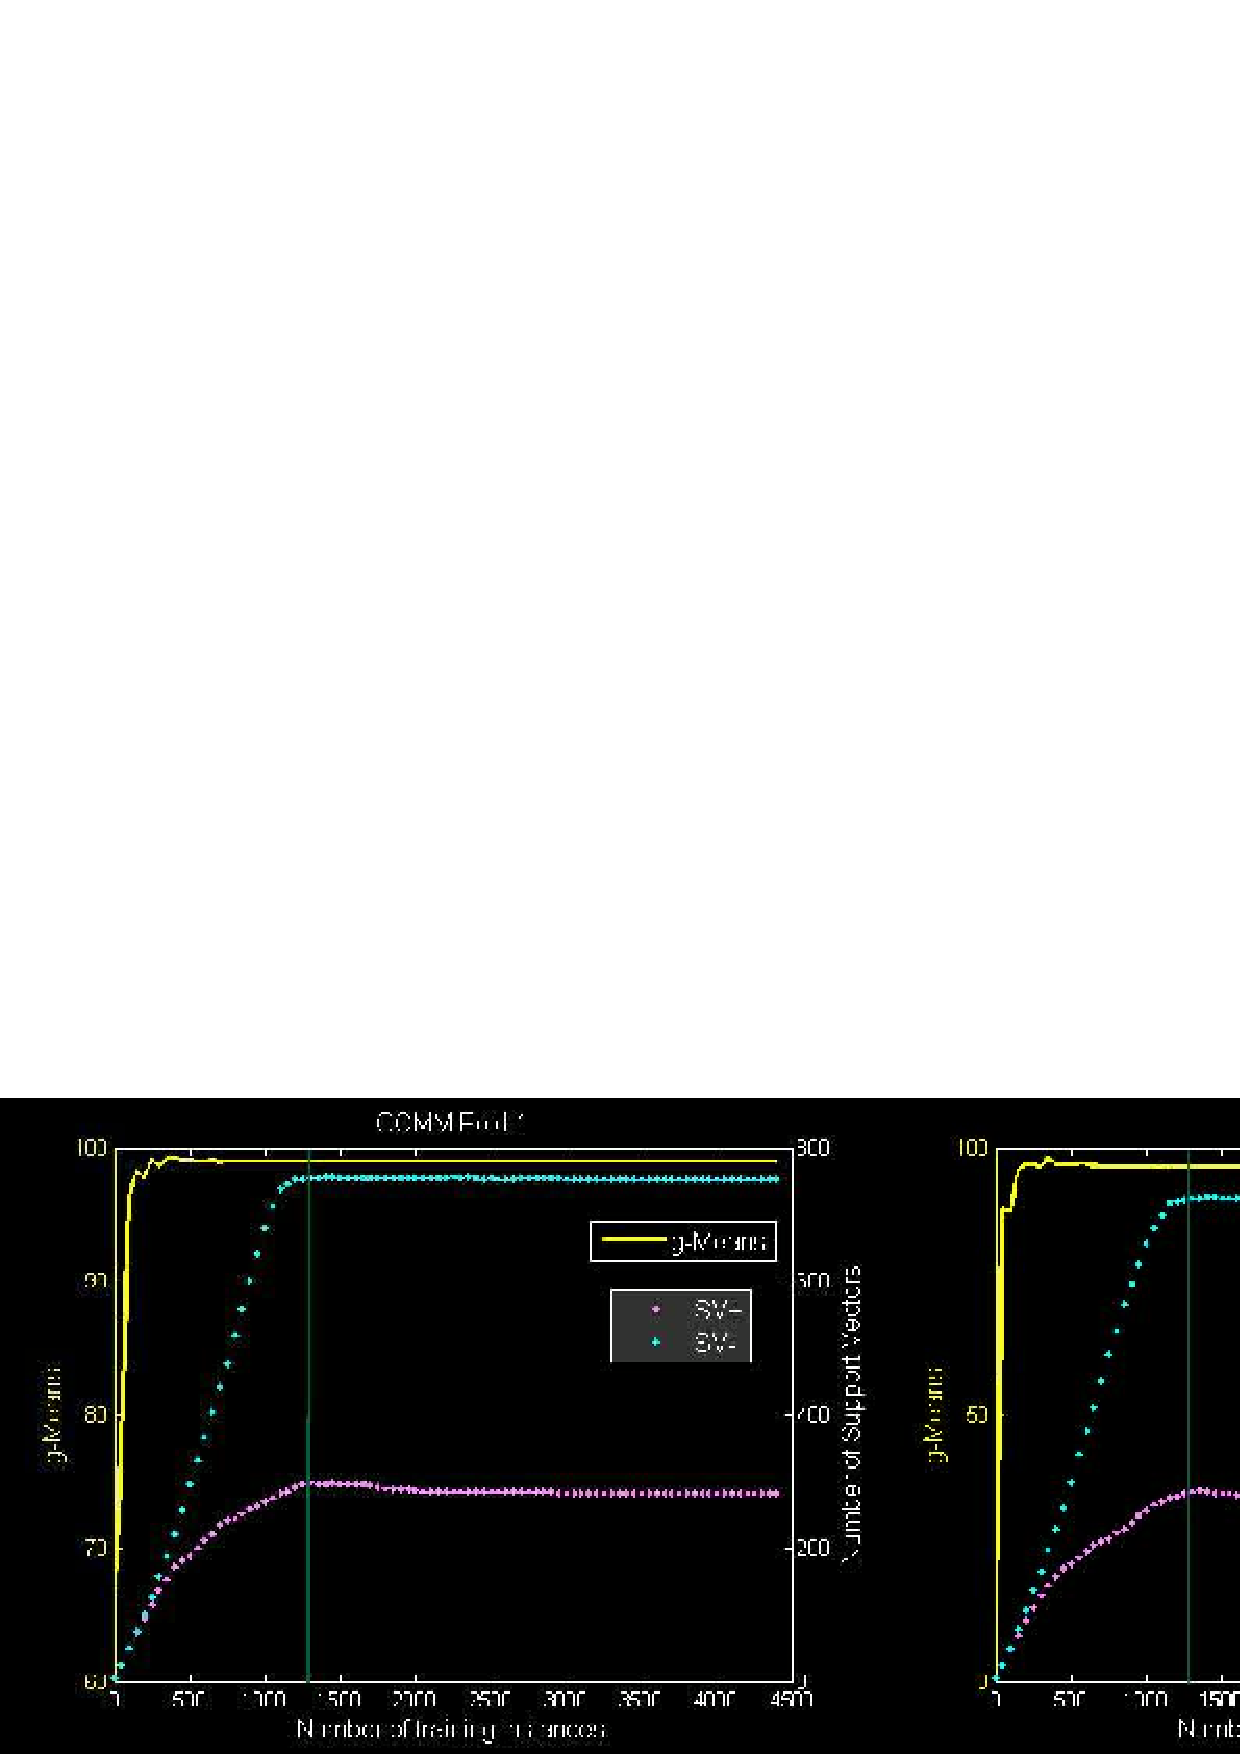
\includegraphics{Figures/lotb/comm.pdf}}
%    \caption{3-fold cross-validation results for the training set of the category COMM in CiteSeer dataset. Vertical lines correspond to early stopping points.}
%    \label{fig:comm}
%\end{figure}

%In order to analyze this method, we conducted a 3-fold cross-validation on one of the datasets (see Figure \ref{fig:comm}). In cross-validation, $2/3$ of the training set is used for training and the remaining $1/3$ is reserved as the hold-out dataset. Since the training set distribution is representative of the test set distribution, we believe that the algorithm's behavior would most likely be the same in the test set. As can be seen in Figure \ref{fig:comm}, in active learning setups, after using certain number of labeled training data, the number of support vectors saturates and  g-means levels off as well. Those graphs support the idea that the model does not change after the system observes enough informative samples. Further, adding more training data after this point does not make a remarkable change in the model and consequently in prediction performance. Notice that in Figure \ref{fig:comm} the vertical line indicates the suggested early stopping point and it is approximately equal in all three folds. As a result, we adopt the early stopping strategy of examining the number of support vectors in the entire training datasets without performing cross-validation.

\subsection{Performance Metrics}
Classification accuracy is not a good metric to evaluate classifiers in applications facing class imbalance problems.  SVMs have to achieve a tradeoff between maximizing the margin and minimizing the empirical error. In the non-separable case, if the misclassification penalty $C$ is very small, the SVM learner simply tends to classify every example as negative. This extreme approach maximizes the \textit{margin} while making no classification errors on the negative instances. The only error is the cumulative error of the positive instances which are already few in numbers. Considering an imbalance ratio of $99$ to $1$, a classifier that classifies everything as negative, will be $99\%$ accurate. Obviously,  such a scheme would not have any practical use as it would be unable to identify  positive instances.

For the evaluation of these results, it is useful to consider  several other prediction performance metrics such as g-means, AUC and PRBEP which are commonly used in imbalanced data classification. g-means \cite{Kubat_1997} is denoted as $g=\sqrt{sensitivity \cdot specificity}$ where sensitivity is the accuracy on the positive instances given as $True Pos./(True Pos.+False Neg.)$ and specificity is the accuracy on the negative instances given as $True Neg./(True Neg.+False Pos.)$.

The Receiver Operating Curve (ROC) displays the relationship between sensitivity and specificity at all possible thresholds for a binary classification scoring model, when applied to independent test data. In other words, ROC curve is a plot of the true positive rate against the false positive rate as the decision threshold is changed. The \textit{area under the ROC curve} (AUC) is a numerical measure of a model's discrimination performance and shows how successfully and correctly the model ranks and thereby separates the positive and negative observations. Since the AUC metric evaluates the classifier across the entire range of decision thresholds, it gives a good overview about the performance when the operating condition for the classifier is unknown or the classifier is expected to be used in situations with significantly different class distributions.

Precision Recall Break-Even Point (PRBEP) is another commonly used performance metric for imbalanced data classification. PRBEP is the accuracy of the positive class at the threshold where precision equals to recall. Precision is defined as $True Pos./(True Pos.+False Pos.)$ and recall is defined as $True Pos./(True Pos.+False Neg.)$


%\begin{table}[t!]
%\caption{Overview of the datasets.} \centering \small
%\begin{tabular}{l|l|r@{\hspace{2mm}}r@{\hspace{2mm}}r@{\hspace{2mm}}r|c c}
%\hline
%\multicolumn{2}{c|}{Dataset}&\#Feat.&\#Pos&\#Neg&Ratio&c&$\gamma$\\
%\hline\hline
%\multirow{5}{5mm}{\begin{sideways}\parbox{13mm}{Reuters}\end{sideways}}&Crude&8315&389&7381&19.0&2&1\\
%&Grain&8315&433&7337&16.9&2&1\\
%&Interest& 8315 &347&7423&21.4&1&2\\
%&Money-fx& 8315 &538&7232&13.4&1&0.5\\
%&Ship& 8315 &197&7573&38.4&1&0.5\\
%&Wheat& 8315 &212&7558&35.7&1&0.5\\
%\hline
%\multirow{5}{5mm}{\begin{sideways}\parbox{12mm}{CiteSeer}\end{sideways}}
%&AI& 6946 &1420&5353&4.3&50&0.1\\
%&COMM& 6946 &1252&5341&4.2&50&0.1\\
%&Crypt& 6946 &552&6041&11.0&50&0.1\\
%&DB& 6946 &819&5775&7.1&50&0.1\\
%&OS& 6946 &262&6331&24.2&50&0.1\\
%\hline
%\multirow{2}{5mm}{\begin{sideways}\parbox{8mm}{UCI}\end{sideways}}
%&Abalone-7& 9 &352&3407&9.7&100&0.01\\
%&Letter-A&16 &710&17290&24.4&10&0.01\\
%&Satimage&36&415&4020&9.69&50&0.001\\
%\hline
%\multicolumn{2}{c|}{USPS}& 256 &1232&6097&5.0&1000&2\\
%\hline
%\multicolumn{2}{c|}{MNIST-8}& 780 &5851&54149&9.3&1000&0.02\\
%\hline
%\end{tabular}
%\label{tbl:overview}
%\end{table}

%\subsection{Datasets}
%We study the performance of the algorithm on various benchmark real-world datasets. The overview of the datasets are given in Table \ref{tbl:overview}. The \emph{Reuters-21578} is a popular text mining benchmark dataset. We test the algorithms with 8 of the top 10 most populated categories of \emph{Reuters-21578}. We did not use categories `earn' and `acq' since their class imbalance ratios are not high enough. As a text dataset, we also used 5 categories from CiteSeer\footnote{http://citeseer.ist.psu.edu} data. We used 4 benchmark datasets from the popular UCI Machine Learning Repository as well. \emph{Letter} and \emph{satimage} are image datasets. The `letter A' is used as the positive class in \emph{letter} and `class 4' (damp grey soil) is used as positive class in \emph{satimage}. \emph{Abalone} is a biology dataset where the instances labeled as `class 7' are used to form the positive class. \emph{MNIST} and \emph{USPS} are OCR data of handwritten digits and `digit 8' is used as a positive class in \emph{Mnist}. \emph{Adult} is a census dataset to predict if the income of a person is greater than 50K based on several census parameters, such as age, education, marital status etc. The training set consists of 32,562 instances and the class imbalance ratio is 3. \emph{Waveform} is a popular artificial dataset used commonly in simulation studies. These datasets cover a wide range of data imbalance ratios.

\subsection{Experiments and Empirical Evaluation}
\label{lotb_experiments}
%We first conduct experiments to compare the performance of AL(random pool) strategy with the traditional active learning method, AL(full search). The results show that with the proposed method, we can make faster active learning without sacrificing any prediction performance. In the rest of the section, we refer to AL(random pool) as AL since it is the only active learning method that we used afterwards.

%\begin{figure}[b!]
%        \scalebox{0.47}{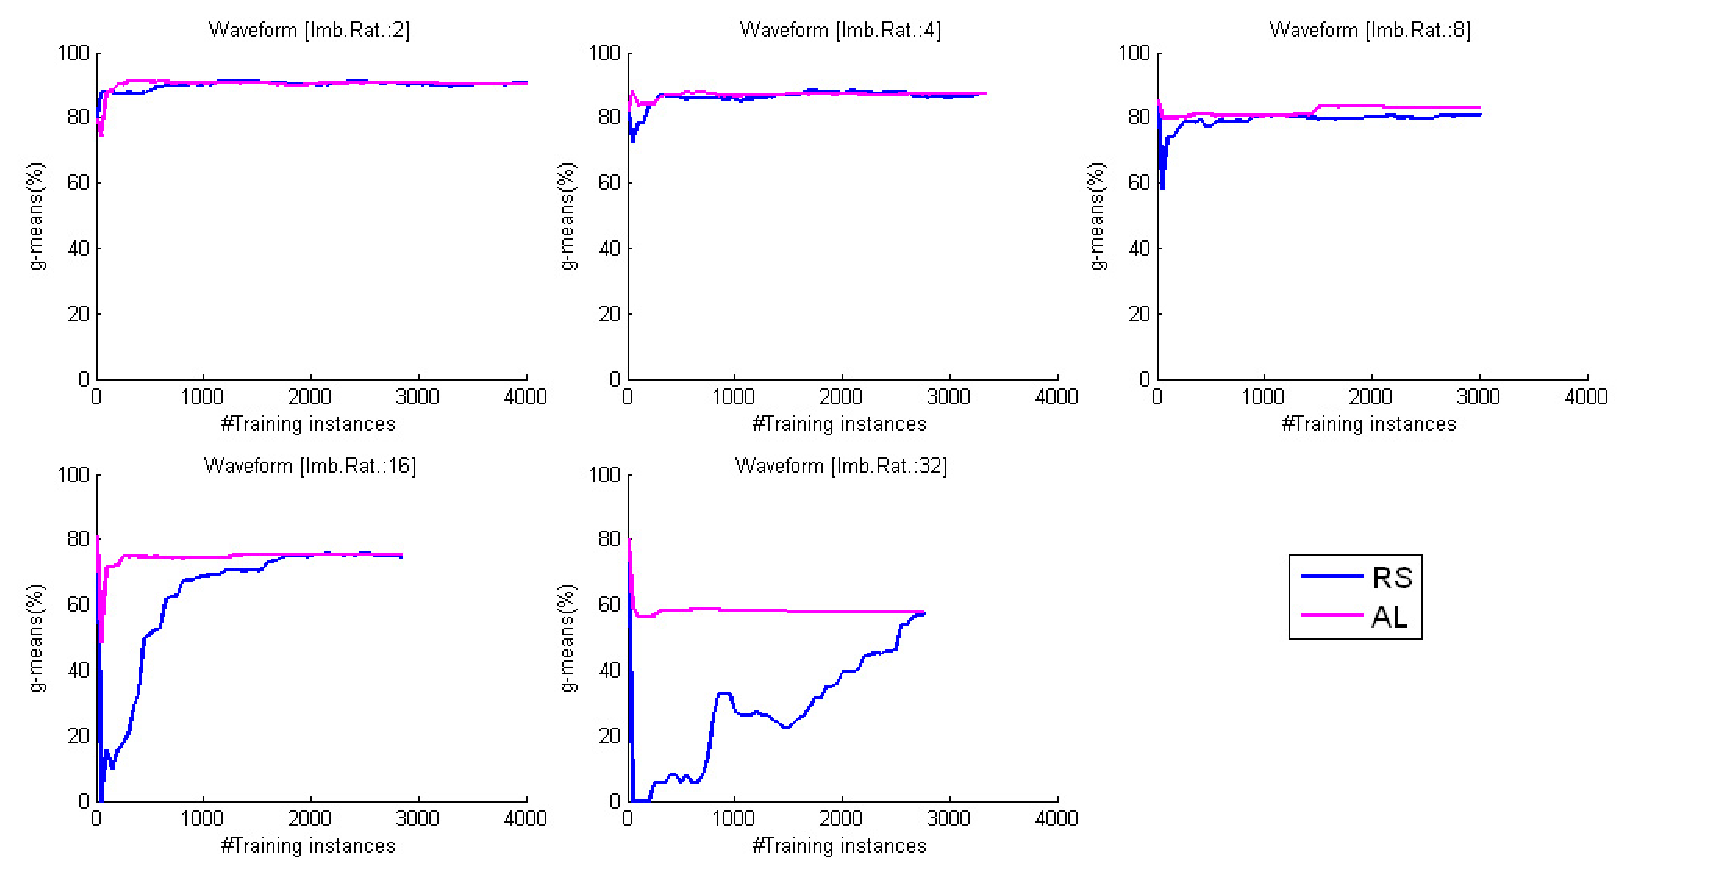
\includegraphics{Figures/lotb/wfall.eps}}
%    \caption{Comparison of g-means of AL and RS on the waveform datasets with different imbalance ratios (Imb.R.=2, 4, 8, 16, 32).}
%    \label{fig:wfall}
%\end{figure}
\begin{figure}[b!]
\begin{center}
\vspace{-4mm}
\subfigure {
\includegraphics[width=55mm]{Figures/lotb/adultall_1.jpg}
}
\subfigure {
\includegraphics[width=55mm]{Figures/lotb/adultall_2.jpg}
}\\
\vspace{-2mm}
\subfigure {
\includegraphics[width=55mm]{Figures/lotb/adultall_3.jpg}
}
\subfigure {
\includegraphics[width=55mm]{Figures/lotb/adultall_4.jpg}
}
 \caption{Comparison of PRBEP of AL and RS on the adult datasets with different imbalance ratios (Imb.R.=3, 10, 20, 30).}
    \label{fig:adultall}
\end{center}
\end{figure}


%In order to make a thorough analysis on the effect of AL(random pool) to imbalanced data classification, we examine its performance by varying class imbalance ratios using two performance metrics.
We study the performance of the algorithm on various benchmark real-world datasets, including MNIST, USPS, several categories of Reuters-21578 collection, five topics from CiteSeer, and three datasets from the UCI repository. The characteristics of the datasets are outlined in \cite{Ertekin2_2007}. In the experiments, an early stopping heuristic for active learning is employed, since it has been shown that active learning converges to the solution faster than the random sample selection method \cite{Ertekin2_2007}. A theoretically sound method to stop training is when the examples in the margin are exhausted. To check if there are still unseen training examples in the margin, the distance of the newly selected example is compared against the support vectors of the current model. If the new selected example by active learning (closest to the hyperplane) is not closer than any of the support vectors, it is concluded that the margin is exhausted. A practical implementation of this idea is to count the number of support vectors during the active learning training process. If the number of the support vectors stabilizes, it implies that all possible support vectors have been selected by the active learning method.

\begin{table*}[t!]\centering{
\caption{Comparison of g-means and AUC for AL and RS with entire training data (Batch).
SV ratios are given at the saturation point. Data efficiency corresponds to the percentage of training instances which AL processes to reach saturation.}
\begin{tabular}{l|l|r r|r r||r|r|c}
\hline
\multicolumn{2}{c|}{\multirow{2}{1cm}{Dataset}}
&\multicolumn{2}{c|}{g-means (\%)}
&\multicolumn{2}{c||}{AUC (\%)}
&Imb.&SV- /&\multirow{2}{12mm}{Data Efficiency}
\\
\cline{3-6}
\multicolumn{2}{c|}{}&Batch&AL&Batch&AL&Rat.&SV+\\
\hline\hline
\multirow{8}{1mm}{\begin{sideways}\parbox{12mm}{Reuters}\end{sideways}}
&Corn&85.55&86.59&99.95&99.95&41.9&3.13&11.6\%\\
&Crude&88.34&89.51&99.74&99.74&19.0&2.64&22.6\%\\
&Grain&91.56&91.56&99.91&99.91&16.9&3.08&29.6\%\\
&Interest&78.45&78.46&99.01&99.04&21.4&2.19&30.9\%\\
&Money-fx&81.43&82.79&98.69&98.71&13.4&2.19&18.7\%\\
&Ship&75.66&74.92&99.79&99.80&38.4&4.28&20.6\%\\
&Trade&82.52&82.52&99.23&99.26&20.1&2.22&15.4\%\\
&Wheat&89.54&89.55&99.64&99.69&35.7&3.38&11.6\%\\
\hline
\multirow{5}{1mm}{\begin{sideways}\parbox{12mm}{CiteSeer}\end{sideways}}
&AI&87.83&88.58&94.82&94.69&4.3&1.85&33.4\%\\
&COMM&93.02&93.65&98.13&98.18&4.2&2.47&21.3\%\\
&CRYPT&98.75&98.87&99.95&99.95&11.0&2.58&15.2\%\\
&DB&92.39&92.39&98.28&98.46&7.1&2.50&18.2\%\\
&OS&91.95&92.03&98.27&98.20&24.2&3.52&36.1\%\\
\hline
\multirow{3}{1mm}{\begin{sideways}\parbox{6mm}{UCI}\end{sideways}}
&Abalone-7&100.0&100.0&100.0&100.0&9.7&1.38&24.0\%\\
&Letter-A&99.28&99.54&99.99&99.99&24.4&1.46&27.8\%\\
&Satimage&82.41&83.30&95.13&95.75&9.7&2.62&41.7\%\\
\hline
\multicolumn{2}{c|}{USPS}&99.22&99.25&99.98&99.98&4.9&1.50&6.8\%\\
\hline
\multicolumn{2}{c|}{MNIST-8}&98.47&98.37&99.97&99.97&9.3&1.59&11.7\%\\
\hline
\end{tabular}
\label{tbl:AUC}

}
\end{table*}

As the first experiment, examples are randomly removed from the minority class in \emph{Adult} dataset to achieve different data imbalance ratios, comparing SVM-based active learning (AL) and random sampling (RS).\footnote{Here, the random process is assumed to be uniform; examples are selected with equal probability from the available pool.} \josh {I don't understand the following sentence} \seyda{Addressed.}  For brevity, AL with small pools is referred to as AL since the small pools heuristic is utilized for all active learning methods considered later. Comparisons of PRBEP in Figure \ref{fig:adultall} show an interesting behavior. As the class imbalance ratio is increased, AL curves display peaks in the early steps of the learning. This implies that by using an early stopping criteria AL can give higher prediction performance than RS can possibly achieve even after using all the training data. The learning curves presented in Figure \ref{fig:adultall} demonstrate that the addition of instances to a model's training after finding those most informative instances can be detrimental to the prediction performance of the classifier, since this may cause the model to suffer from overfitting. Figure \ref{fig:adultall} curves show that generalization can peak to a level above that can be achieved by using all available training data. In other words,it is possible to achieve better classification performance from a small informative subset of the training data than what can achieved using all available training data. This finding agrees with \cite{Schohn_2000} and strengthens the idea of applying an early stopping to active learning algorithms. \josh{say a few sentences why this may be the case? one can easily be surprised to learn that throwing away data can be a good thing.}\seyda{Added a few more sentences above and also a reference.}

For further comparison of the performance of the performance of a model built on all available data (Batch) and AL subject to early halting criteria, refer to Table~\ref{tbl:AUC}, comparing  the g-means and the AUC values for these two methods. The data efficiency column for AL indicates that by processing only a portion of the examples from the training set, AL can achieve similar or even higher generalization performance than that of Batch which sees all the training examples. Another important observation from Table \ref{tbl:AUC} is that support vector imbalance ratios in the final models are much less than the class imbalance ratios of the datasets. This confirms the discussion of Figure \ref{fig:alimbshade}. The class imbalance ratio within the margins are much less than the class imbalance ratio of the entire data and active learning can be used to reach those informative examples which most likely become support vectors without seeing all the training examples.


\begin{figure}[t!]
    \centering
        \scalebox{0.4}{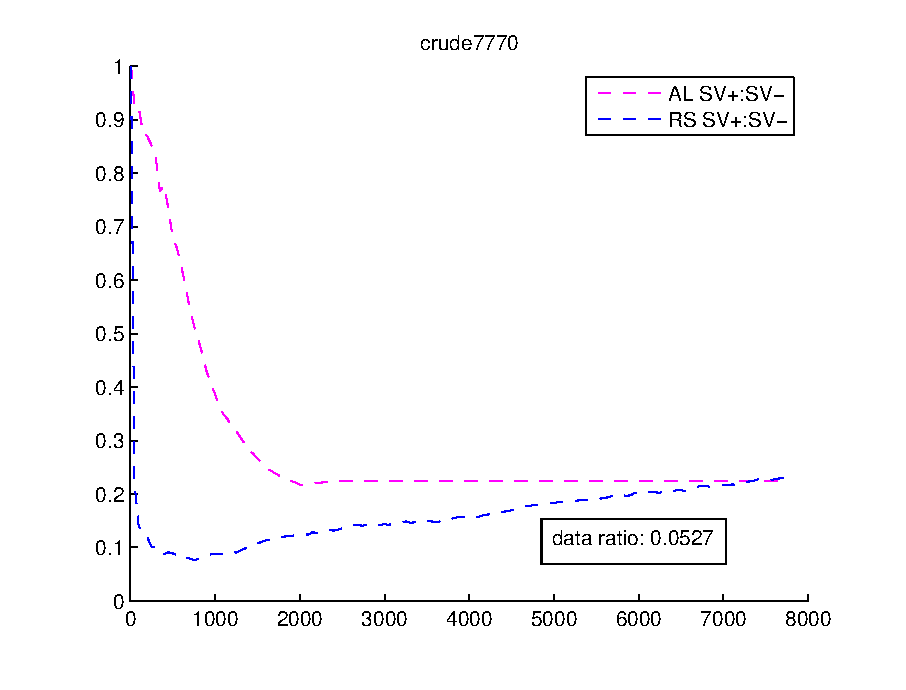
\includegraphics{Figures/lotb/cruderatio.eps}}
    \caption{Support Vector ratios in AL and RS}
    \label{cruderatio}
\end{figure}

Figure \ref{cruderatio} investigates how the number of support vectors changes when presented with examples selected according to  AL and RS. Because the base rate of the dataset gathered by RS approaches that of the example pool, the support vector imbalance ratio quickly approaches the data imbalance ratio. As learning continues, the learner should gradually see all the instances within the final margin and the support vector imbalance ratio decreases. At the end of training with RS, the support vector imbalance ratio is the data imbalance ratio within the margin. The support vector imbalance ratio curve of AL is drastically different than RS. AL intelligently picks the instances closest to the margin in each step. Since the data imbalance ratio within the margin is lower than data imbalance ratio, the support vectors in AL are more balanced than RS during learning. Using AL, the model saturates by seeing only 2000 (among 7770) training instances and reaches the final support vector imbalance ratio. Note that both methods achieve similar support vector imbalance ratios when learning finishes, but AL achieves this in the early steps of the learning.

It is also interesting to consider the performance of active learning as a selection heuristic in light of more conventional sampling strategies. Here, AL is compared to traditional under-sampling of the majority class (US), and an oversampling method (SMOTE), both examples of resampling techniques which require preprocessing. It has been shown that oversampling at random does not help to improve prediction performance \cite{Japkowicz_2002} therefore a more complex oversampling method is required.  Synthetic Minority Oversampling Technique (SMOTE) oversamples the minority class by creating synthetic examples rather than with replacement. The $k$ nearest positive neighbors of all positive instances are identified and synthetic positive examples are created and placed randomly along the line segments joining the $k$ minority class nearest neighbors.


For additional comparison, the method of assigning different costs (DC) to the positive and negative classes as the misclassification penalty parameter is examined. For instance, if the imbalance ratio of the data is 19:1 in favor of the negative class, the cost of misclassifying a positive instance is set to be 19 times greater than that of misclassifying a negative one. We use the online SVM package LASVM\footnote{Available at \texttt{http://leon.bottou.org/projects/lasvm}} in all experiments. Other than the results of the methods addressing the class imbalance problem, the results of Batch algorithm with the original training set are provided to form a baseline. LASVM is run in random sampling mode for US, SMOTE and DC.

\begin{figure*}[t!]
    \hspace{-5mm}
        \scalebox{0.48}{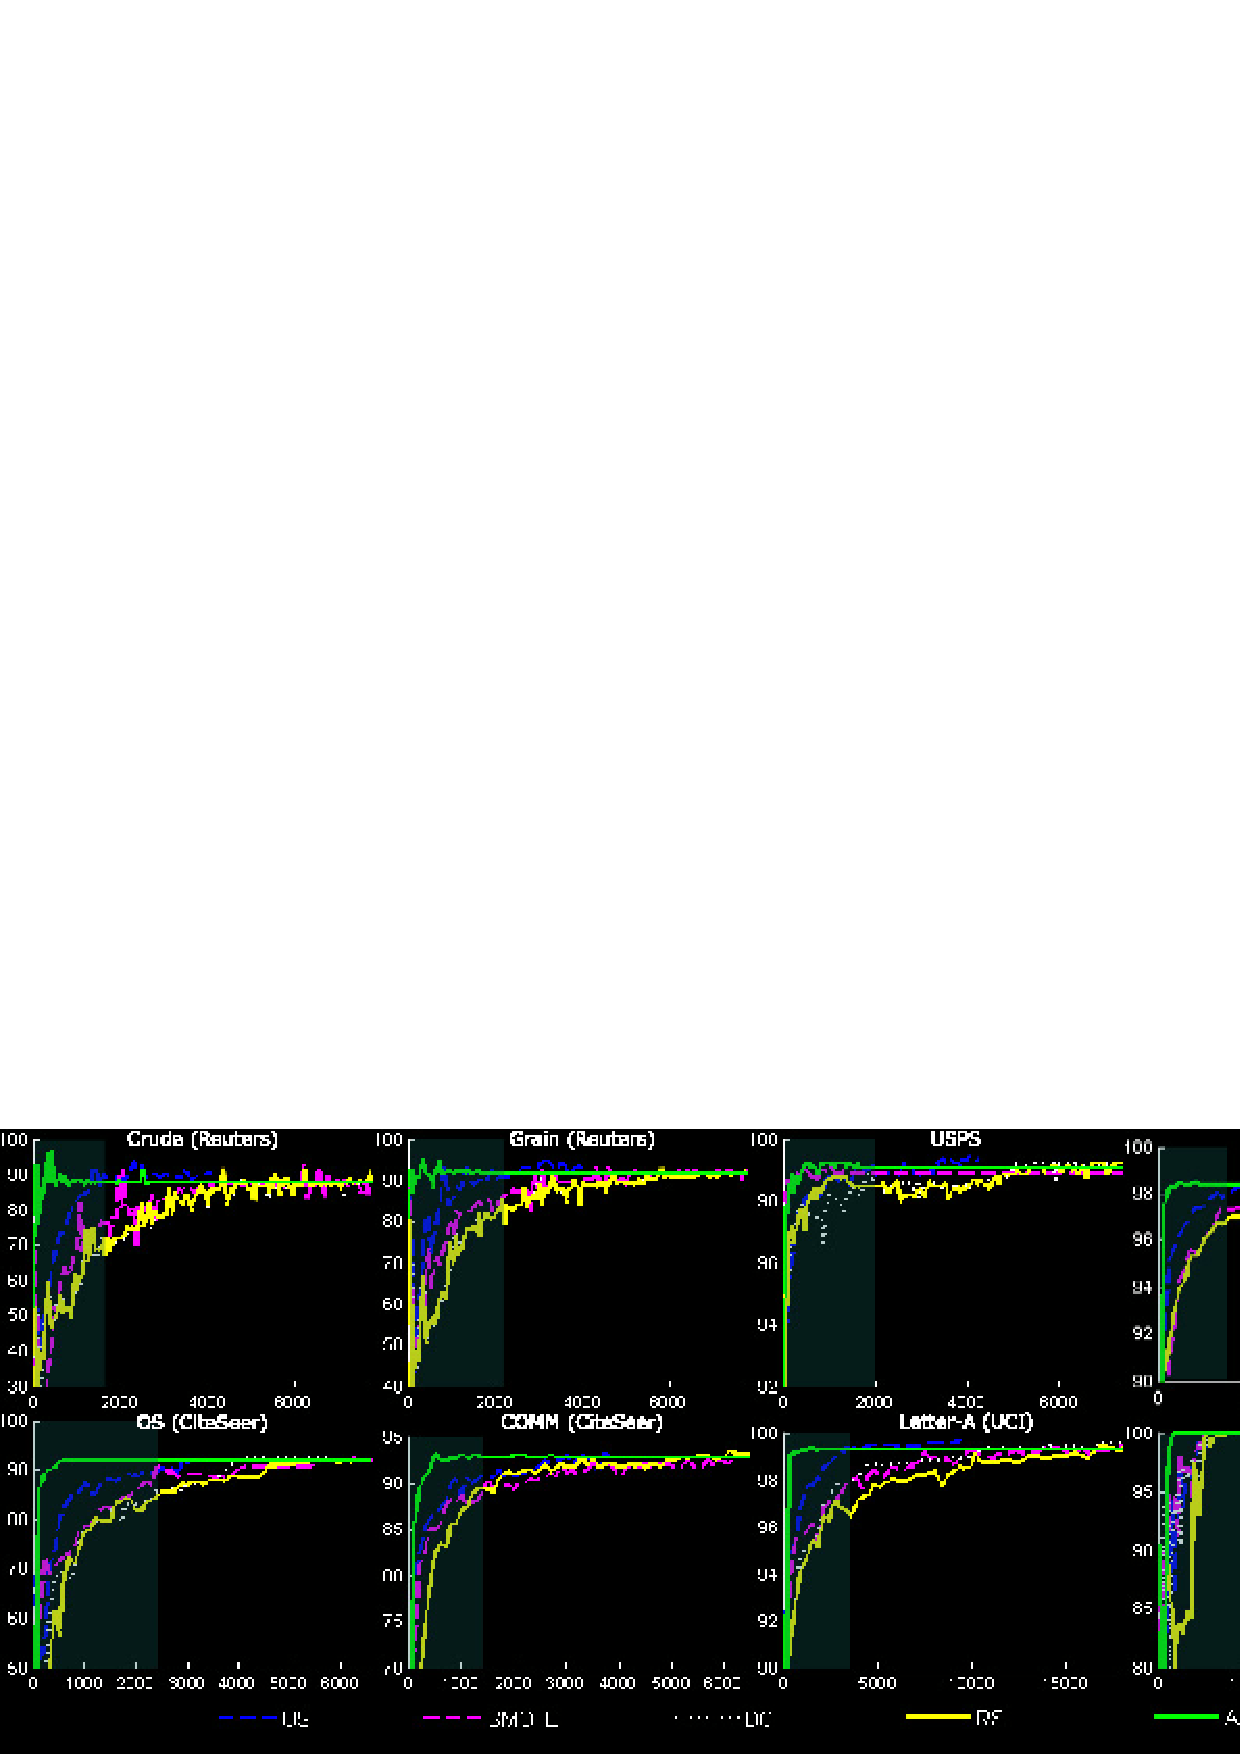
\includegraphics{Figures/lotb/big8.pdf}}
    \caption{Comparisons of g-means. The right border of the shaded area corresponds to the early stopping point.}
    \label{eightgraphs}
\end{figure*}


We present the comparisons of the methods for g-means performance metric for several datasets in Figure \ref{eightgraphs}. The right border of the shaded pink area is the place where the aforementioned early stopping strategy is applied.  The curves in the graphs are averages of 10 runs. For completeness, all  AL experiments were allowed to continue to select examples until exhaustion, bypassing any early stopping.  Table \ref{tbl:results} presents the PRBEP of the methods and the total running times of the SMOTE and AL on 18 benchmark and real-world datasets. The results for active learning in Table \ref{tbl:results} depict the results in the early stopping points. The results for the other methods in Table \ref{tbl:results} depict the values at the end of the curves--- when trained with the entire dataset--- since those methods do not employ any early stopping criteria. We did not apply early stopping criteria to the other methods because, as observed from Figure \ref{eightgraphs}, no early stopping criteria would achieve a comparable training time with of AL's training time without a significant loss in their prediction performance based on convergence time. The other methods converge to similar levels of g-means when nearly all training instances are used, and applying an early stopping criteria would have little, if any, effect on their training times.

\begin{table*}[b!]\centering{
\caption{Comparison of PRBEP and training time. }\small
\begin{tabular}{l|l|r r r r r|r r}
\hline
\multicolumn{2}{c|}{Metric}&\multicolumn{5}{c|}{PRBEP}&\multicolumn{2}{c}{Training time (sec.)}\\
\hline
\multicolumn{2}{c|}{Dataset}&Batch&US&SMOTE&DC&AL&SMOTE&AL\\
\hline
\hline
\multirow{8}{5mm}{\begin{sideways}\parbox{13mm}{Reuters}\end{sideways}}
&Corn&91.07&78.57&91.07&89.28&89.29&87&16\\
&Crude&87.83&85.70&87.83&87.83&87.83&129&41\\
&Grain&92.62&89.93&91.44&91.94&91.94&205&50\\
&Interest&76.33&74.04&77.86&75.57&75.57&116&42\\
&Money-fx&73.74&74.30&75.42&75.42&76.54&331&35\\
&Ship&86.52&86.50&88.76&89.89&89.89&49&32\\
&Trade&77.77&76.92&77.77&77.78&78.63&215&38\\
&Wheat&84.51&81.61&84.51&84.51&85.92&54&25\\
\hline
\multirow{5}{5mm}{\begin{sideways}\parbox{12mm}{CiteSeer}\end{sideways}}
&AI&78.80&80.68&78.99&78.79&79.17&1402&125\\
&COMM&86.59&86.76&86.59&86.59&86.77&1707&75\\
&CRYPT&97.89&97.47&97.89&97.89&97.89&310&19\\
&DB&86.36&86.61&86.98&86.36&86.36&526&41\\
&OS&84.07&83.19&84.07&84.07&84.07&93&23\\
\hline
\multirow{3}{5mm}{\begin{sideways}\parbox{6mm}{UCI}\end{sideways}}
&Abalone-7&100.0&100.0&100.0&100.0&100.0&16&4\\
&Letter-A&99.48&96.45&99.24&99.35&99.35&86&3\\
&Satimage&73.46&68.72&73.46&73.93&73.93&63&21\\
\hline
\multicolumn{2}{c|}{USPS}&98.44&98.44&98.13&98.44&98.75&4328&13\\
\hline
\multicolumn{2}{c|}{MNIST-8}&97.63&97.02&97.74&97.63&97.74&83,339&1,048\\
\hline

\end{tabular}
\label{tbl:results}
}
\end{table*}

Since AL involves discarding some instances from the training set, it can be perceived as a type of under-sampling method. Unlike traditional US, which discards majority samples randomly, AL performs an intelligent search for the most informative ones adaptively in each iteration according to the current hyperplane. Datasets where class imbalance ratio is high such as \emph{corn}, \emph{wheat}, \emph{letter} and \emph{satimage} observe significant decrease in PRBEP of US (see Table 3). Note that US's under-sampling rate for the majority class in each category is set to the same value as the final support vector ratio which AL reaches in the early stopping point and RS reaches when it sees the entire training data. Although the class imbalance ratio provided to the learner in AL and US are the same, AL achieves significantly better PRBEP performance metric than US. The Wilcoxon signed-rank test (2-tailed) reveals that the zero median hypothesis can be rejected at the significance level 1\% (p=0.0015), implying that AL performs statistically better than US in these 18 datasets. These results reveal the importance of using the informative instances for learning.

%Table \ref{tbl:rankresults} presents the rank of PRBEP prediction performance of the five approaches in a variety of datasets. The values in bold correspond to the cases where AL wins and it's clear that winning cases are very frequent for AL (12 out of 18 cases). The average rank also indicates that AL achieves the best PRBEP among the five methods. SMOTE and DC achieve higher PRBEP than the Batch algorithm. The loss of information when undersampling the majority class affects US's prediction performance.

Table \ref{tbl:results} gives the comparison of the computation times of the AL and SMOTE. Note that SMOTE requires significantly long preprocessing time which dominates the training time in large datasets, e.g., MNIST-8 dataset. The low computation cost, scalability and high prediction performance of AL suggest that AL can efficiently handle the class imbalance problem.


%%%%%%%%%%%%%%%%%%%%%%%%
%%%%%%%%%%%%%%%%%%%%%%%%
%%%%%%%%%%%%%%%%%%%%%%%%
%%%%%%%%%%%%%%%%%%%%%%%%
%%%         V     I     R     T     U     A     L          %%%
%%%%%%%%%%%%%%%%%%%%%%%%
%%%%%%%%%%%%%%%%%%%%%%%%
%%%%%%%%%%%%%%%%%%%%%%%%
%%%%%%%%%%%%%%%%%%%%%%%%
%%%%%%%%%%%%%%%%%%%%%%%%


\section{Adaptive Resampling with Active Learning}
\label{virtual}
The analysis in Section \ref{lotb_experiments} shows the effectiveness of active learning on imbalanced datasets \josh{seems like one kind of model was used?} \seyda{Addressed} without employing any resampling techniques. This section extends the discussion on the effectiveness of active learning for imbalanced data classification, and demonstrates that even in cases where resampling is the preferred approach, active learning can still be used to significantly improve the classification performance.

In supervised learning, a common strategy to overcome the rarity problem is to resample the original dataset to decrease the overall level of class imbalance. Resampling is done either by oversampling the minority (positive) class and/or undersampling the majority (negative) class until the classes are approximately equally represented \cite{Chawla_2002,Japkowicz_2000,Kubat_1997,Ling_1998}. Oversampling, in its simplest form, achieves a more balanced class distribution either by duplicating minority class instances, or introducing new synthetic instances that belong to the minority class \cite{Chawla_2002}. No information is lost in oversampling since all original instances of the minority and the majority classes are retained in the oversampled dataset. The other strategy to reduce the class imbalance is under-sampling, which eliminates some majority class instances mostly by random sampling.

Even though both approaches address the class imbalance problem, they also suffer some drawbacks. The under-sampling strategy can potentially sacrifice the prediction performance of the model, since it is possible to discard informative instances that the learner might benefit.  Oversampling strategy, on the other hand, can be computationally overwhelming in cases with large training sets--- if a complex oversampling method is used,  a large computational effort must be expended during preprocessing of the data. Worse, oversampling causes longer training time during the learning process due to the increased number of training instances. In addition to suffering from increased runtime due to added computational complexity, it also necessitates an increased memory footprint due to the extra storage requirements of artificial instances.\josh{in the past, i've avoided this by using upon request data generation and a small cache.}\seyda{yes, there are tricks to make the challenges manageable, but there may also be application domains where on-demand instance generation and/or caching may not be applicable/feasible. I don't think it's necessary to divert the flow of this section by addressing ways to improve resource utilization.} Other costs associated with the learning process (i.e., extended kernel matrix in kernel classification algorithms) further increase the burden  of oversampling.

\subsection{\textsc{VIRTUAL}: Virtual Instance Resampling Technique Using Active Learning}

In this section, the focus  is on the oversampling strategy for imbalanced data classification and investigate how it can benefit from the principles of active learning. Our goal is to remedy the efficiency drawbacks of oversampling in imbalanced data classification and use an active learning strategy to generate minority class instances only if they can be useful to the learner. \textsc{Virtual} (Virtual Instance Resampling Technique Using Active Learning)~\cite{Ertekin_dissertation} is a hybrid method of oversampling and active learning that forms an adaptive technique for resampling of the minority class instances. In contrast to traditional oversampling techniques that act as an \textit{offline} step that generate virtual instances of the minority class prior to the training process, \textsc{Virtual} leverages the power of active learning to intelligently and adaptively oversample the data \textit{during} training, removing the need for an offline and separate preprocessing stage. Similar to the discussions in the previous section, \textsc{Virtual} also employs an online SVM-based active learning strategy. In this setting, the informativeness of instances are measured by their distance to their hyperplane, and the most informative instances are selected as the support vectors. \textsc{Virtual} targets the set of support vectors during training, and resamples new instances based on this set. Since most support vectors are found during early stages of training, corresponding virtual examples are also created in the early stages. This prevents the algorithm from creating excessive and redundant virtual instances and integrating the resampling process into the training stage improves the efficiency and generalization performance of the learner compared to other competitive oversampling techniques.

\subsubsection{Active Selection of Instances}

Let $S$ denote the pool of real and virtual training examples unseen by the learner at each active learning step. Instead of searching for the most informative instance among all the samples in $S$, \textsc{Virtual} employs the small-pool active learning strategy that discussed in section \ref{ALpools}. From the small pool, \textsc{Virtual} selects an instance that is closest to the hyperplane according to the current model. If the selected instance is a real positive instance (from the original training data) and becomes a support vector, \textsc{Virtual} advances to the oversampling step, explained in the following section. Otherwise, the algorithm proceeds to the next iteration to select another instance.


\begin{algo}[!b]
\begin{center} \small
\begin{tabular}{l}
{\bfseries Define:} \\
~~$X=\{x_1, x_2, \cdots, x_n\}$ : training instances \\
~~$X^+_{R}$ : positive real training instances\\
~~$S$ : pool of training instances for SVM\\
~~$v$ : \# virtual instances to create in each iteration\\
~~$L$ : size of the small set of randomly picked samples\\
~~~~~~~ for active sample selection\\
\hline
\\
1.~~Initialize $S \leftarrow X$\\
2.~~{\bfseries while} $S \neq \emptyset$\\
3.~~~~~~//~\textit{Active sample selection step}\\
4.~~~~~~$d_{min}\leftarrow \infty$\\
5.~~~~~~{\bfseries for} $i \leftarrow 1$ to $L$\\
6.~~~~~~~~~~$x_j \leftarrow RandomSelect(S)$\\
7.~~~~~~~~~~{\bfseries If} $d(x_j, hyperplane) < d_{min}$\\
8.~~~~~~~~~~~~~~$d_{min}\leftarrow d(x_j, hyperplane)$\\
9.~~~~~~~~~~~~~~$candidate \leftarrow x_j$\\
10.~~~~~~~~~{\bfseries end}\\
11.~~~~~{\bfseries end}\\
12.~~~~~$x_s \leftarrow candidate$\\
13.~~~~~//~\textit{Virtual Instance Generation}\\
14.~~~~~{\bfseries If} $x_s$ becomes SV {\bfseries and} $x_s \in X^+_{R}$\\
15.~~~~~~~~~$K \leftarrow$ $k$ nearest neighbors of $x_s$\\
16.~~~~~~~~~{\bfseries for} $i \leftarrow 1$ to $v$\\
17.~~~~~~~~~~~~~$x_m \leftarrow RandomSelect(K)$\\
18.~~~~~~~~~~~~~//~Create a virtual positive instance $x^v_{s,m}$ between $x_s$ and $x_m$ \\
19.~~~~~~~~~~~~~$\lambda$=random number between 0 and 1\\
20.~~~~~~~~~~~~~$x^v_{s,m} = \lambda \cdot x_s + (1-\lambda)x_m$\\
21.~~~~~~~~~~~~~$S \leftarrow S \cup x^v_{s,m}$\\
22.~~~~~~~~~{\bfseries end}\\
23.~~~~~{\bfseries end}\\
24.~~~~~$S \leftarrow S - x_s$\\
25.~{\bfseries end}
\vspace{-3mm}
\end{tabular}
\end{center}
\caption{VIRTUAL}
\label{algo_virtual}
\end{algo}

\subsubsection{Virtual Instance Generation}
\textsc{Virtual} oversamples  real minority instances (instances selected from the minority class of the original training data) which become  support vectors in the current iteration. It selects the $k$ nearest minority class neighbors $(x_{i\rightarrow 1} \cdots x_{i \rightarrow k})$ of $x_i$ based on their similarities in the kernel transformed higher dimensional feature space. We limit the neighboring instances of $x_i$ to the minority class so that the new virtual instances lie within the minority class distribution. Depending on the amount of over-sampling required, the algorithm creates $v$ virtual instances. Each virtual instance lies on any of the line segments joining $x_i$ and its neighbor $x_{i\rightarrow j}\ (j=1,...,k)$. In other words, a neighbor $x_{i \rightarrow j}$ is randomly picked and the virtual instance is created as $\bar{x}_v = \lambda \cdot x_i + (1-\lambda)x_{i \rightarrow j}$,  where $\lambda\in(0,1)$ determines the placement of $\bar{x}_v$ between $x_i$ and $x_{i \rightarrow j}$. All $v$ virtual instances are added to $S$ and are eligible to be picked by the active learner in the subsequent iterations.

The pseudocode of \textsc{Virtual} given in Algorithm \ref{algo_virtual}  depicts the two processes described above. In the beginning, the pool $S$ contains all real instances in the training set. At the end of each iteration, the instance selected is removed from $S$, and any virtual instances generated are included in the pool $S$. In this pseudocode, \textsc{Virtual} terminates when there are no instances in $S$. %In Section \ref{early_stop}, we outline an early stopping criteria for \textsc{Virtual}.

\subsection{Remarks on VIRTUAL}
We compare \textsc{Virtual} with a popular oversampling technique SMOTE. Figure \ref{fig:oversample} shows the different behavior of how SMOTE and \textsc{Virtual} create virtual instances for the minority class. SMOTE creates virtual instance(s) for each positive example (see Figure \ref{fig:smote_sample}), whereas \textsc{Virtual} creates the majority of virtual instances around the positive canonical hyperplane (shown with a dashed line in Figure \ref{fig:virtual_sample}). Note that a large portion of virtual instances created by SMOTE are far away from the hyperplane and thus are not likely to be selected as support vectors. \textsc{Virtual}, on the other hand, generates virtual instances near the real positive support vectors adaptively in the learning process. Hence the virtual instances are near the hyperplane and thus are more informative.

\begin{figure*}[t!]
  \begin{center}
     \mbox{
      \subfigure[Oversampling with SMOTE]{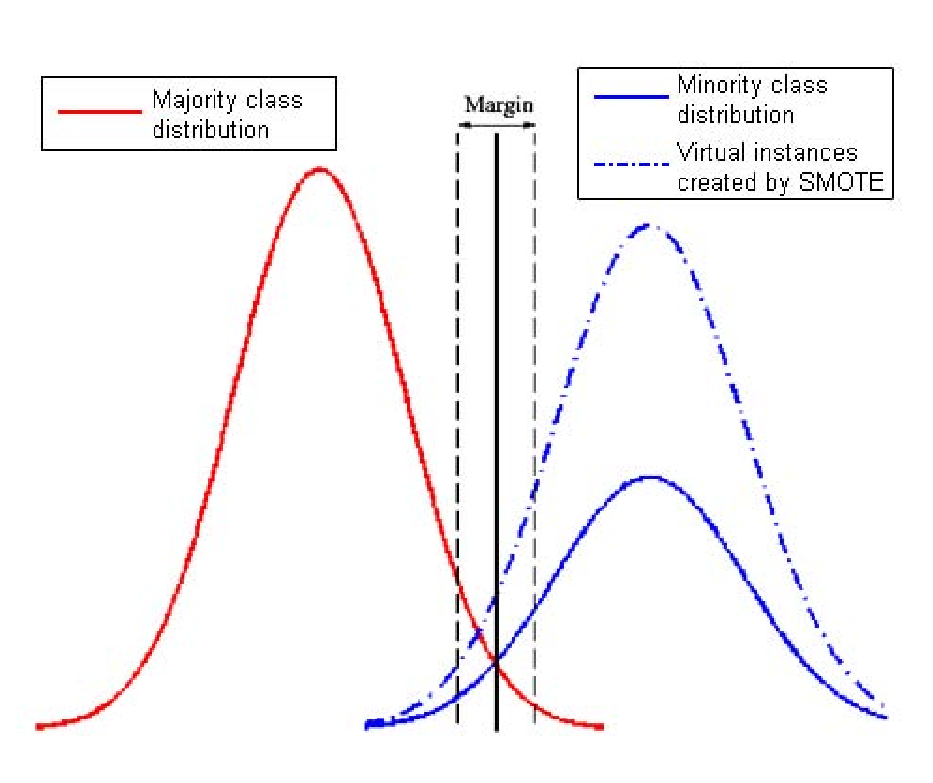
\includegraphics[width=0.45\textwidth, height=4.2cm]{Figures/virtual/smote_proc.eps}
      \label{fig:smote_sample}
      } \quad
      \subfigure[Oversampling with \textsc{Virtual}]{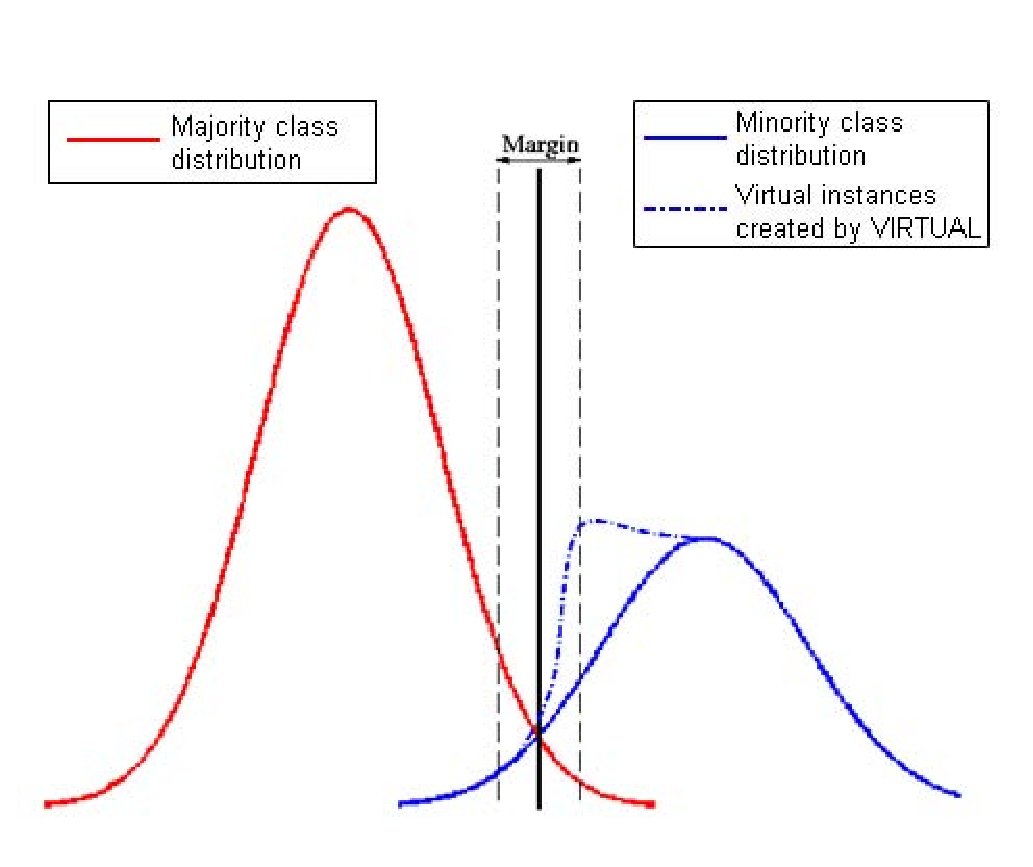
\includegraphics[width=0.45\textwidth, height=4.2cm]{Figures/virtual/virtual_proc.eps}
      \label{fig:virtual_sample}
      }
      }
    \caption{Comparison of oversampling the minority class with SMOTE and VIRTUAL. }
    \label{fig:oversample}
  \end{center}
\end{figure*}

We further analyze the computation complexity of SMOTE and \textsc{Virtual}. The computation complexity of \textsc{Virtual} is $O(\left|SV(+) \right|\cdot v \cdot \mathcal{C})$, where $v$ is the number of virtual instances created for a real positive support vector in each iteration, $\left|SV(+) \right|$ is the number of positive support vectors and $\mathcal{C}$ is the cost of finding k nearest neighbors. The computation complexity of SMOTE is $O(\left| X_R^+\right| \cdot v \cdot \mathcal{C})$, where $\left| X_R^+\right|$ is the number of positive training instances. $\mathcal{C}$ depends on the approach for finding k nearest neighbors. The naive implementation searches all $N$ training instances for the nearest neighbors and thus $\mathcal{C}=kN$. Using advanced data structure such as kd-tree, $\mathcal{C}=k\log N$. Since $\left|SV(+) \right|$ is typically much less than $\left| X_R^+\right|$, \textsc{Virtual} incurs lower computation overhead than SMOTE. Also, with fewer virtual instances created, the learner is less burdened with \textsc{Virtual}. We demonstrate with empirical results that the virtual instances created with \textsc{Virtual} are more informative and the prediction performance is also improved.

\subsection{Experiments}
We conduct a series of experiments on Reuters-21578 and four UCI datasets to demonstrate the efficacy of \textsc{Virtual}. The characteristics of the datasets are detailed in \cite{Ertekin_dissertation}. We compare \textsc{Virtual} with two systems, Active Learning (AL) and SMOTE. AL adopts the traditional active learning strategy without preprocessing or creating any virtual instances during learning. SMOTE, on the other hand, preprocesses the data by creating virtual instances before training and uses random sampling in learning. Experiments elicit the advantages of adaptive virtual sample creation in \textsc{Virtual}.

\begin{figure*}[!t]
  \centering
  \scalebox{1}
  {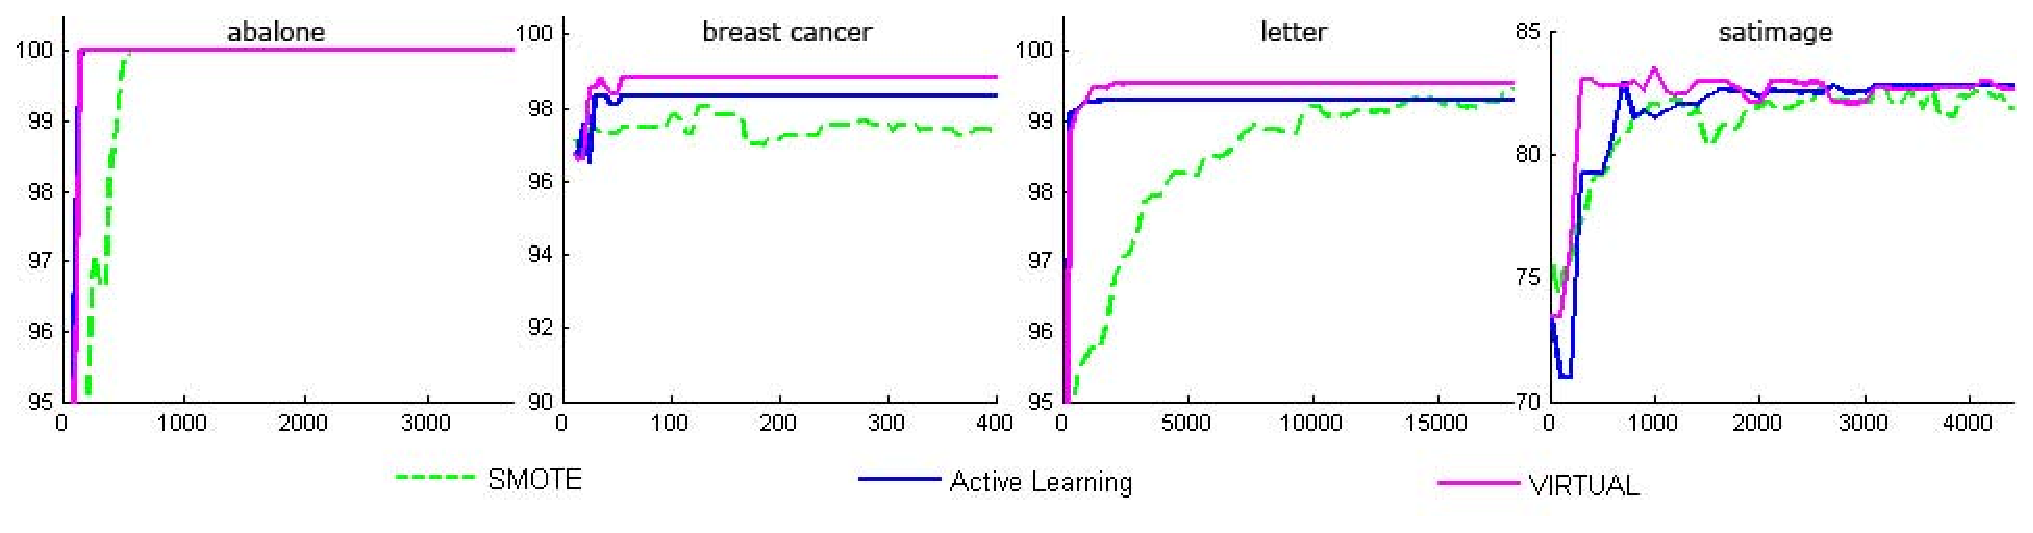
\includegraphics[width=\textwidth]{Figures/virtual/uci-graphs.eps}}\\
  \caption{Comparison of SMOTE, AL and VIRTUAL on \emph{UCI} datasets.
  We present the g-means (\%) (y-axis) of the current model for the test set
  vs. the number of training samples (x-axis) seen.}
  \label{fig:uci}
\end{figure*}


\begin{figure*}[!b]
  \centering
  \scalebox{1}
  {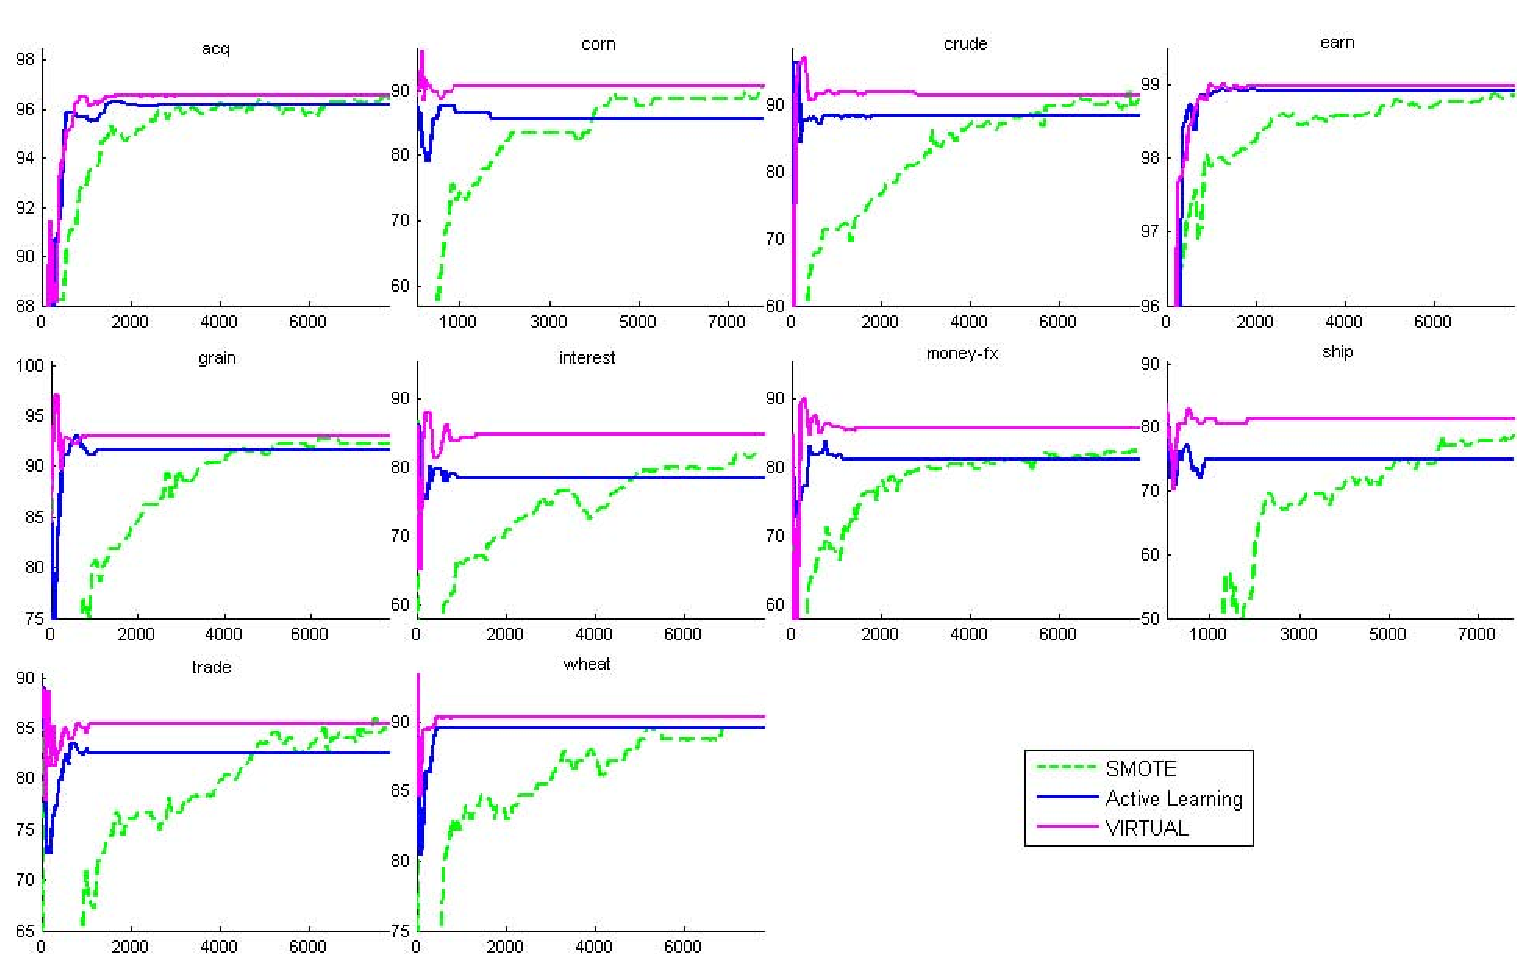
\includegraphics[width=\textwidth]{Figures/virtual/reuters.eps}}\\
  \caption{Comparison of SMOTE, AL and VIRTUAL on 10 largest categories of \emph{Reuters-21578}.
  We show the g-means (\%) (y-axis) of the current model for the test set
  versus the number of training samples (x-axis) seen.}
  \label{fig:reuters}
\end{figure*}


In Figures \ref{fig:uci} and \ref{fig:reuters} provide details on the behavior of the three algorithms, SMOTE, AL and \textsc{Virtual}. For the Reuters datasets (Figure \ref{fig:reuters}), note that in all the 10 categories \textsc{Virtual} outperforms AL in g-means metric after saturation. The difference in performance is most pronounced in the more imbalanced categories, e.g. \emph{corn}, \emph{interest} and \emph{ship}. In the less imbalanced datasets such as \emph{acq} and \emph{earn}, the difference in g-means of both methods is less noticeable. The g-means of SMOTE converges much slower than both AL and \textsc{Virtual}. However, SMOTE converges to higher g-means than AL in some of the categories, indicating that the virtual positive examples provide additional information that can be used to improve the model. \textsc{Virtual} converges to the same or even higher g-means than SMOTE while generating fewer virtual instances. For the UCI datasets (Figure \ref{fig:uci}), \textsc{Virtual} performs as well as AL in \emph{abalone} in g-means and consistently outperforms AL and SMOTE in the other three datasets.

\begin{table}[t!]
\centering \small
\caption{Support vectors with SMOTE (SMT), AL and VIRTUAL. Imb.Rt. is the data imbalance ratio and
\#SV(-)/\#SV(+) represents the support vector imbalance ratio. The rightmost two columns compare the portion of the virtual instances selected as support vectors in SMOTE and VIRTUAL.}
\small
\begin{tabular}{l@{\hspace{1mm}}|l@{\hspace{1mm}}|c@{\hspace{1mm}}|c@{\hspace{1mm}}|c@{\hspace{1mm}}|c@{\hspace{1mm}}|c@{\hspace{1mm}}|c}
\hline
\multicolumn{2}{c|}{\multirow{2}{1cm}{Dataset}}&Imb.&\multicolumn{3}{c|}{\#SV(-)/\#SV(+)}&\multicolumn{2}{c}{\#$SV_V(+)$/\#V.I.}\\\cline{4-8}
\multicolumn{2}{c|}{}&Rt.&SMT&AL&\textsc{Virtual}&SMT&\textsc{Virtual}\\
\hline\hline
\multirow{10}{2mm}{\begin{sideways}\parbox{13mm}{Reuters}\end{sideways}}
&acq&3.7&1.24&1.28&1.18&2.4\%&\textbf{20.3\%}\\
&corn&41.9&2.29&3.08&1.95&17.1\%&\textbf{36.6\%}\\
&crude&19.0&2.30&2.68&2.00&10.8\%&\textbf{50.4\%}\\
&earn&1.7&1.68&1.89&1.67&6.0\%&\textbf{24.2\%}\\
&grain&16.9&2.62&3.06&2.32&7.2\%&\textbf{42.3\%}\\
&interest&21.4&1.84&2.16&1.66&13.3\%&\textbf{72.2\%}\\
&money-fx&13.4&1.86&2.17&1.34&8.2\%&\textbf{31.1\%}\\
&ship&38.4&3.45&4.48&2.80&20.0\%&\textbf{66.5\%}\\
&trade&20.1&1.89&2.26&1.72&15.4\%&\textbf{26.6\%}\\
&wheat&35.7&2.55&3.43&2.22&12.3\%&\textbf{63.9\%}\\
\hline\hline
\multirow{4}{2mm}{\begin{sideways}\parbox{5mm}{UCI}\end{sideways}}
&abalone&9.7&0.99&1.24&0.99&30.4\%&\textbf{69.2\%}\\
&breast&1.9&1.23&0.60&0.64&2.9\%&\textbf{39.5\%}\\
&letter&24.4&1.21&1.48&0.97&0.98\%&\textbf{74.4\%}\\
&satimage&9.7&1.31&1.93&0.92&37.3\%&\textbf{53.8\%}\\
\hline
\end{tabular}
\label{tbl:res_svs}
\end{table}

In Table \ref{tbl:res_svs}, the support vector imbalance ratio of all the three methods are lower than the data imbalance ratio, and \textsc{Virtual} achieves the most balanced ratios of positive and negative support vectors in the Reuters datasets. Despite that the datasets used have different data distributions, the portion of virtual instances which become support vectors in \textsc{Virtual} consistently and significantly higher than that in SMOTE. These results confirm the previous discussion that \textsc{Virtual} is more effective in generating informative virtual instances.

Table \ref{tbl:res_all} presents g-means and the total learning time for SMOTE, AL and  \textsc{Virtual}. Classical batch SVM's g-means values are also provided as a reference point. In Reuters datasets, \textsc{Virtual} yields the highest g-means in all categories. Table 4 shows the effectiveness of adaptive virtual instance generation. In categories \emph{corn}, \emph{interest} and \emph{ship} with high class imbalance ratio, \textsc{Virtual} gains substantial improvement in g-means. Compared to AL, \textsc{Virtual} requires additional time for the creation of virtual instances and selection of those which may become support vectors. Despite this overhead, \textsc{Virtual}'s training times are comparable with that of AL. In the cases where minority examples are abundant, SMOTE demands substantially longer time to create virtual instances than \textsc{Virtual}. But as the rightmost columns in Table 3 show, only a small fraction of the virtual instances created by SMOTE become support vectors. Therefore SMOTE spends much time to create virtual instances that will not be used in the model. On the other hand, \textsc{Virtual} has already a short training time and uses this time to create more informative virtual instances. In Table 4, the numbers in parentheses give the ranks of the g-means prediction performance of the four approaches. The values in bold correspond to a win and \textsc{Virtual} wins in nearly all datasets.  The Wilcoxon signed-rank test (2-tailed) between \textsc{Virtual} and its nearest competitor SMOTE reveals that the zero median hypothesis can be rejected at the significance level 1\% ($p=4.82 \times 10^{-4}$), implying that \textsc{Virtual} performs statistically better than SMOTE in these 14 datasets. These results demonstrate the importance of creating synthetic samples from the informative examples rather than all the examples.


\begin{table*}[!tp]\centering \small
\caption{g-means and total learning time using SMOTE, AL and VIRTUAL.
`Batch' corresponds to the classical SVM learning in batch setting without resampling.
The numbers in brackets denote the rank of the corresponding method in the dataset.}
\begin{tabular}{l|l|c@{\hspace{1mm}}|c@{\hspace{1mm}}|c@{\hspace{1mm}}|c@{\hspace{1mm}}|c|r|c}
\hline
\multicolumn{2}{c|}{\multirow{2}{1cm}{Dataset}}&\multicolumn{4}{c|}{g-means (\%)}&\multicolumn{3}{c}{Total learning time (sec.)}\\\cline{3-9}
\multicolumn{2}{c|}{}&Batch&SMOTE&AL&\textsc{Virtual}&SMOTE&AL&\textsc{Virtual}\\
\hline\hline
\multirow{10}{3mm}{\begin{sideways}\parbox{13mm}{Reuters}\end{sideways}}
&acq&96.19 (3)&96.21 (2)&96.19 (3)&\textbf{96.54 (1)}&2271&146&203\\
&corn&85.55 (4)&89.62 (2)&86.59 (3)&\textbf{90.60 (1)}&74&43&66\\
&crude&88.34 (4)&91.21 (2)&88.35 (3)&\textbf{91.74 (1)}&238&113&129\\
&earn&98.92 (3)&\textbf{98.97 (1)}&98.92 (3)&\textbf{98.97 (1)}&4082&121&163\\
&grain&91.56 (4)&92.29 (2)&91.56 (4)&\textbf{93.00 (1)}&296&134&143\\
&interest&78.45 (4)&83.96 (2)&78.45 (4)&\textbf{84.75 (1)}&192&153&178\\
&money-fx&81.43 (3)&83.70 (2)&81.08 (4)&\textbf{85.61 (1)}&363&93&116\\
&ship&75.66 (3)&78.55 (2)&74.92 (4)&\textbf{81.34 (1)}&88&75&76\\
&trade&82.52 (3)&84.52 (2)&82.52 (3)&\textbf{85.48 (1)}&292&72&131\\
&wheat&89.54 (3)&89.50 (4)&89.55 (2)&\textbf{90.27 (1)}&64&29&48\\
\hline\hline
\multirow{4}{2mm}{\begin{sideways}\parbox{5mm}{UCI}\end{sideways}}
&abalone&\textbf{100 (1)}&\textbf{100 (1)}&\textbf{100 (1)}&\textbf{100 (1)}&18&4&6\\
&breast&98.33 (2)&97.52 (4)&98.33 (2)&\textbf{98.84 (1)}&4&1&1\\
&letter&99.28 (3)&99.42 (2)&99.28 (3)&\textbf{99.54 (1)}&83&5&6\\
&satimage&\textbf{83.57 (1)}&82.61 (4)&82.76 (3)&82.92 (2)&219&18&17\\
\hline
\end{tabular}
\vspace{-3mm}
\label{tbl:res_all}
\end{table*}

\drop{
\section{Conclusions}
The class imbalance problem has been known to hinder the generalization performance of classification algorithms. This chapter offers a better understanding of how active learning can remedy the problems that stem from class imbalance and presents techniques to improve the efficiency of active learning when dealing with such problems.

This chapter begins by  first present an efficient active learning method which selects informative instances from a randomly picked small pool of examples rather than making a full search in the entire training set. This strategy renders active learning to be applicable to very large datasets which otherwise would be computationally very expensive. Combined with the early stopping heuristics, active learning achieves a fast and scalable solution without sacrificing prediction performance. We then show that this active learning strategy can be used to address the class imbalance problem. In simulation studies, we demonstrate that as the imbalance ratio increases, active learning can achieve better prediction performance than random sampling by only using the informative portion of the training set. By focusing the learning on the instances around the classification boundary, more balanced class distributions can be provided to the learner in the earlier steps of the learning.  Our empirical results on a variety of real-world datasets allow us to conclude that active learning is comparable or even better than other popular resampling methods in dealing with imbalanced data classification.

The second part presents an active learning based adaptive resampling strategy, \textsc{Virtual} to address the imbalanced data classification problem in SVMs. \textsc{Virtual} adaptively creates instances according to the real positive support vectors selected in each active learning step. These instances are informative as they are close to the hyperplane. Thus \textsc{Virtual} creates fewer virtual instances that are informative. Our complexity analysis shows that \textsc{Virtual} incurs lower overhead in data generation and eventually less burden to the learner. Our thorough empirical results on both artificial and real-world data demonstrate that \textsc{Virtual} is capable of
achieving higher g-means than active learning without oversampling (AL) and SMOTE. Experimental results also show that \textsc{Virtual} is more resilient to high class imbalance ratios due to its capability of creating more balanced models using the virtual instances created. The training time of \textsc{Virtual} is substantially shorter than SMOTE in most cases.
}

%\section{Active Learning for Imbalanced Data Classification}
\label{al_for_imbalanced_data}
As we outlined in Section~\ref{sec:background}, active learning is primarily considered as a technique to reduce the number of training samples that need to be labeled for a classification task. From a traditional perspective, the active learner has access to a vast pool of unlabeled examples, and it aims to make a clever choice to select the most informative example to obtain its label. However, even in the cases where the labels of training data are already available, active learning can still be leveraged to obtain the informative examples through training sets \cite{Schohn_2000,Bordes_2005,Huang_2006}. For example, in large-margin classifiers such as Support Vector Machines (SVM), the \textit{informativeness} of an example is synonymous with its distance to the hyperplane. The farther an example is to the hyperplane, the more the learner is confident about its true class label, hence there is little, if any, benefit that the learner can gain by asking for the label of that example. On the other hand, the examples close to the hyperplane are the ones that yield the most information to the learner. Therefore, the most commonly used active learning strategy in SVMs is to check the distance of each unlabeled example to the hyperplane and focus on the examples that lie closest to the hyperplane, as they are considered to be the most informative examples to the learner.

\begin{figure}[t!]
    \centering
        \scalebox{0.5}{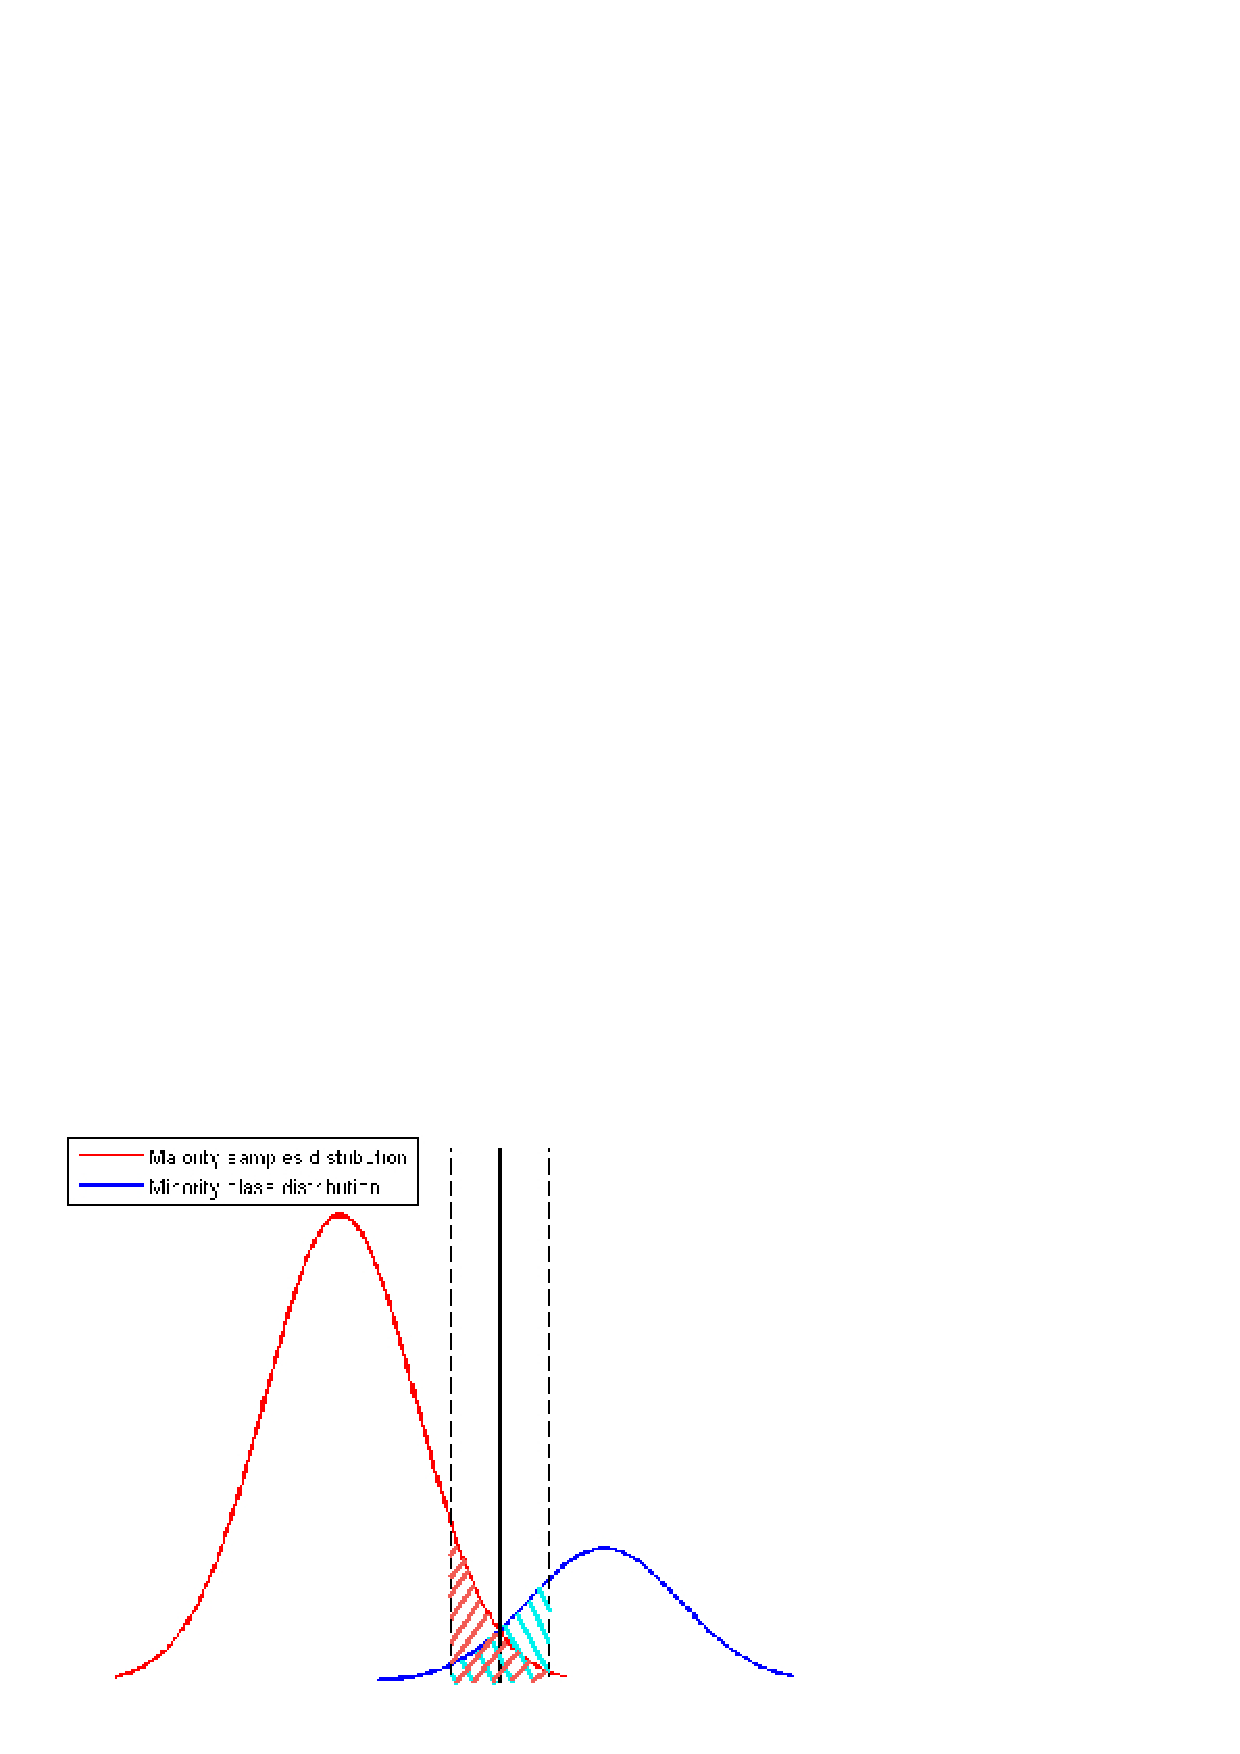
\includegraphics{Figures/lotb/al-imb-shade.pdf}}
    \caption{Data within the margin is less imbalanced than the entire data.}
    \label{fig:alimbshade}
\end{figure}

The strategy of selecting examples within the margin also strongly addresses the problems that arise from imbalanced classes. Suppose that the class distributions of an imbalanced dataset is given in Figure \ref{fig:alimbshade}. The shaded region corresponds to the class distribution of the data within the margin. As shown in the figure, the imbalance ratio of the classes within the margin is much smaller than the class imbalance ratio of the entire dataset. Therefore, any selection strategy that focuses on the examples in the margin most likely ends up with a more balanced class distribution than that of the entire dataset. Our empirical findings with various type of real-world data confirm that the imbalance ratios of the classes within the margin in real-world data are generally much lower than that of the entire data.

In this section, we constrain our discussion to standard two-class classification problems with Support Vector Machines (SVMs). The next section presents a brief overview of SVMs, followed by the working principles of an efficient active learning algorithm in Section \ref{ALpools}. We explain the advantage of using online SVMs with the active sample selection in Section \ref{LASVM}. In Section \ref{ES}, we then describe an early stopping heuristics for active learning.

\subsection{Support Vector Machines}
\label{SVMs}
Support Vector Machines \cite{Vapnik_1995} are well known for their strong theoretical foundations, generalization performance and ability to handle high dimensional data. In the binary classification setting, let $((x_{1}, y_{1})\cdots(x_{n}, y_{n}))$ be the training dataset where $x_i$ are the feature vectors representing the instances and  $y_i \in (-1,+1)$ be the labels of the instances.  Using the training set, SVM builds an optimum hyperplane -- a linear discriminant in a higher dimensional feature space -- that separates the two classes by the largest margin. This hyperplane is obtained by minimizing the following objective function:
\begin{equation}
\label{svm_primal}
\min_{{\bf{w}, b, \xi_{i}}}\frac{1}{2} {\bf w\cdot w}^T + C\sum_{i=1}^{N}\xi_i  \\
\end{equation}
\begin{equation}
\mbox{subject to}\left\{ \begin{array}{l} \forall i \; y_i({\bf
w}^T{\Phi(x_i)} - b)\geq 1-\xi_{i}\\ \forall i \; \xi_{i} \geq 0
\end{array} \right.
\end{equation}
where \textbf{w} is the norm of the hyperplane, $b$ is the  offset, $y_i$ are the labels, $\Phi(\cdot)$ is the mapping from input space to feature space, and $\xi_i$ are the slack variables that permit the non-separable case by allowing misclassification of training instances. In practice the convex quadratic programming (QP) problem in (\ref{svm_primal}) is solved by optimizing the dual cost function. The dual representation of (\ref{svm_primal}) is given as
\begin{equation}
\label{svm_dual}
\max W(\alpha) \equiv \sum_{i=1}^{N}\alpha_{i} - \frac{1}{2}\sum_{i,j}\alpha_i\alpha_{j}y_{i}y_{j}K({\bf x_i},{\bf x_j}) \\
\end{equation}
\begin{equation}
\mbox{subject to}\left\{ \begin{array}{l} \forall i\; 0 \leq \alpha_i \leq C\\ \sum_{i=1}^{N}\alpha_i y_i=0 \end{array} \right.
\end{equation}
where $y_i$ are the labels, $\Phi(\cdot)$ is the mapping from the input space to the feature space, $K({\bf x_i}, {\bf x_j})=\langle\Phi({\bf x_i}),\Phi({\bf x_j})\rangle$ is the kernel matrix and the $\alpha_i$'s are the \textit{Lagrange multipliers} which are non-zero only for the training instances which fall in the margin. Those training instances are called \textit{support vectors} and they define the position of the hyperplane. After solving the QP problem, the norm of the hyperplane \textbf{w} can be represented as
\begin{equation}
\label{svm_norm}
\textbf{w}=\sum_{i=1}^{n}\alpha_i\Phi(x_i)
\end{equation}

\subsection{Margin-based Active Learning with SVMs}
\label{ALpools}
Note that in (\ref{svm_norm}), only the support vectors affect the SVM solution. This means that if SVM is retrained with a new set of data which only consist of those support vectors, the learner will end up finding the same hyperplane. This emphasizes the fact that not all examples are equally important in training sets. Then the question becomes how to select the most informative examples for labeling from the set of unlabeled training examples. This section focuses on a form of selection strategy called \textit{margin-based active learning}. As we highlighted earlier, in SVMs the most informative example is believed to be the closest one to the hyperplane since it divides the \textit{version space} into two equal parts. The aim is to reduce the version space as fast as possible to reach the solution faster in order to avoid certain \textit{costs} associated with the problem. For the possibility of a non-symmetric version space, there are more complex selection methods suggested by \cite{Tong_2002}, but it has been observed that the advantage of those are not significant, considering their high computational costs.

\textbf{Active Learning with Small Pools:}
 The basic working principle of margin-based active learning with SVMs is: $i)$ train an SVM on the existing training data, $ii)$ select the closest example to the hyperplane, and $iii)$ add the new selected example to the training set and train again. In classical active learning \cite{Tong_2002}, the search for the most informative example is performed over the entire dataset. Note that, each iteration of active learning involves the recomputation of each training example's distance to the new hyperplane. Therefore, for large datasets, searching the entire training set is a very time consuming and computationally expensive task.

One possible remedy for this performance bottleneck is to use the ``59 trick'' \cite{Smola_2000}, which does not necessitate a full search through the entire dataset but locates an approximate most informative sample by examining a small constant number of randomly chosen samples. The method picks $L$ ($L \ll$ \# training examples) random training samples in each iteration and selects the best (closest to the hyperplane) among them. Suppose, instead of picking the closest example among all the training samples $X_N=(x_1, x_2, \cdots ,x_N)$ at each iteration, we first pick a random subset $X_L$, $L\ll N$ and select the closest sample $x_i$ from $X_L$ based on the condition that $x_i$ is among the top $p\%$ closest instances in $X_N$ with probability $(1-\eta)$. Any numerical modification to these constraints can be met by varying the size of $L$, and is independent of $N$. To demonstrate, the probability that at least one of the $L$ instances is among the closest $p\%$ is $1-(1-p\%)^L$. Due to the requirement of $(1-\eta)$ probability, we have
\begin{equation}
1-(1-p\%)^L = 1-\eta
\end{equation}
which follows the solution of $L$ in terms of $\eta$ and $p$
\begin{equation}
L={{\log \eta} \;/\;{\log(1-p\%)}}
\end{equation}
For example, the active learner will pick one example, with $95\%$ probability, that is among the top $5\%$ closest instances to the hyperplane, by randomly sampling only $\lceil \log(.05)/\log(.95) \rceil = 59$ examples regardless of the training set size. This approach scales well since the size of the subset $L$ is independent of  the training set size $N$, requires significantly less training time and does not have an adverse effect on the classification performance of the learner.

\begin{figure*}[t]
    \centering
        \scalebox{0.34}{\includegraphics{Figures/lotb/rpal.pdf}}
    \caption{Comparison of PRBEP and g-means of RS, AL(full search) and AL(random pool). The training times of AL(full search) vs. AL(random pool) until saturation in seconds are: 272 vs. 50 (grain), 142 vs. 32 (ship) and 126 vs. 13 (USPS). AL(random pool) is 4 to 10 times faster than AL(full search) with similar prediction performance.}
    \label{fig:rpal}
\end{figure*}

Figure \ref{fig:rpal} shows the comparisons of PRBEP and g-means performances of AL(random pool) and the traditional active learning method AL(full search) \cite{Tong_2002}. For the random pool strategy, we set $L=59$ which means we pick 59 random examples to form the query pool  at each learning step and pick the closest example to the hyperplane from this pool. RS corresponds to the random sampling strategy where the examples are selected randomly. As Figure \ref{fig:rpal} depicts, active learning method with small pools achieves as good prediction performance as the traditional active learning method. Moreover, the random pool strategy is 4 to 10 times faster than traditional active learning for the given datasets.

\subsection{Online SVM for Active Learning}
\label{LASVM}
Online learning algorithms are usually associated with problems where the complete training set is not available. However, in cases where the complete training set is available, their computational properties can be leveraged for faster classification and incremental learning. In our framework, we use an online SVM algorithm, LASVM \cite{Bordes_2005} instead of a traditional batch SVM tool (e.g., libsvm, SVM\textsuperscript{\textit{light}}). LASVM is an online kernel classifier which relies on the traditional soft margin SVM formulation. LASVM yields the classification accuracy rates of the state-of-the art traditional SVM solvers but requires less computational resources. Traditional SVM works in a batch setting where all the training instances are used to form the one and final model. LASVM, on the other hand, works in an online setting, where its model is continually modified as it processes training instances one by one. Each LASVM iteration receives a fresh training example and tries to optimize the dual cost function in Equation (\ref{svm_dual}) using feasible direction searches.
They can select a new data to process either by random or active selection and can integrate the information of the new seen data to the system without training on all the samples again, hence they can incrementally build a learner. This working principle of online learning algorithms leads to speed improvement and less memory demand which makes the algorithm applicable to very large datasets. More importantly, this incremental working principle suits the nature of active learning in a much better way than the batch algorithms. Empirical evidence indicates that a single presentation of each training example to the algorithm is sufficient to achieve training errors comparable to those achieved by the SVM solution \cite{Bordes_2005}. In section \ref{ES} we also show that if we use an early stopping criteria in active sample selection, we do not have to introduce all training examples to the learner.

\subsection{Active Learning with Early Stopping}
\label{ES}
Early stopping criteria is advantageous to active learning since it converges to the solution faster than the random sample selection method. A theoretically sound method to stop training is when the examples in the margin are exhausted. To check if there are still unseen training examples in the margin, the distance of the new selected example is compared against the support vectors of the current model. If the new selected example by active learning (closest to the hyperplane) is not closer than any of the support vectors, we conclude that the margin is exhausted. A practical implementation of this idea is to count the number of support vectors during the active learning training process. If the number of the support vectors stabilizes, it implies that all possible support vectors have been selected by the active learning method.

\begin{figure}[b]
    \hspace{-10mm}
        \scalebox{0.3}{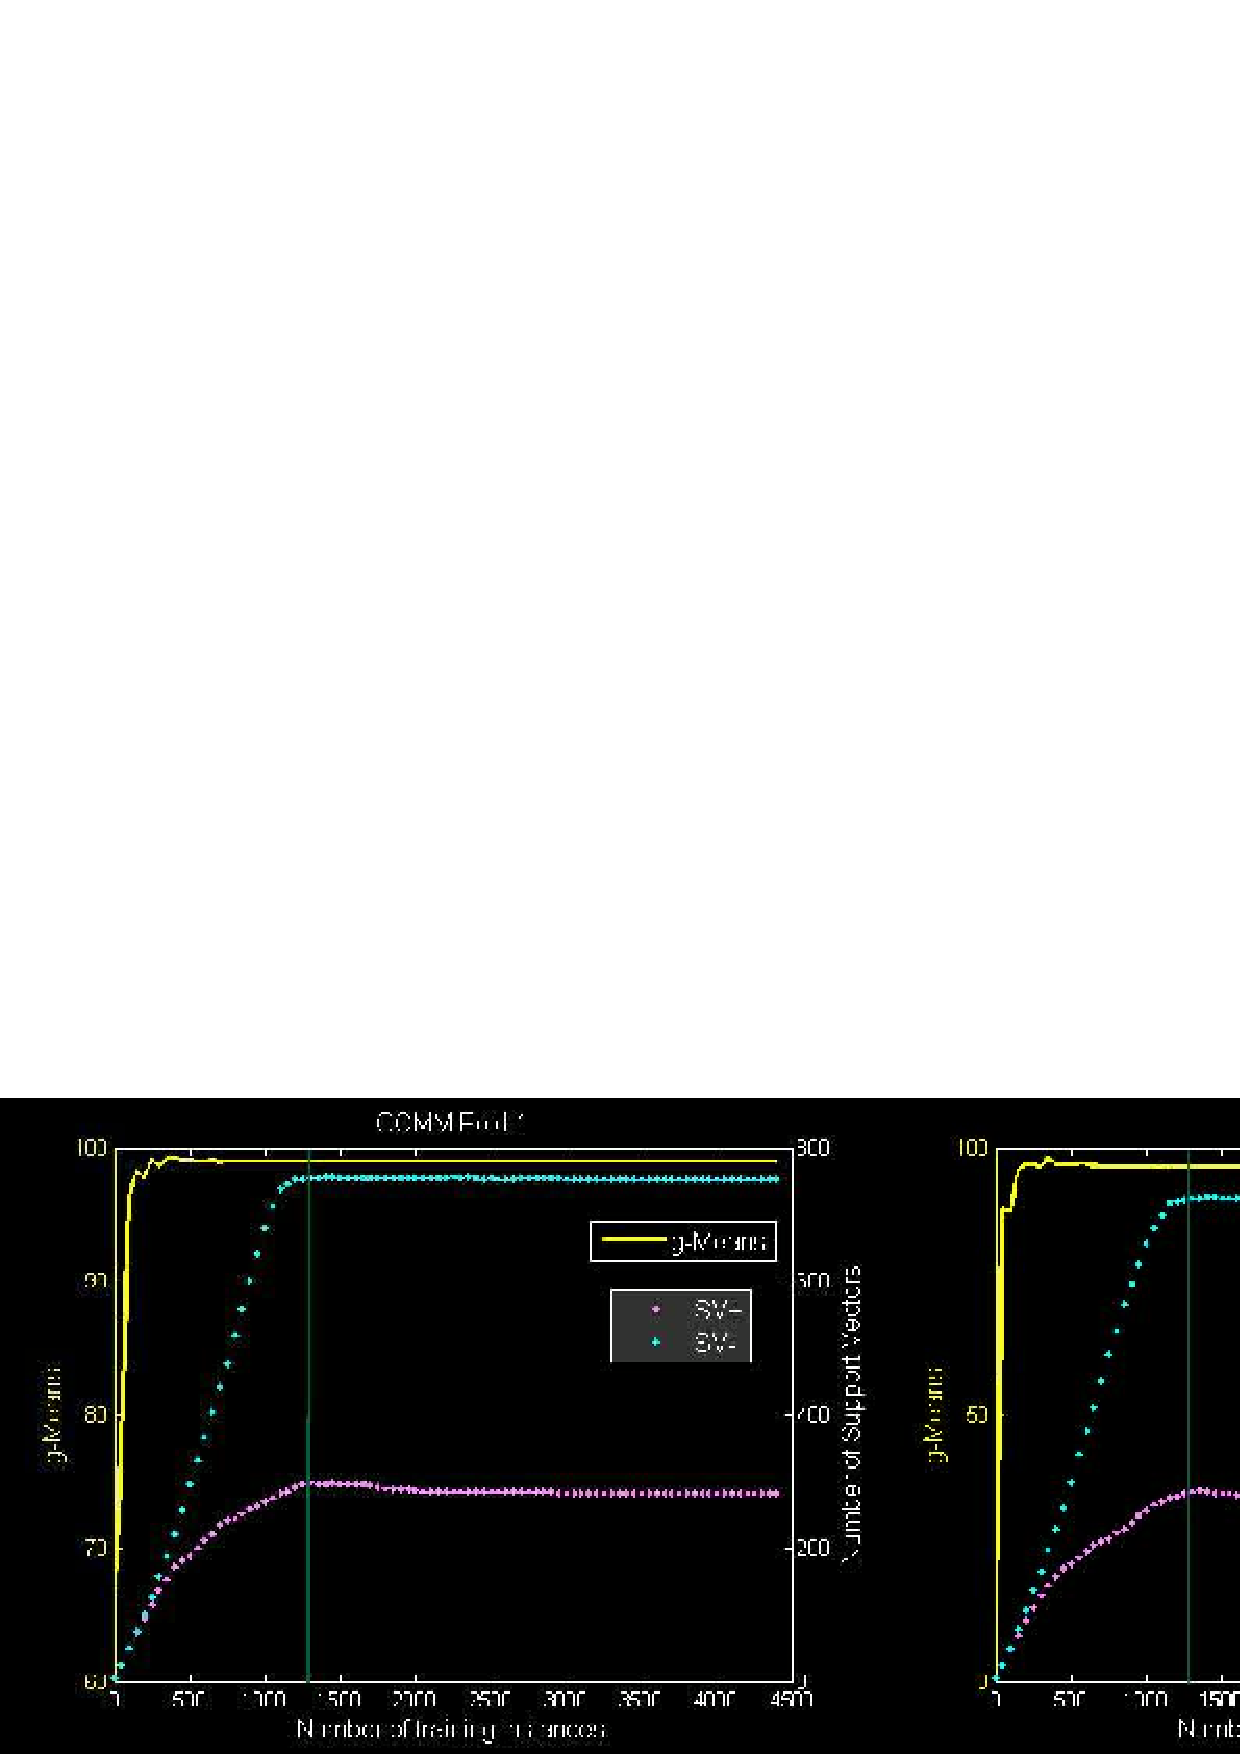
\includegraphics{Figures/lotb/comm.pdf}}
    \caption{3-fold cross-validation results for the training set of the category COMM in CiteSeer dataset. Vertical lines correspond to early stopping points.}
    \label{fig:comm}
\end{figure}

In order to analyze this method, we conducted a 3-fold cross-validation on one of the datasets (see Figure \ref{fig:comm}). In cross-validation, $2/3$ of the training set is used for training and the remaining $1/3$ is reserved as the hold-out dataset. Since the training set distribution is representative of the test set distribution, we believe that the algorithm's behavior would most likely be the same in the test set. As can be seen in Figure \ref{fig:comm}, in active learning setups, after using certain number of labeled training data, the number of support vectors saturates and  g-means levels off as well. Those graphs support the idea that the model does not change after the system observes enough informative samples. Further, adding more training data after this point does not make a remarkable change in the model and consequently in prediction performance. Notice that in Figure \ref{fig:comm} the vertical line indicates the suggested early stopping point and it is approximately equal in all three folds. As a result, we adopt the early stopping strategy of examining the number of support vectors in the entire training datasets without performing cross-validation.

\subsection{Performance Metrics}
Classification accuracy is not a good metric to evaluate classifiers in applications with class imbalance problem.  SVMs have to achieve a tradeoff between maximizing the margin and minimizing the empirical error. In the non-separable case, if the misclassification penalty $C$ is very small, SVM learner simply tends to classify every example as negative. This extreme approach makes the \textit{margin} the largest while making no classification errors on the negative instances. The only error is the cumulative error of the positive instances which are already few in numbers. Considering an imbalance ratio of 99 to 1, a classifier that classifies everything as negative, will be 99\% accurate but it will not have any practical use as it can not identify the positive instances.

For the evaluation of our results, we use several other prediction performance metrics such as g-means, AUC and PRBEP which are commonly used in imbalanced data classification. g-means \cite{Kubat_1997} is denoted as $g=\sqrt{sensitivity \cdot specificity}$ where sensitivity is the accuracy on the positive instances given as $True Pos./(True Pos.+False Neg.)$ and specificity is the accuracy on the negative instances given as $True Neg./(True Neg.+False Pos.)$.

The Receiver Operating Curve (ROC) displays the relationship between sensitivity and specificity at all possible thresholds for a binary classification scoring model, when applied to independent test data. In other words, ROC curve is a plot of the true positive rate against the false positive rate as the decision threshold is changed. The \textit{area under the ROC curve} (AUC) is a numerical measure of a model's discrimination performance and shows how successfully and correctly the model separates the positive and negative observations and ranks them. Since AUC metric evaluates the classifier across the entire range of decision thresholds, it gives a good overview about the performance when the operating condition for the classifier is unknown or the classifier is expected to be used in situations with significantly different class distributions.

Precision Recall Break-Even Point (PRBEP) is another commonly used performance metric for imbalanced data classification. PRBEP is the accuracy of the positive class at the threshold where precision equals to recall. Precision is defined as $True Pos./(True Pos.+False Pos.)$ and recall is defined as $True Pos./(True Pos.+False Neg.)$


\begin{table}[t!]
\caption{Overview of the datasets.} \centering \small
\begin{tabular}{l|l|r@{\hspace{2mm}}r@{\hspace{2mm}}r@{\hspace{2mm}}r|c c}
\hline
\multicolumn{2}{c|}{Dataset}&\#Feat.&\#Pos&\#Neg&Ratio&c&$\gamma$\\
\hline\hline
\multirow{5}{5mm}{\begin{sideways}\parbox{13mm}{Reuters}\end{sideways}}&Crude&8315&389&7381&19.0&2&1\\
&Grain&8315&433&7337&16.9&2&1\\
&Interest& 8315 &347&7423&21.4&1&2\\
&Money-fx& 8315 &538&7232&13.4&1&0.5\\
&Ship& 8315 &197&7573&38.4&1&0.5\\
&Wheat& 8315 &212&7558&35.7&1&0.5\\
\hline
\multirow{5}{5mm}{\begin{sideways}\parbox{12mm}{CiteSeer}\end{sideways}}
&AI& 6946 &1420&5353&4.3&50&0.1\\
&COMM& 6946 &1252&5341&4.2&50&0.1\\
&Crypt& 6946 &552&6041&11.0&50&0.1\\
&DB& 6946 &819&5775&7.1&50&0.1\\
&OS& 6946 &262&6331&24.2&50&0.1\\
\hline
\multirow{2}{5mm}{\begin{sideways}\parbox{8mm}{UCI}\end{sideways}}
&Abalone-7& 9 &352&3407&9.7&100&0.01\\
&Letter-A&16 &710&17290&24.4&10&0.01\\
&Satimage&36&415&4020&9.69&50&0.001\\
\hline
\multicolumn{2}{c|}{USPS}& 256 &1232&6097&5.0&1000&2\\
\hline
\multicolumn{2}{c|}{MNIST-8}& 780 &5851&54149&9.3&1000&0.02\\
\hline
\end{tabular}
\label{tbl:overview}
\end{table}

\subsection{Datasets}
We study the performance of the algorithm on various benchmark real-world datasets. The overview of the datasets are given in Table \ref{tbl:overview}. The \emph{Reuters-21578} is a popular text mining benchmark dataset. We test the algorithms with 8 of the top 10 most populated categories of \emph{Reuters-21578}. We did not use categories `earn' and `acq' since their class imbalance ratios are not high enough. As a text dataset, we also used 5 categories from CiteSeer\footnote{http://citeseer.ist.psu.edu} data. We used 4 benchmark datasets from the popular UCI Machine Learning Repository as well. \emph{Letter} and \emph{satimage} are image datasets. The `letter A' is used as the positive class in \emph{letter} and `class 4' (damp grey soil) is used as positive class in \emph{satimage}. \emph{Abalone} is a biology dataset where the instances labeled as `class 7' are used to form the positive class. \emph{MNIST} and \emph{USPS} are OCR data of handwritten digits and `digit 8' is used as a positive class in \emph{Mnist}. \emph{Adult} is a census dataset to predict if the income of a person is greater than 50K based on several census parameters, such as age, education, marital status etc. The training set consists of 32,562 instances and the class imbalance ratio is 3. \emph{Waveform} is a popular artificial dataset used commonly in simulation studies. These datasets cover a wide range of data imbalance ratios.

\subsection{Experiments and Empirical Evaluation}
\label{lotb_experiments}
We first conduct experiments to compare the performance of AL(random pool) strategy with the traditional active learning method, AL(full search). The results show that with the proposed method, we can make faster active learning without sacrificing any prediction performance (see Figure \ref{fig:rpal}). In the rest of the section, we refer to AL(random pool) as AL since it is the only active learning method that we used afterwards.

\begin{figure}[b!]
        \scalebox{0.47}{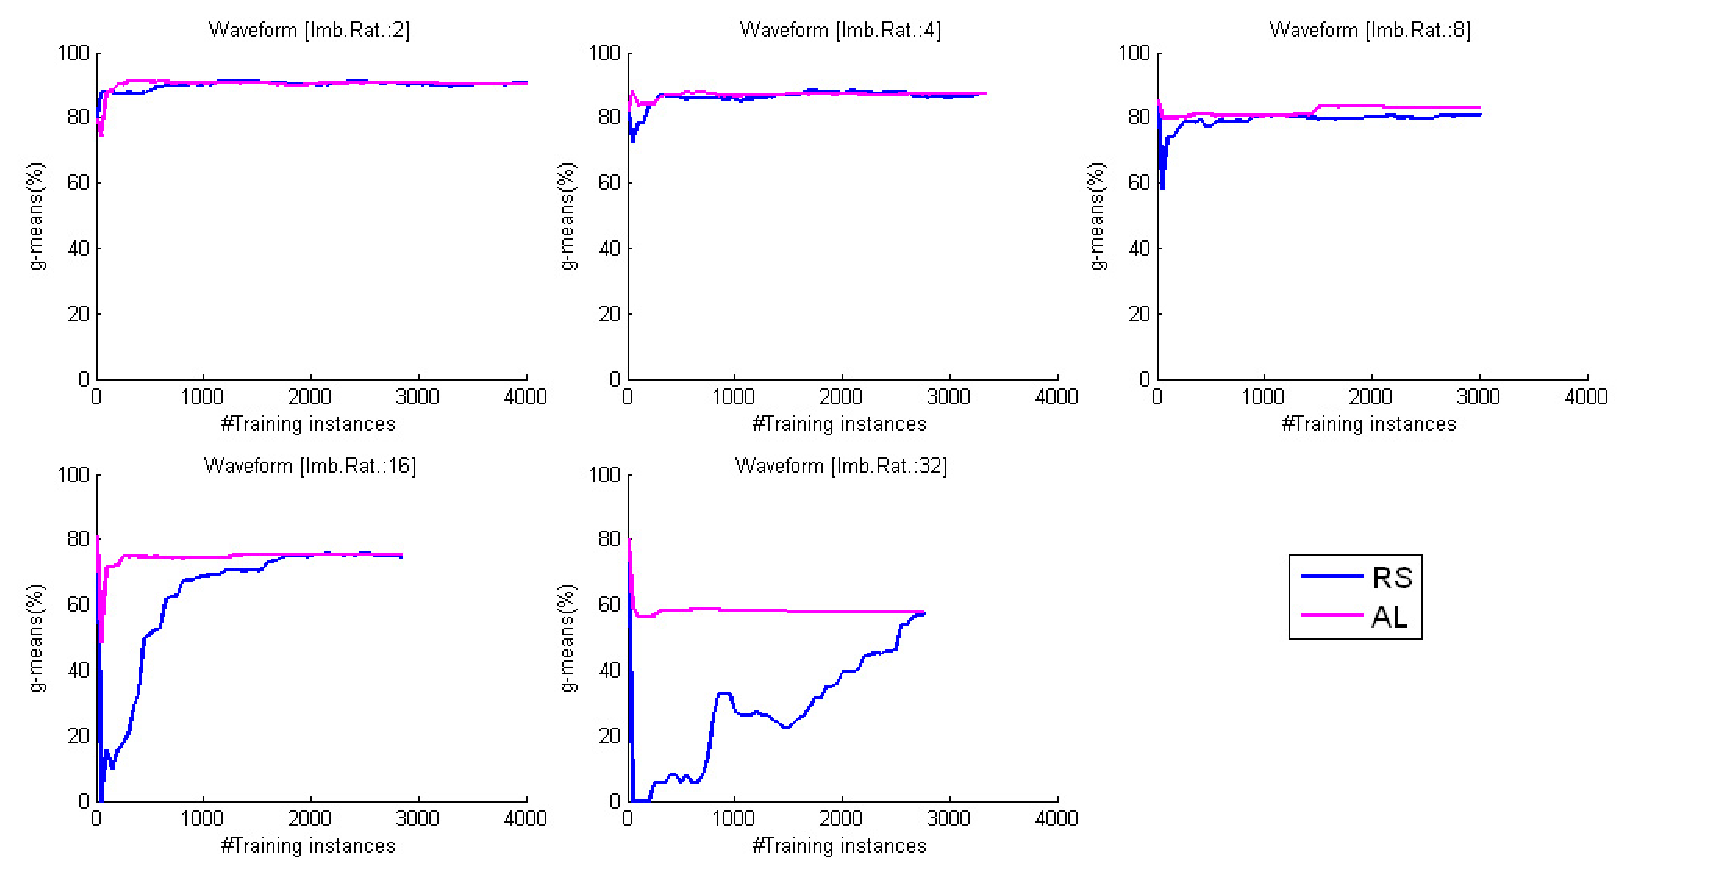
\includegraphics{Figures/lotb/wfall.eps}}
    \caption{Comparison of g-means of AL and RS on the waveform datasets with different imbalance ratios (Imb.R.=2, 4, 8, 16, 32).}
    \label{fig:wfall}
\end{figure}
\begin{figure}[bh!]
\begin{center}
\vspace{-4mm}
\subfigure {
\includegraphics[width=55mm]{Figures/lotb/adultall_1.jpg}
}
\subfigure {
\includegraphics[width=55mm]{Figures/lotb/adultall_2.jpg}
}\\
\vspace{-2mm}
\subfigure {
\includegraphics[width=55mm]{Figures/lotb/adultall_3.jpg}
}
\subfigure {
\includegraphics[width=55mm]{Figures/lotb/adultall_4.jpg}
}
 \caption{Comparison of PRBEP of AL and RS on the adult datasets with different imbalance ratios (Imb.R.=3, 10, 20, 30).}
    \label{fig:adultall}
\end{center}
\end{figure}


In order to make a thorough analysis on the effect of AL to imbalanced data classification, we examine its performance by varying class imbalance ratios using two performance metrics. We randomly remove the examples from the minority class in \emph{Waveform} and \emph{Adult} datasets to achieve different data imbalance ratios. Comparisons of g-means of AL and RS in Figure \ref{fig:wfall} show that the prediction performance of AL is less sensitive to the class imbalance ratio changes than that of the RS. Comparisons of another performance metric PRBEP in Figure \ref{fig:adultall} give even more interesting results. As the class imbalance ratio is increased, AL curves display peaks in the early steps of the learning. This implies that by using an early stopping criteria AL can give higher prediction performance than RS can possibly achieve even after using all the training data. Figure \ref{fig:adultall} curves allow us to think that addition of any instances to the learning model after finding the informative instances can be detrimental to the prediction performance of the classifier. This finding strengthens the idea of applying an early stopping to active learning algorithms.

\begin{figure}[t!]
        \scalebox{0.3}{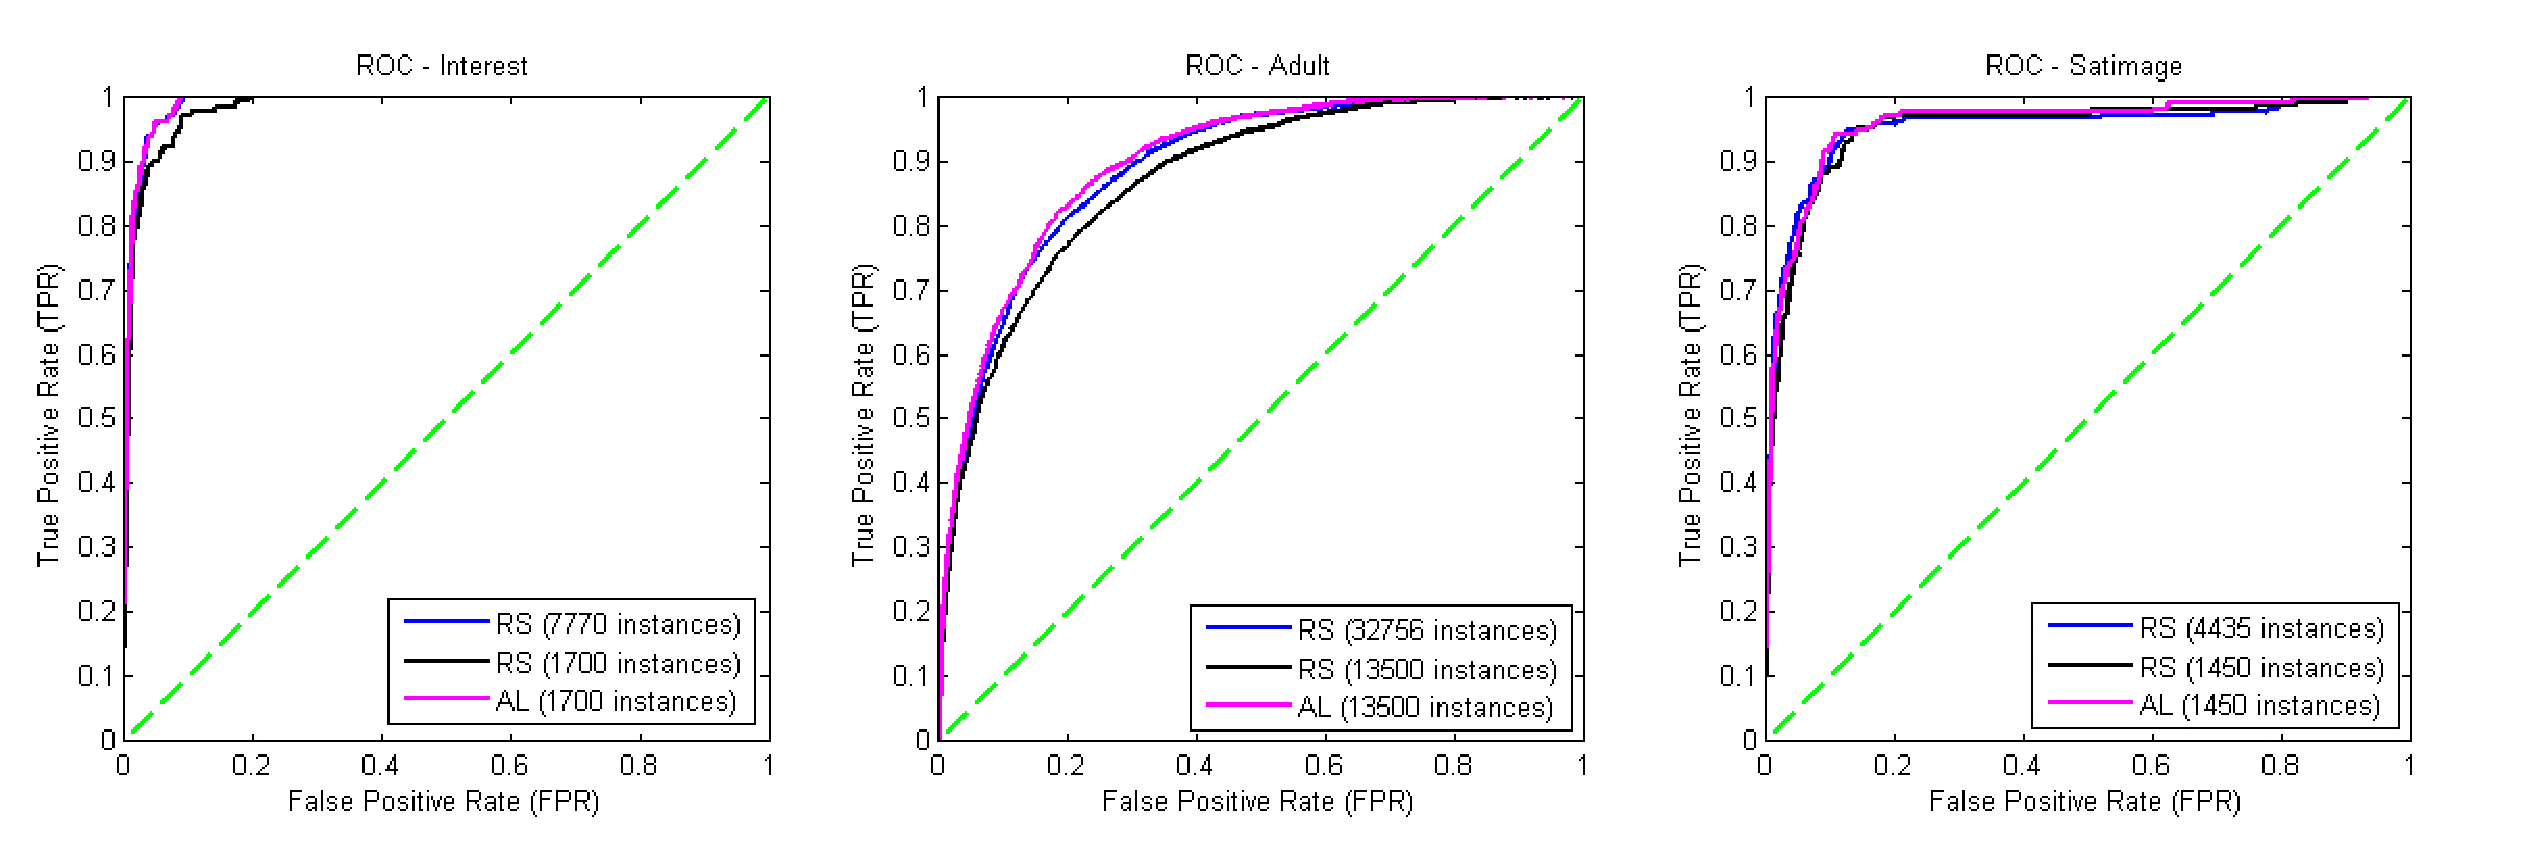
\includegraphics{Figures/lotb/rocall.eps}}
    \caption{Comparison of ROC curves of AL, RS (early stopped at the same number of instances as AL) and RS (with all training data) in Interest, Adult and Satimage datasets.}
    \label{fig:rocall}
\end{figure}
\begin{figure}[b!]
    \centering
        \scalebox{0.45}{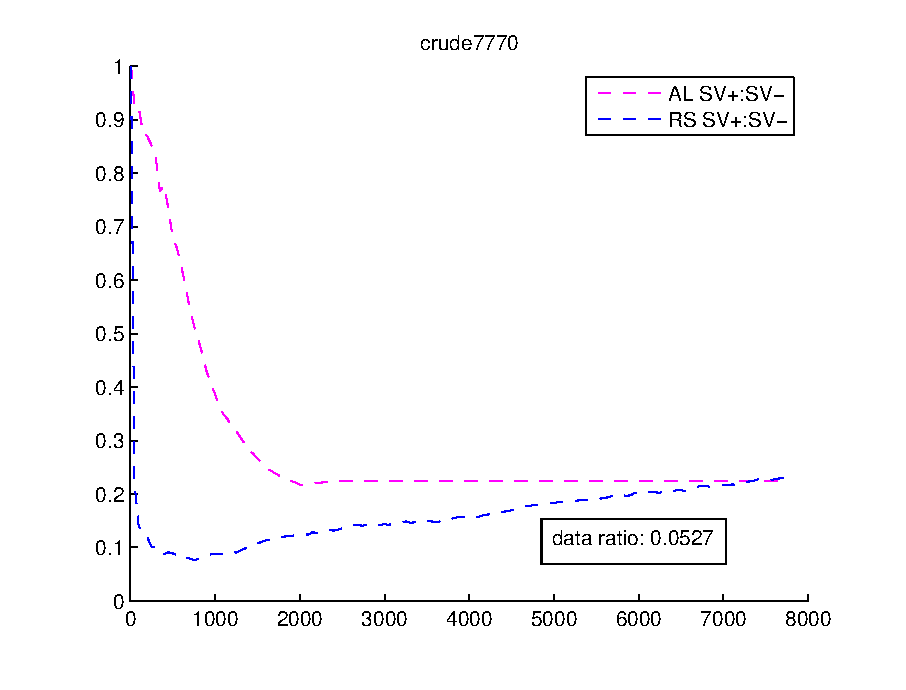
\includegraphics{Figures/lotb/cruderatio.eps}}
    \caption{Support Vector ratios in AL and RS}
    \label{cruderatio}
\end{figure}


We also compared the performance of early stopped AL with Batch algorithm. Table \ref{tbl:AUC} presents the g-means and the AUC values of the two methods. Data efficiency column for AL indicates that by processing only a portion of the examples from the training set, AL can achieve similar or even higher prediction performance than that of Batch which sees all the training examples. Another important observation from Table \ref{tbl:AUC} is that support vector imbalance ratios in the final models are much less than the class imbalance ratios of the datasets. This confirms our discussion of Figure \ref{fig:alimbshade}. The class imbalance ratio within the margins are much less than the class imbalance ratio of the entire data and active learning can be used to reach those informative examples which most likely become support vectors without seeing all the training examples.

In order to evaluate the methods at different thresholds, we also investigate the ROC curves as given in Figure \ref{fig:rocall}. The ROC curves of AL are similar and sometimes better than of the Batch algorithm (RS, seeing all the training examples). The AUC of AL and Batch are 0.8980 and 0.8910 respectively in the \emph{Adult} dataset. At the same number of training instances where AL is early stopped, AUC of RS can be substantially lower. As Figure \ref{fig:rocall} shows, the ROC curve of AL is markedly higher than that of RS (early stopping) and the AUC values are 0.8980 and 0.8725 respectively for \emph{Adult} dataset. These results suggest that AL converges faster than RS using fewer and informative instances and AL can get even higher prediction performance than the Batch algorithm by processing only a portion of the training set.

\begin{table*}[t!]\centering{
\caption{Comparison of g-means and AUC for AL and RS with entire training data (Batch).
Support vector ratios are given at the saturation point. Data efficiency corresponds to the percentage of training instances which AL processes to reach saturation.}
\begin{tabular}{l|l|r r|r r||r|r|c}
\hline
\multicolumn{2}{c|}{\multirow{2}{1cm}{Dataset}}
&\multicolumn{2}{c|}{g-means (\%)}
&\multicolumn{2}{c||}{AUC (\%)}
&Imb.&SV- /&\multirow{2}{12mm}{Data Efficiency}
\\
\cline{3-6}
\multicolumn{2}{c|}{}&Batch&AL&Batch&AL&Rat.&SV+\\
\hline\hline
\multirow{8}{1mm}{\begin{sideways}\parbox{12mm}{Reuters}\end{sideways}}
&Corn&85.55&86.59&99.95&99.95&41.9&3.13&11.6\%\\
&Crude&88.34&89.51&99.74&99.74&19.0&2.64&22.6\%\\
&Grain&91.56&91.56&99.91&99.91&16.9&3.08&29.6\%\\
&Interest&78.45&78.46&99.01&99.04&21.4&2.19&30.9\%\\
&Money-fx&81.43&82.79&98.69&98.71&13.4&2.19&18.7\%\\
&Ship&75.66&74.92&99.79&99.80&38.4&4.28&20.6\%\\
&Trade&82.52&82.52&99.23&99.26&20.1&2.22&15.4\%\\
&Wheat&89.54&89.55&99.64&99.69&35.7&3.38&11.6\%\\
\hline
\multirow{5}{1mm}{\begin{sideways}\parbox{12mm}{CiteSeer}\end{sideways}}
&AI&87.83&88.58&94.82&94.69&4.3&1.85&33.4\%\\
&COMM&93.02&93.65&98.13&98.18&4.2&2.47&21.3\%\\
&CRYPT&98.75&98.87&99.95&99.95&11.0&2.58&15.2\%\\
&DB&92.39&92.39&98.28&98.46&7.1&2.50&18.2\%\\
&OS&91.95&92.03&98.27&98.20&24.2&3.52&36.1\%\\
\hline
\multirow{3}{1mm}{\begin{sideways}\parbox{6mm}{UCI}\end{sideways}}
&Abalone-7&100.0&100.0&100.0&100.0&9.7&1.38&24.0\%\\
&Letter-A&99.28&99.54&99.99&99.99&24.4&1.46&27.8\%\\
&Satimage&82.41&83.30&95.13&95.75&9.7&2.62&41.7\%\\
\hline
\multicolumn{2}{c|}{USPS}&99.22&99.25&99.98&99.98&4.9&1.50&6.8\%\\
\hline
\multicolumn{2}{c|}{MNIST-8}&98.47&98.37&99.97&99.97&9.3&1.59&11.7\%\\
\hline
\end{tabular}
\label{tbl:AUC}

}
\end{table*}

In Figure \ref{cruderatio}, we investigate how the number of support vectors changes in AL and Random Sampling (RS). With random sampling, the instances are selected for the learner randomly from the entire pool of the training data. Therefore, the support vector imbalance ratio quickly approaches the data imbalance ratio. As learning continues, the learner should gradually see all the instances within the final margin and the support vector imbalance ratio decreases. At the end of training with RS, the support vector imbalance ratio is the data imbalance ratio within the margin. The support vector imbalance ratio curve of AL is drastically different than RS. AL intelligently picks the instances closest to the margin in each step. Since the data imbalance ratio within the margin is lower than data imbalance ratio, the support vectors in AL are more balanced than RS during learning. Using AL, the model saturates by seeing only 2000 (among 7770) training instances and reaches the final support vector imbalance ratio. Note that both methods achieve similar support vector imbalance ratios when learning finishes, but AL achieves this in the early steps of the learning.

We compare AL against several other strategies as well. Among them, undersampling (US), and an oversampling method (SMOTE) are examples of resampling techniques which require preprocessing. It has been shown that oversampling at random does not help to improve prediction performance \cite{Japkowicz_2002} therefore we use a more complex oversampling method, namely SMOTE.  Synthetic Minority Oversampling Technique (SMOTE) oversamples the minority class by creating synthetic examples rather than with replacement. The $k$ nearest positive neighbors of all positive instances are identified and synthetic positive examples are created and placed randomly along the line segments joining the $k$ minority class nearest neighbors.

\begin{table*}[t!]\centering{
\caption{Comparison of PRBEP and training time. }\small
\begin{tabular}{l|l|r r r r r|r r}
\hline
\multicolumn{2}{c|}{Metric}&\multicolumn{5}{c|}{PRBEP}&\multicolumn{2}{c}{Training time (sec.)}\\
\hline
\multicolumn{2}{c|}{Dataset}&Batch&US&SMOTE&DC&AL&SMOTE&AL\\
\hline
\hline
\multirow{8}{5mm}{\begin{sideways}\parbox{13mm}{Reuters}\end{sideways}}
&Corn&91.07&78.57&91.07&89.28&89.29&87&16\\
&Crude&87.83&85.70&87.83&87.83&87.83&129&41\\
&Grain&92.62&89.93&91.44&91.94&91.94&205&50\\
&Interest&76.33&74.04&77.86&75.57&75.57&116&42\\
&Money-fx&73.74&74.30&75.42&75.42&76.54&331&35\\
&Ship&86.52&86.50&88.76&89.89&89.89&49&32\\
&Trade&77.77&76.92&77.77&77.78&78.63&215&38\\
&Wheat&84.51&81.61&84.51&84.51&85.92&54&25\\
\hline
\multirow{5}{5mm}{\begin{sideways}\parbox{12mm}{CiteSeer}\end{sideways}}
&AI&78.80&80.68&78.99&78.79&79.17&1402&125\\
&COMM&86.59&86.76&86.59&86.59&86.77&1707&75\\
&CRYPT&97.89&97.47&97.89&97.89&97.89&310&19\\
&DB&86.36&86.61&86.98&86.36&86.36&526&41\\
&OS&84.07&83.19&84.07&84.07&84.07&93&23\\
\hline
\multirow{3}{5mm}{\begin{sideways}\parbox{6mm}{UCI}\end{sideways}}
&Abalone-7&100.0&100.0&100.0&100.0&100.0&16&4\\
&Letter-A&99.48&96.45&99.24&99.35&99.35&86&3\\
&Satimage&73.46&68.72&73.46&73.93&73.93&63&21\\
\hline
\multicolumn{2}{c|}{USPS}&98.44&98.44&98.13&98.44&98.75&4328&13\\
\hline
\multicolumn{2}{c|}{MNIST-8}&97.63&97.02&97.74&97.63&97.74&83,339&1,048\\
\hline

\end{tabular}
\label{tbl:results}
}
\end{table*}

As an algorithmic method to compare, we use the method of assigning different costs (DC) to the positive and negative classes as the misclassification penalty parameter. For instance, if the imbalance ratio of the data is 19:1 in favor of the negative class, the cost of misclassifying a positive instance is set to be 19 times greater than that of misclassifying a negative one. We use the online SVM package LASVM\footnote{Available at http://leon.bottou.org/projects/lasvm} in all experiments. Other than the results of the methods addressing class imbalance problem, we also give results of Batch algorithm with the original training set to form a baseline. LASVM is run in random sampling mode for US, SMOTE and DC.

We present the comparisons of the methods for g-means performance metric for several datasets in Figure \ref{eightgraphs}. The right border of the shaded pink area is the place where the aforementioned early stopping strategy is applied.  The curves in the graphs are averages of 10 runs. For completeness, we did not stop the AL experiments at the early stopping point but allow them to run on the entire training set. Table \ref{tbl:results} presents the PRBEP of the methods and the total running times of the SMOTE and AL on 18 benchmark and real-world datasets. The results for active learning in Table \ref{tbl:results} depict the results in the early stopping points. The results for the other methods in Table \ref{tbl:results} depict the values at the end of the curves --when trained with the entire dataset-- since those methods do not employ any early stopping criteria. We did not apply early stopping criteria to the other methods because as observed from Figure \ref{eightgraphs}, no early stopping criteria would achieve a comparable training time with of AL's training time without a significant loss in their prediction performance based on convergence time. The other methods converge to similar levels of g-means when nearly all training instances are used, and applying an early stopping criteria would have little, if any, effect on their training times.

\begin{figure*}[t]
    \hspace{-5mm}
        \scalebox{0.51}{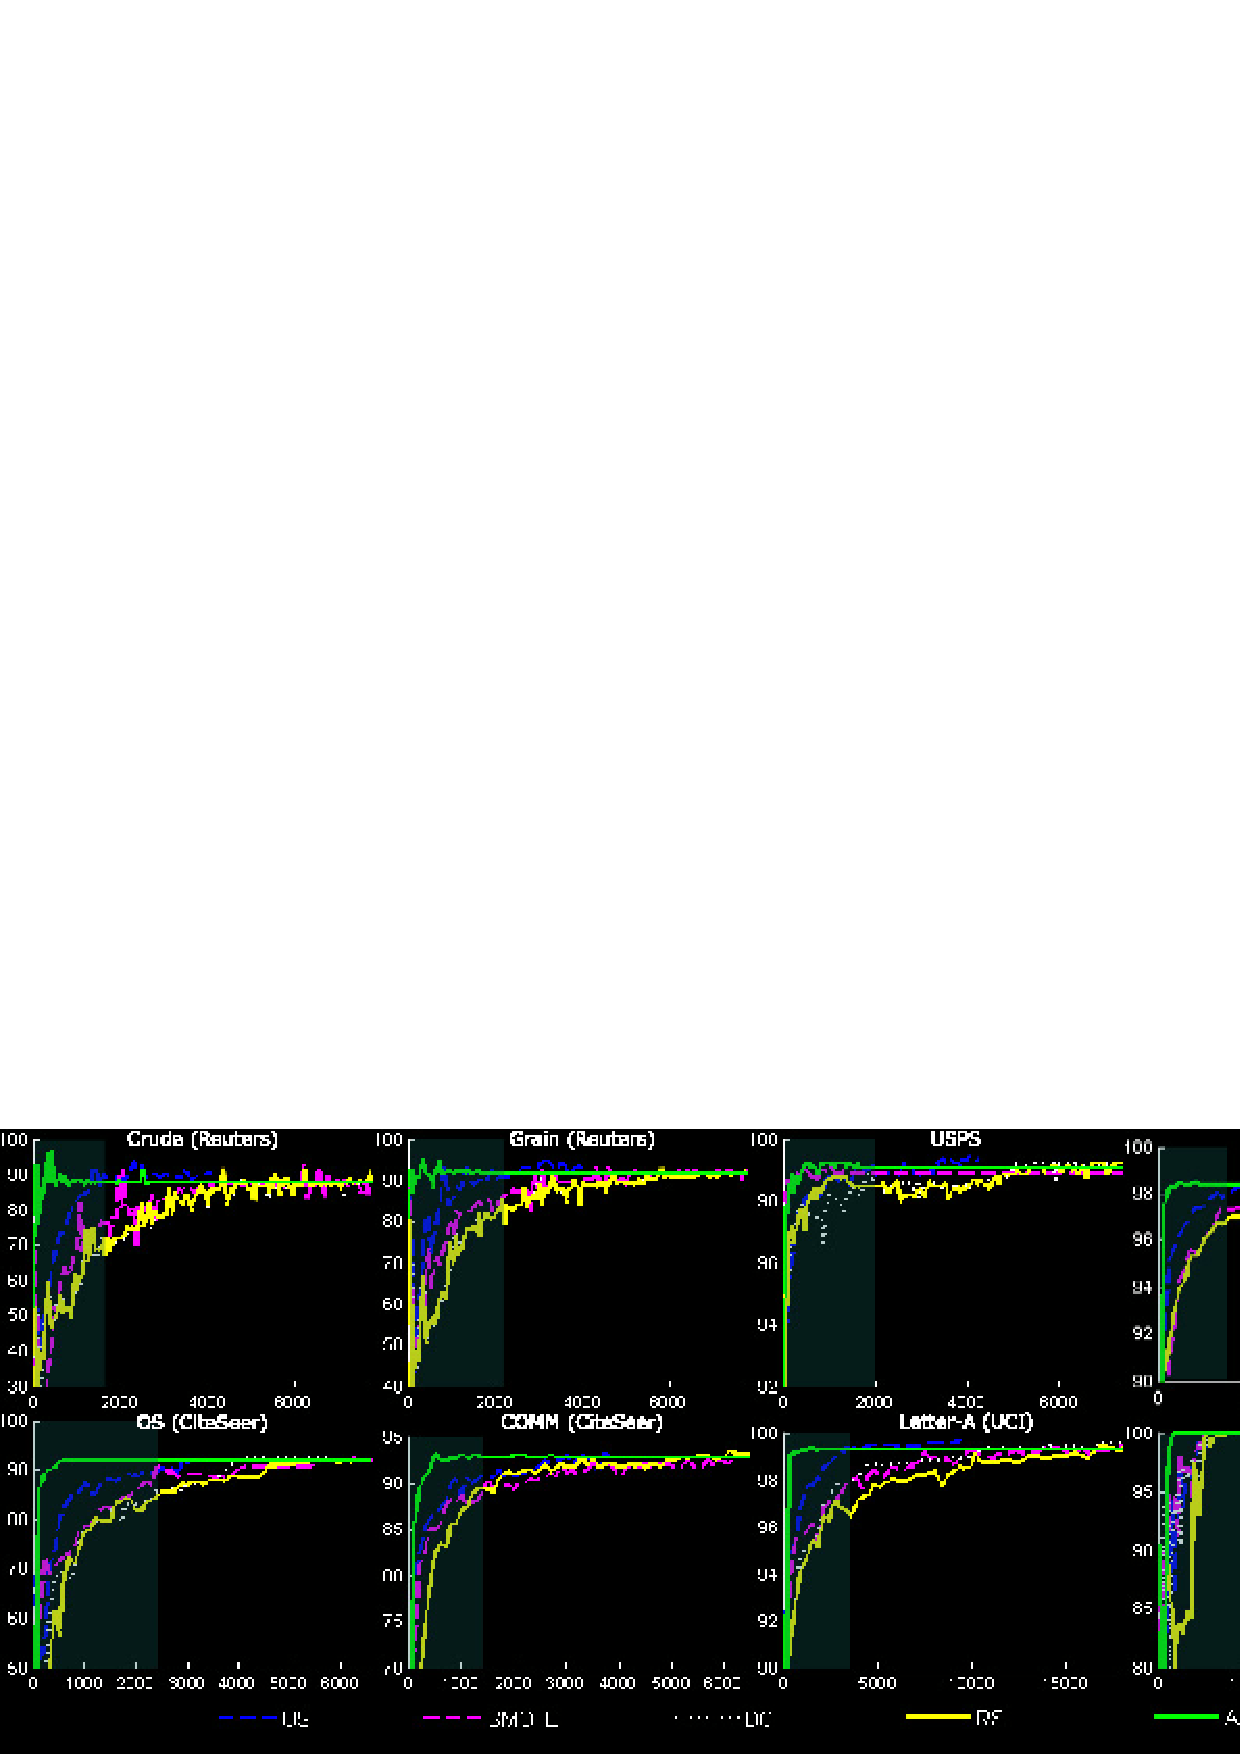
\includegraphics{Figures/lotb/big8.pdf}}
    \caption{Comparisons of g-means. The right border of the shaded area corresponds to the early stopping point.}
    \label{eightgraphs}
\end{figure*}

\begin{table}[!t]\centering \small{
\caption{Comparison of ranks of different methods in PRBEP. The values in bold correspond to the cases where AL win. AL wins in 12 out of 18 cases in PRBEP.}
\begin{tabular}{l|l|c c c c c}
\hline
\multicolumn{2}{c|}{Metric}&\multicolumn{5}{c}{Rank}\\\hline
\multicolumn{2}{c|}{Dataset}&Batch&US&SMOTE&DC&AL\\
\hline\hline
\multirow{5}{5mm}{\begin{sideways}\parbox{13mm}{Reuters}\end{sideways}}
&Corn&1&5&1&4&3\\
&Crude&1&5&1&1&\textbf{1}\\
&Grain&1&5&4&2&2\\
&Interest&2&5&1&3&3\\
&Money-fx&5&4&2&2&\textbf{1}\\
&Ship&4&5&3&1&\textbf{1}\\
&Trade&3&5&3&2&\textbf{1}\\
&Wheat&2&5&2&2&\textbf{1}\\
\hline
\multirow{5}{5mm}{\begin{sideways}\parbox{12mm}{CiteSeer}\end{sideways}}
&AI&4&1&3&5&2\\
&COMM&3&2&3&3&\textbf{1}\\
&CRYPT&1&5&1&1&\textbf{1}\\
&DB&3&2&1&3&3\\
&OS&1&5&1&1&\textbf{1}\\
\hline
\multirow{2}{5mm}{\begin{sideways}\parbox{6mm}{UCI}\end{sideways}}
&Abalone-7&1&1&1&1&\textbf{1}\\
&Letter-A&1&5&4&2&2\\
&Satimage&3&5&3&1&\textbf{1}\\
\hline
\multicolumn{2}{c|}{USPS}&2&2&5&2&\textbf{1}\\
\hline
\multicolumn{2}{c|}{MNIST-8}&3&5&1&3&\textbf{1}\\
\hline
\hline
\multicolumn{2}{c|}{Avg. Rank }&2.28&4.00&2.22&2.17&\textbf{1.50}\\
\hline
\end{tabular}
\label{tbl:rankresults}
}
\end{table}

Since AL involves discarding some instances from the training set, it can be perceived as a type of undersampling method. Unlike US which discards majority samples randomly, AL performs an intelligent search for the most informative ones adaptively in each iteration according to the current hyperplane. In datasets where class imbalance ratio is high such as \emph{corn}, \emph{wheat}, \emph{letter} and \emph{satimage}, we observe significant decrease in PRBEP of US (see Table 3). Note that US's undersampling rate for the majority class in each category is set to the same value as the final support vector ratio which AL reaches in the early stopping point and RS reaches when it sees the entire training data. Although the class imbalance ratio provided to the learner in AL and US are the same, AL achieves significantly better PRBEP performance metric than US. The Wilcoxon signed-rank test (2-tailed) reveals that the zero median hypothesis can be rejected at the significance level 1\% (p=0.0015), implying that AL performs statistically better than US in these 18 datasets. These results reveal the importance of using the informative instances for learning.

Table \ref{tbl:rankresults} presents the rank of PRBEP prediction performance of the five approaches in a variety of datasets. The values in bold correspond to the cases where AL wins and it's clear that winning cases are very frequent for AL (12 out of 18 cases). The average rank also indicates that AL achieves the best PRBEP among the five methods. SMOTE and DC achieve higher PRBEP than the Batch algorithm. The loss of information when undersampling the majority class affects US's prediction performance. Table \ref{tbl:results} also gives the comparison of the computation times of the AL and SMOTE. Note that SMOTE requires significantly long preprocessing time which dominates the training time in large datasets, e.g., MNIST-8 dataset. The low computation cost, scalability and high prediction performance of AL suggest that AL can efficiently handle the class imbalance problem.


%%%%%%%%%%%%%%%%%%%%%%%%
%%%%%%%%%%%%%%%%%%%%%%%%
%%%%%%%%%%%%%%%%%%%%%%%%
%%%%%%%%%%%%%%%%%%%%%%%%
%%%         V     I     R     T     U     A     L          %%%
%%%%%%%%%%%%%%%%%%%%%%%%
%%%%%%%%%%%%%%%%%%%%%%%%
%%%%%%%%%%%%%%%%%%%%%%%%
%%%%%%%%%%%%%%%%%%%%%%%%
%%%%%%%%%%%%%%%%%%%%%%%%


\section{Adaptive Resampling with Active Learning for Imbalanced Data Classification}
\label{virtual}
In Section \ref{lotb_experiments}, our analysis shows the effectiveness of active learning in imbalanced datasets under various data and learner characteristics. One comparison highlighted the benefits over oversampling techniques, and in this section, we present a methodology for using active learning as an oversampling strategy for imbalanced data classification.

In supervised learning, a common strategy to overcome the rarity problem is to resample the original dataset to decrease the overall level of class imbalance. Resampling is done either by oversampling the minority (positive) class and/or undersampling the majority (negative) class until the classes are approximately equally represented \cite{Chawla_2002,Japkowicz_2000,Kubat_1997,Ling_1998}. Oversampling, in its simplest form, achieves a more balanced class distribution either by duplicating minority class instances, or introducing new synthetic instances that belong to the minority class \cite{Chawla_2002}. No information is lost in oversampling since all original instances of the minority and the majority classes are retained in the oversampled dataset. The other strategy to reduce the class imbalance is undersampling, which eliminates some majority class instances mostly by random sampling.

Even though both approaches address the class imbalance problem, they also suffer some drawbacks. The undersampling strategy can potentially sacrifice the prediction performance of the learner, since it is possible to discard informative instances that the learner might benefit. The oversampling strategy, on the other hand, can be overwhelming in case of very large training data. If a complex oversampling method is used, it suffers from high computational costs during preprocessing of the data. Worse yet, oversampling causes longer training time during the learning process due to the increased number of training instances. In addition to suffering from worse runtime performance, it is also inefficient in terms of memory requirements since more instances in addition to the original training data have to be stored. Other costs associated with the learning process (i.e., extended kernel matrix in kernel classification algorithms) are other drawbacks of oversampling.

\subsection{Virtual Instance Resampling Technique Using Active Learning}
In this section, we focus on the oversampling strategy for imbalanced data classification and investigate how it can benefit from the principles of active learning. Our goal is to remedy the efficiency drawbacks of oversampling in imbalanced data classification and use an active learning strategy to generate minority class instances only if they can be useful to the learner. \textsc{Virtual} (Virtual Instance Resampling Technique Using Active Learning)~\cite{Ertekin_dissertation} is a hybrid method of oversampling and active learning that forms an adaptive technique for resampling of the minority class instances. In contrast to traditional oversampling techniques that act as an \textit{offline} step that generate virtual instances of the minority class prior to the training process, \textsc{Virtual} leverages the power of active learning to intelligently and adaptively oversample the data \textit{during} training, removing the need for an offline and separate preprocessing stage. Similar to the discussions in the previous section, \textsc{Virtual} also employs an online SVM-based active learning strategy. In this setting, the informativeness of instances are measured by their distance to their hyperplane, and the most informative instances are selected as the support vectors. \textsc{Virtual} targets the set of support vectors during training, and resamples new instances based on this set. Since most support vectors are found during early stages of training, corresponding virtual examples are also created in the early stages. This prevents the algorithm from creating excessive and redundant virtual instances and integrating the resampling process into the training stage improves the efficiency and generalization performance of the learner compared to other competitive oversampling techniques.

We first briefly discuss the active learning step of the \textsc{Virtual} and explain the virtual instance generation process of the algorithm. We then highlight the advantages of the proposed method.

\subsubsection{Active Selection of Instances}
Let $S$ denote the pool of real and virtual training examples unseen by the learner at each active learning step. Instead of searching for the most informative instance among all the samples in $S$, \textsc{Virtual} queries a randomly picked smaller pool from $S$ based on the ``59 trick'' that we discussed in section \ref{ALpools}. From the small pool, \textsc{Virtual} selects an instance that is closest to the hyperplane according to the current model. If the selected instance is a real positive instance (from the original training data) and becomes a support vector, \textsc{Virtual} advances to the oversampling step, which we explain in the following section. Otherwise, the algorithm proceeds to the next iteration to select another instance.


\begin{algo}[!b]
\begin{center} \small
\begin{tabular}{l}
{\bfseries Define:} \\
~~$X=\{x_1, x_2, \cdots, x_n\}$ : training instances \\
~~$X^+_{R}$ : positive real training instances\\
~~$S$ : pool of training instances for SVM\\
~~$v$ : \# virtual instances to create in each iteration\\
~~$L$ : size of the small set of randomly picked samples\\
~~~~~~~ for active sample selection\\
\hline
\\
1.~~Initialize $S \leftarrow X$\\
2.~~{\bfseries while} $S \neq \emptyset$\\
3.~~~~~~//~\textit{Active sample selection step}\\
4.~~~~~~$d_{min}\leftarrow \infty$\\
5.~~~~~~{\bfseries for} $i \leftarrow 1$ to $L$\\
6.~~~~~~~~~~$x_j \leftarrow RandomSelect(S)$\\
7.~~~~~~~~~~{\bfseries If} $d(x_j, hyperplane) < d_{min}$\\
8.~~~~~~~~~~~~~~$d_{min}\leftarrow d(x_j, hyperplane)$\\
9.~~~~~~~~~~~~~~$candidate \leftarrow x_j$\\
10.~~~~~~~~~{\bfseries end}\\
11.~~~~~{\bfseries end}\\
12.~~~~~$x_s \leftarrow candidate$\\
13.~~~~~//~\textit{Virtual Instance Generation}\\
14.~~~~~{\bfseries If} $x_s$ becomes SV {\bfseries and} $x_s \in X^+_{R}$\\
15.~~~~~~~~~$K \leftarrow$ $k$ nearest neighbors of $x_s$\\
16.~~~~~~~~~{\bfseries for} $i \leftarrow 1$ to $v$\\
17.~~~~~~~~~~~~~$x_m \leftarrow RandomSelect(K)$\\
18.~~~~~~~~~~~~~//~Create a virtual positive instance $x^v_{s,m}$ between $x_s$ and $x_m$ \\
19.~~~~~~~~~~~~~$\lambda$=random number between 0 and 1\\
20.~~~~~~~~~~~~~$x^v_{s,m} = \lambda \cdot x_s + (1-\lambda)x_m$\\
21.~~~~~~~~~~~~~$S \leftarrow S \cup x^v_{s,m}$\\
22.~~~~~~~~~{\bfseries end}\\
23.~~~~~{\bfseries end}\\
24.~~~~~$S \leftarrow S - x_s$\\
25.~{\bfseries end}
\vspace{-3mm}
\end{tabular}
\end{center}
\caption{VIRTUAL}
\label{algo_virtual}
\end{algo}

\subsubsection{Virtual Instance Generation}
\textsc{Virtual} oversamples the real minority class instance (from the original training data) which become a support vector in the current iteration. It selects the $k$ nearest minority class neighbors $(x_{i\rightarrow 1} \cdots x_{i \rightarrow k})$ of $x_i$ based on their similarities in the kernel transformed higher dimensional feature space. We limit the neighboring instances of $x_i$ to the minority class so that the new virtual instances lie within the minority class distribution. Depending on the amount of over-sampling required, the algorithm creates $v$ virtual instances. Each virtual instance lies on any of the line segments joining $x_i$ and its neighbor $x_{i\rightarrow j}\ (j=1,...,k)$. In other words, a neighbor $x_{i \rightarrow j}$ is randomly picked and the virtual instance is created as $\bar{x}_v = \lambda \cdot x_i + (1-\lambda)x_{i \rightarrow j}$,  where $\lambda\in(0,1)$ determines the placement of $\bar{x}_v$ between $x_i$ and $x_{i \rightarrow j}$. All $v$ virtual instances are added to $S$ and are eligible to be picked by the active learner in the subsequent iterations.

The pseudocode of \textsc{Virtual} given in Algorithm \ref{algo_virtual}  depicts the two processes described above. In the beginning, the pool $S$ contains all real instances in the training set. At the end of each iteration, the instance selected is removed from $S$, and any virtual instances generated are included in the pool $S$. In this pseudocode, \textsc{Virtual} terminates when there are no instances in $S$. In Section \ref{early_stop}, we propose an early stopping criteria for \textsc{Virtual}.

\begin{figure*}[t!bp]
  \begin{center}
     \mbox{
      \subfigure[Oversampling with SMOTE]{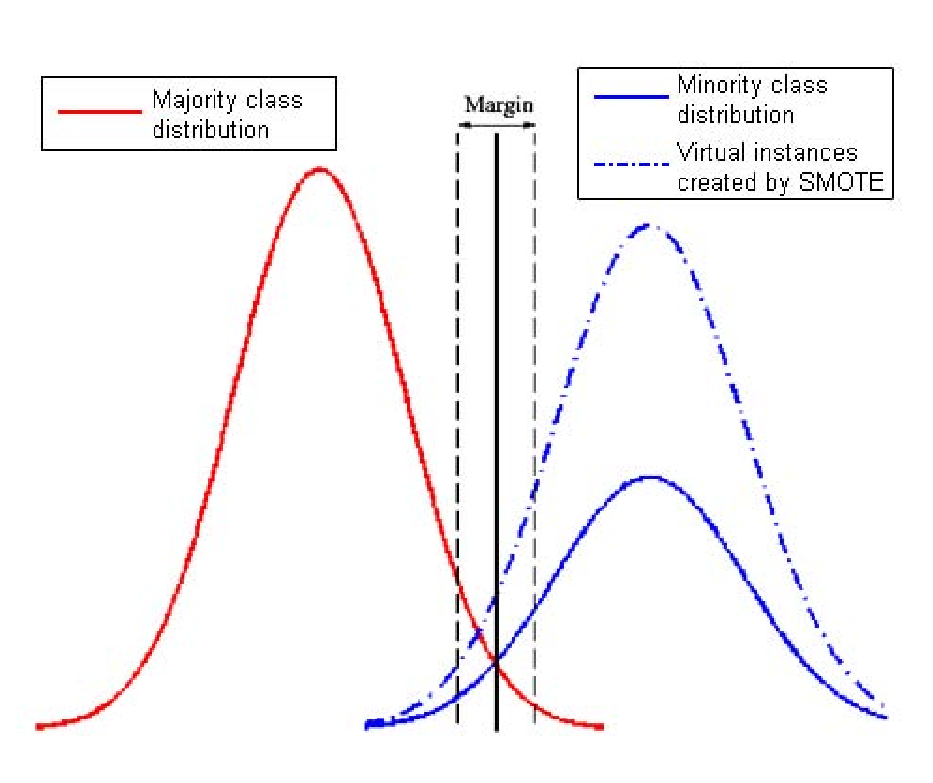
\includegraphics[width=0.45\textwidth, height=4.2cm]{Figures/virtual/smote_proc.eps}
      \label{fig:smote_sample}
      } \quad
      \subfigure[Oversampling with \textsc{Virtual}]{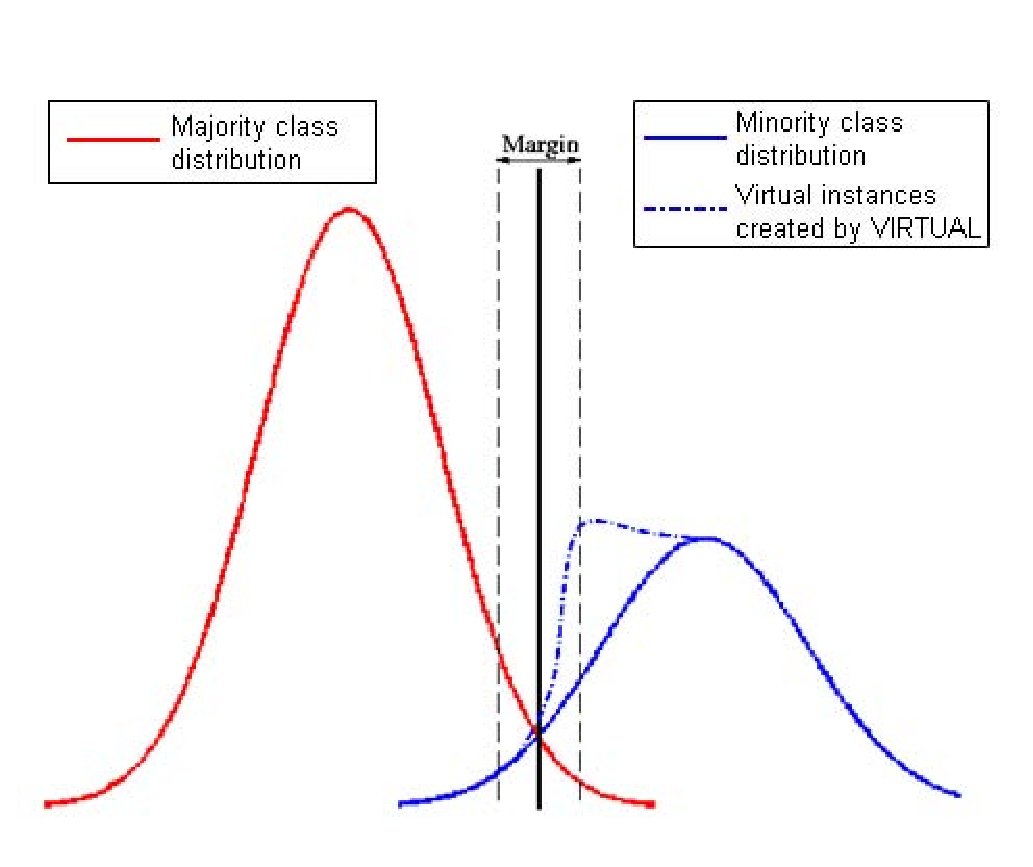
\includegraphics[width=0.45\textwidth, height=4.2cm]{Figures/virtual/virtual_proc.eps}
      \label{fig:virtual_sample}
      }
      }
    \caption{Comparison of oversampling the minority class with SMOTE and VIRTUAL. }
    \label{fig:oversample}
  \end{center}
\end{figure*}

\subsection{Remarks on VIRTUAL}
We compare \textsc{Virtual} with a popular oversampling technique SMOTE to  illustrate the advantages of the proposed algorithm. Figure \ref{fig:oversample} shows the different behavior of how SMOTE and \textsc{Virtual} create virtual instances for the minority class. SMOTE creates virtual instance(s) for each positive example (see Figure \ref{fig:smote_sample}), whereas \textsc{Virtual} creates the majority of virtual instances around the positive canonical hyperplane (shown with a dashed line in Figure \ref{fig:virtual_sample}). Note that a large portion of virtual instances created by SMOTE are far away from the hyperplane and thus are not likely to be selected as support vectors. \textsc{Virtual}, on the other hand, generates virtual instances near the real positive support vectors adaptively in the learning process. Hence the virtual instances are near the hyperplane and thus are more informative.

We further analyze the computation complexity of SMOTE and \textsc{Virtual}.  The computation complexity of \textsc{Virtual} is $O(\left|SV(+) \right|\cdot v \cdot \mathcal{C})$, where $v$ is the number of virtual instances created for a real positive support vector in each iteration, $\left|SV(+) \right|$ is the number of positive support vectors and $\mathcal{C}$ is the cost of finding k nearest neighbors. The computation complexity of SMOTE is $O(\left| X_R^+\right| \cdot v \cdot \mathcal{C})$, where $\left| X_R^+\right|$ is the number of positive training instances. $\mathcal{C}$ depends on the approach for finding k nearest neighbors. The naive implementation searches all $N$ training instances for the nearest neighbors and thus $\mathcal{C}=kN$. Using advanced data structure such as kd-tree, $\mathcal{C}=k\log N$. Since $\left|SV(+) \right|$ is typically much less than $\left| X_R^+\right|$, \textsc{Virtual} incurs lower computation overhead than SMOTE. Also, with fewer virtual instances created, the learner is less burdened with \textsc{Virtual}. We demonstrate with empirical results that the virtual instances created with \textsc{Virtual} are more informative and the prediction performance is also improved.

\subsection{Experiments}
We conduct a series of experiments both on synthetic and real-world datasets to demonstrate the efficacy of \textsc{Virtual}. We compare \textsc{Virtual} with two systems, Active Learning (AL) and SMOTE. AL solely adopts the traditional active learning strategy without preprocessing or creating any virtual instances during learning. SMOTE, on the other hand, preprocesses the data by creating virtual instances before training and uses random sampling in learning. Experiments elicit the advantages of adaptive virtual sample creation in \textsc{Virtual}.

\begin{figure}[b!]
\begin{center}
\hspace{-10mm}
\subfigure {
\includegraphics[width=40mm]{Figures/virtual/wf_imb_rt_1.jpg}
}
\subfigure {
\includegraphics[width=40mm]{Figures/virtual/wf_imb_rt_2.jpg}
}
\subfigure {
\includegraphics[width=40mm]{Figures/virtual/wf_imb_rt_3.jpg}
} \\
\hspace{-10mm}
\subfigure {
\includegraphics[width=40mm]{Figures/virtual/wf_imb_rt_4.jpg}
}
\subfigure {
\includegraphics[width=40mm]{Figures/virtual/wf_imb_rt_5.jpg}
}
\subfigure {
\includegraphics[width=40mm]{Figures/virtual/wf_imb_rt_legend.jpg}
}
\end{center}
  \caption{Comparison of Active Learning and VIRTUAL on the \emph{Waveform} dataset with
  different imbalance ratios (Imb.R.=2, 4, 8, 16, 32). The test results are average of ten runs.}
  \label{fig:waveform}
\end{figure}


\subsubsection{Simulation Study}\label{early_stop}
The popular waveform example is widely used in classification literature \cite{Breiman84}. In this example, three shifted triangular waveforms
\begin{eqnarray*}
v_1(j)&=&max(6-|j-11|,0)\\
v_2(j)&=&v_1(j-4)\\
v_3(j)&=&v_1(j+4)
\end{eqnarray*}
are linearly combined into 21 variables:
\[
x_j  = \left\{ \begin{array}{l}
 u \cdot v_1 (j) + (1 - u)v_2 (j) + \varepsilon _j,\ \mbox{Class 1}  \\
 u \cdot v_1 (j) + (1 - u)v_3 (j) + \varepsilon _j,\ \mbox{Class 2}  \\
 u \cdot v_2 (j) + (1 - u)v_3 (j) + \varepsilon _j,\ \mbox{Class 3} \\
 \end{array} \right.
\]
where $ j=1,2,...,21$, $u$ is uniformly distributed on $(0,1)$ and $\varepsilon _j$ is the normal Gaussian noise. In our case, we use samples from Class 1 as positive samples and the others as negative and thus the imbalance ratio is 2. We randomly draw 4,000 samples for training and independently draw 1,000 samples for testing.

To showcase the different behavior of AL and \textsc{Virtual} in different imbalance ratio (Imb.R.) data, we undersample the positive class to obtain five datasets (\emph{Waveform} Imb.R.= $2^1, 2^2, 2^3, 2^4, 2^5$). Figure \ref{fig:waveform} demonstrates the g-means of AL and \textsc{Virtual} in these five datasets. We observe that when data is moderately imbalanced (Imb.R.=2, 4), the g-means curves of the two methods are close to each other. When the imbalance ratio increases, the g-means of AL drops faster than that of \textsc{Virtual} and thus the gap widens. In the \emph{Waveform} Imb.R. 32 dataset, there are 83 positive instances and AL uses them all as support vectors. Since \textsc{Virtual} (v=1) creates a virtual instance for each real positive support vector, it creates 83 positive virtual instances and most of them are selected as support vectors (see Figure \ref{fig:waveform-sv}). As a result, the number of positive support vectors nearly doubles and the number of positive and negative support vectors is more balanced. Figure \ref{fig:waveform} compares the g-means of AL and \textsc{Virtual} for different class imbalance ratios and illustrates that these adaptively created positive training instances in \textsc{Virtual} contribute to the improvement in g-means over AL. Therefore, \textsc{Virtual} is shown to be more resilient to imbalanced data.

\begin{figure*}[t!]
  \begin{center}
     \mbox{
      \subfigure[Number of support vectors in VIRTUAL versus number of training instances in \emph{Waveform} (Imb.R.=32)]{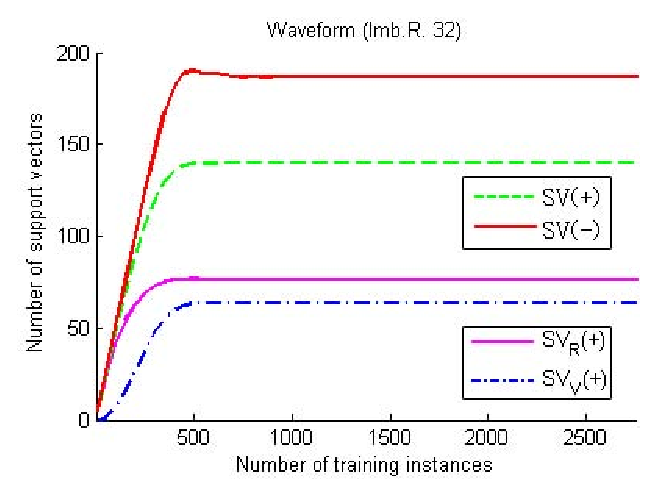
\includegraphics[width=0.47\textwidth, height=3.9cm]{Figures/virtual/wf-32sv-proc.eps}
      \label{fig:waveform-sv}
      } \quad
      \subfigure[Saturation of number of support vectors and g-means for \emph{Waveform} (Imb.R.=4). The vertical line indicates where support vectors saturate and training stops.]{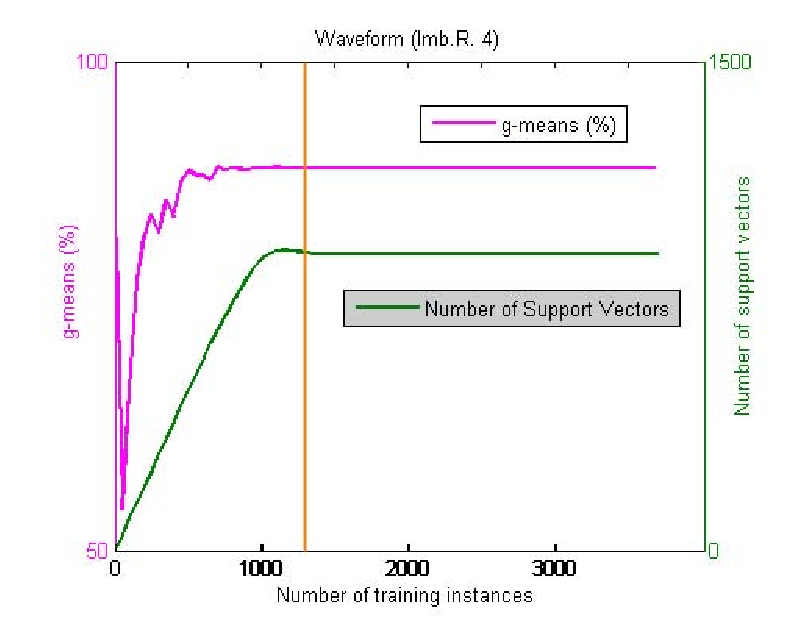
\includegraphics[width=0.47\textwidth, height=3.9cm]{Figures/virtual/wf4-sv.eps}
      \label{fig:waveform-sv-gmeans}
      }
      }
    \caption{Growth of the number of support vectors for \emph{Waveform}}
    \label{fig:waveform-sv-all}
  \end{center}
\end{figure*}

Figure \ref{fig:waveform-sv} further unpacks the adaptive learning process of \textsc{Virtual} in the \emph{Waveform} Imb.R. 32 dataset. When the first 150 training instances are seen, the number of real positive support vectors ($SV_R(+)$) and negative support vectors ($SV(-)$) is balanced. This effect is due to the active learning strategy, because in early iterations active learning picks positive and negative samples in a balanced manner whereas random sampling selects examples proportional to the data imbalance ratio. In this stage, the number of virtual positive instances is relatively small
compared to the real positive instances and thus few are selected into the model. Later, the real positive samples are selected more slowly (deviating from the straight line) and they are eventually exhausted. During this stage, virtual positive instances continue to be created and a large portion of them are selected into the model. Finally, the model becomes saturated using only 500 of the original total 2,757 training instances. By creating virtual examples, \textsc{Virtual} nearly doubles the number of positive support vectors and thus the support vector ratio becomes more balanced. As seen in Figure \ref{fig:waveform}, the adaptively created virtual examples help to guide the learner to achieve better g-means. This experiments on artificial dataset demonstrates the superiority of \textsc{Virtual} over AL in more imbalanced datasets.

In Figure \ref{fig:waveform-sv-gmeans}, we observe that when the number of support vectors saturates g-means also stabilizes. Seeing additional instances after a point does not change the model, as the
training instances in the margin are exhausted. Accordingly, we apply an early stopping criteria to eliminate the learning stage which has little, if any, impact on the prediction performance. A theoretically sound method to stop training is to check if there are still unseen training instances in the margin, the distance of the newly selected instance is compared to the support vectors of the current model. If the new selected instance by active learning (closest to the hyperplane) is not closer than any of the support vectors, we conclude that the margin is exhausted. A practical implementation of this idea is to count the number of support vectors during the active learning process.  If the number of the support vectors stabilizes, it implies that all possible support vectors have been selected into the model. Early stopping shortens the training time without sacrificing prediction performance. We adopt this strategy in our experiments to find the early stopping points where active learning is used.

\begin{table}[ht] \small
\caption{The Reuters and 4 UCI datasets.} \centering
\begin{tabular}{l|l|c@{\hspace{2mm}}r@{\hspace{2mm}}r@{\hspace{2mm}}c}
\hline
\multicolumn{2}{c|}{Dataset}&\#Feature&\#Pos&\#Neg&Imb. Ratio\\
\hline\hline
\multirow{10}{2mm}{\begin{sideways}\parbox{13mm}{Reuters}\end{sideways}}
&acq&8315&1650&6120&3.7\\
&corn&8315&181&7589&41.9\\
&crude&8315&389&7381&19.0\\
&earn&8315&2877&4893&1.7\\
&grain&8315&433&7337&16.9\\
&interest& 8315 &347&7423&21.4\\
&money-fx& 8315 &538&7232&13.4\\
&ship& 8315 &197&7573&38.4\\
&trade&8315&369&7401&20.1\\
&wheat& 8315 &212&7558&35.7\\
\hline\hline
\multirow{4}{2mm}{\begin{sideways}\parbox{5mm}{UCI}\end{sideways}}
&abalone&9&352&3407&9.7\\
&breast&9&172&320&1.9\\
&letter&16&710&17290&24.4\\
&satimage&36&415&4020&9.7\\
\hline
\end{tabular}
\label{tbl:virtual_datasets}
\end{table}

\subsubsection{Experiments on Real-World Data}
We study the performance of the algorithm on real-world data using several benchmark datasets. On the \emph{Reuters-21578} dataset, we test the algorithms with the top 10 most populated categories. In each category relevant instances are labeled as positive and the remaining as negative. We also used 4 benchmark datasets from the popular UCI Machine Learning Repository. \emph{Letter} and \emph{satimage} are image datasets. The `letter A' is used as the positive class in \emph{letter} and `class 4' (damp grey soil) is used as positive class in \emph{satimage}. \emph{Abalone} and \emph{Wisconsin breast cancer} (\emph{breast}) are biology and medical diagnosis datasets respectively. In \emph{abalone}, instances labeled as `class 7' form the positive class and instances labeled as `m.o.ant' constitute the positive class in \emph{breast}. These datasets cover a wide range of data imbalance ratio (see Table \ref{tbl:virtual_datasets}).

\begin{figure*}[!b]
  \centering
  \scalebox{1}
  {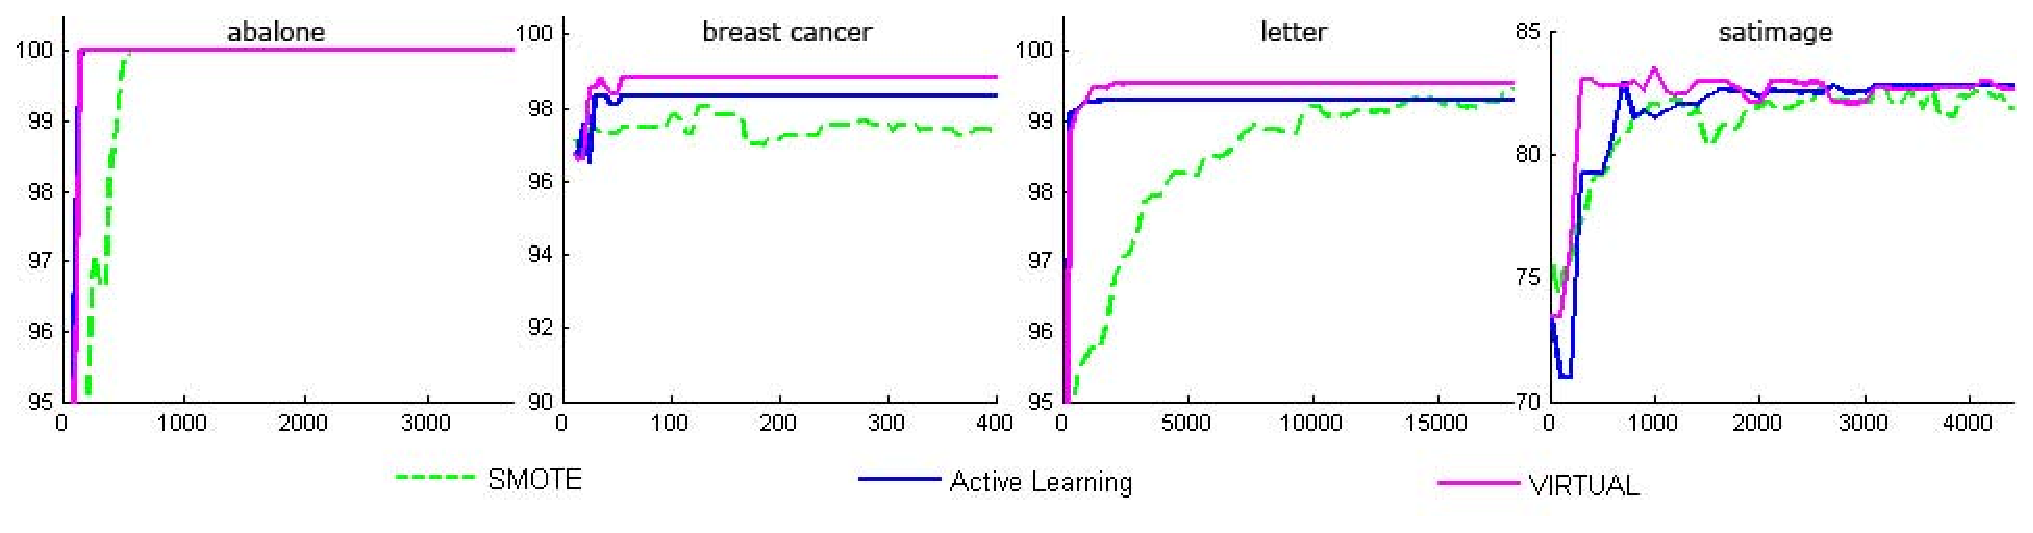
\includegraphics[width=\textwidth]{Figures/virtual/uci-graphs.eps}}\\
  \caption{Comparison of SMOTE, AL and VIRTUAL on \emph{UCI} datasets.
  We present the g-means (\%) (y-axis) of the current model for the test set
  vs. the number of training samples (x-axis) seen.}
  \label{fig:uci}
\end{figure*}

\begin{figure*}[!b]
  \centering
  \scalebox{1}
  {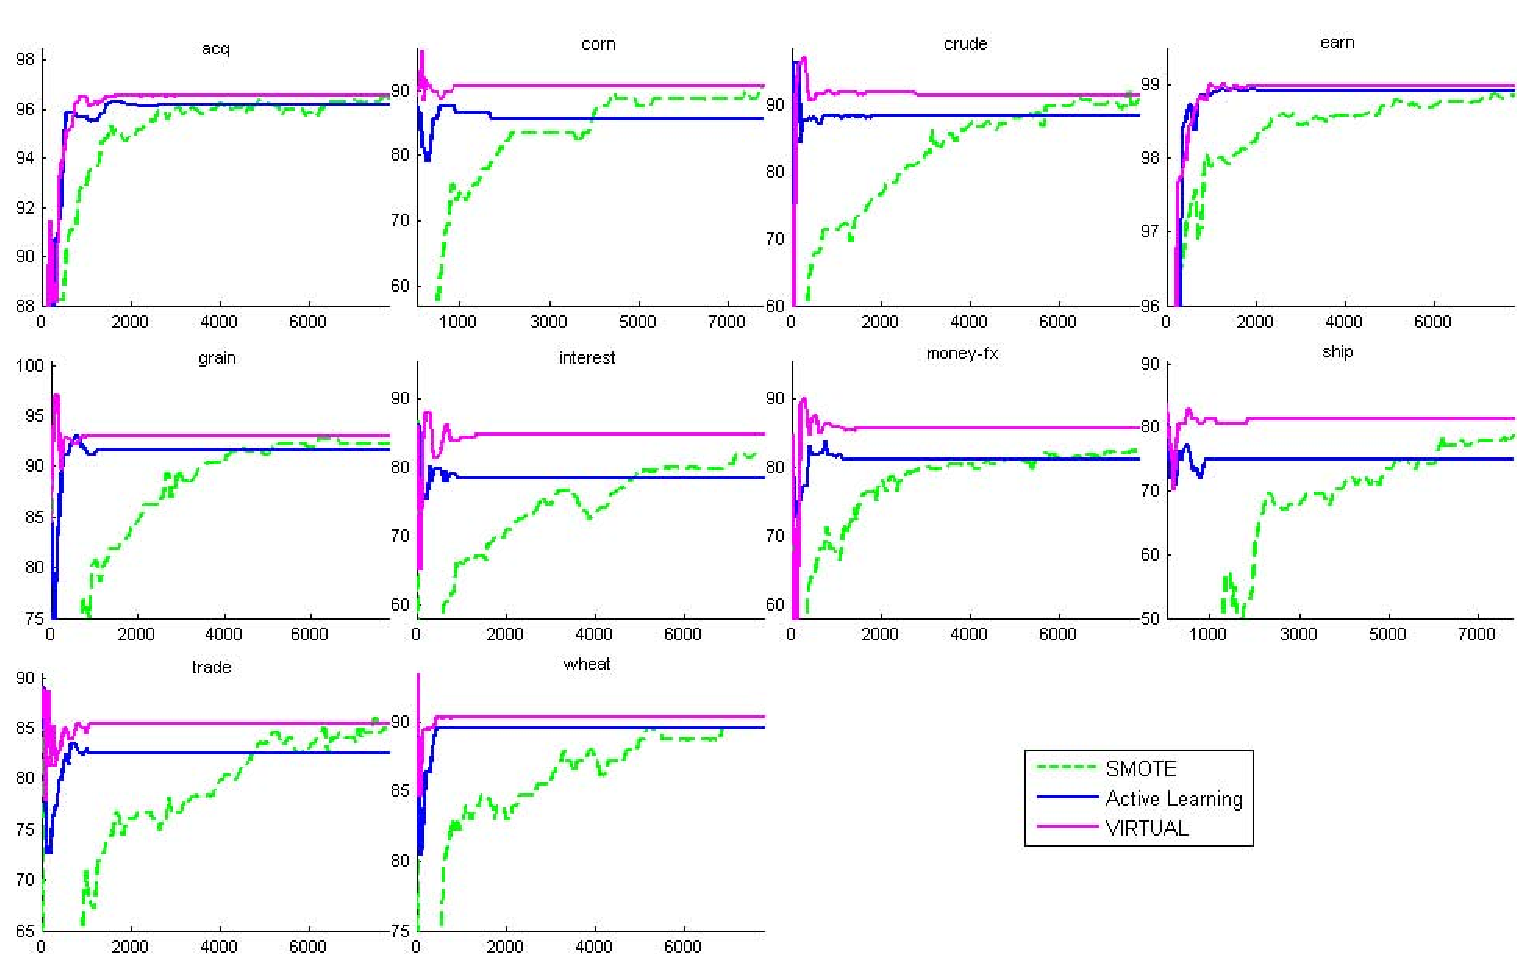
\includegraphics[width=\textwidth]{Figures/virtual/reuters.eps}}\\
  \caption{Comparison of SMOTE, AL and VIRTUAL on 10 largest categories of \emph{Reuters-21578}.
  We show the g-means (\%) (y-axis) of the current model for the test set
  versus the number of training samples (x-axis) seen.}
  \label{fig:reuters}
\end{figure*}

In Figures \ref{fig:uci} and \ref{fig:reuters},  we provide the details on the behavior of the three algorithms, SMOTE, AL and \textsc{Virtual}. For the Reuters datasets (Figure \ref{fig:reuters}), we note that in all the 10 categories \textsc{Virtual} outperforms AL in g-means metric after saturation. The difference in performance is most pronounced in the more imbalanced categories, e.g. \emph{corn}, \emph{interest} and \emph{ship}. In the less imbalanced datasets such as \emph{acq} and \emph{earn}, the difference in g-means of both methods is less noticeable. The g-means of SMOTE converges much slower than both AL and \textsc{Virtual}. However, SMOTE converges to higher g-means than AL in some of the categories, indicating that the virtual positive examples provide additional information that can be used to improve the model. \textsc{Virtual} converges to the same or even higher g-means than SMOTE while generating fewer virtual instances. For the UCI datasets (Figure \ref{fig:uci}), \textsc{Virtual} performs as well as AL in \emph{abalone} in g-means and consistently outperforms AL and SMOTE in the other three datasets.
\begin{table}[!t]
\centering \small
\caption{Support vectors with SMOTE (SMT), AL and VIRTUAL. Imb.Rt. is the data imbalance ratio and
\#SV(-)/\#SV(+) represents the support vector imbalance ratio. The rightmost two columns compare the portion of the virtual instances selected as support vectors in SMOTE and VIRTUAL.}
\small
\begin{tabular}{l@{\hspace{1mm}}|l@{\hspace{1mm}}|c@{\hspace{1mm}}|c@{\hspace{1mm}}|c@{\hspace{1mm}}|c@{\hspace{1mm}}|c@{\hspace{1mm}}|c}
\hline
\multicolumn{2}{c|}{\multirow{2}{1cm}{Dataset}}&Imb.&\multicolumn{3}{c|}{\#SV(-)/\#SV(+)}&\multicolumn{2}{c}{\#$SV_V(+)$/\#V.I.}\\\cline{4-8}
\multicolumn{2}{c|}{}&Rt.&SMT&AL&\textsc{Virtual}&SMT&\textsc{Virtual}\\
\hline\hline
\multirow{10}{2mm}{\begin{sideways}\parbox{13mm}{Reuters}\end{sideways}}
&acq&3.7&1.24&1.28&1.18&2.4\%&\textbf{20.3\%}\\
&corn&41.9&2.29&3.08&1.95&17.1\%&\textbf{36.6\%}\\
&crude&19.0&2.30&2.68&2.00&10.8\%&\textbf{50.4\%}\\
&earn&1.7&1.68&1.89&1.67&6.0\%&\textbf{24.2\%}\\
&grain&16.9&2.62&3.06&2.32&7.2\%&\textbf{42.3\%}\\
&interest&21.4&1.84&2.16&1.66&13.3\%&\textbf{72.2\%}\\
&money-fx&13.4&1.86&2.17&1.34&8.2\%&\textbf{31.1\%}\\
&ship&38.4&3.45&4.48&2.80&20.0\%&\textbf{66.5\%}\\
&trade&20.1&1.89&2.26&1.72&15.4\%&\textbf{26.6\%}\\
&wheat&35.7&2.55&3.43&2.22&12.3\%&\textbf{63.9\%}\\
\hline\hline
\multirow{4}{2mm}{\begin{sideways}\parbox{5mm}{UCI}\end{sideways}}
&abalone&9.7&0.99&1.24&0.99&30.4\%&\textbf{69.2\%}\\
&breast&1.9&1.23&0.60&0.64&2.9\%&\textbf{39.5\%}\\
&letter&24.4&1.21&1.48&0.97&0.98\%&\textbf{74.4\%}\\
&satimage&9.7&1.31&1.93&0.92&37.3\%&\textbf{53.8\%}\\
\hline
\end{tabular}
\label{tbl:res_svs}
\end{table}

In Table \ref{tbl:res_svs}, the support vector imbalance ratio of all the three methods are lower than the data imbalance ratio, and \textsc{Virtual} achieves the most balanced ratios of positive and negative support vectors in the Reuters datasets. Despite that the datasets we used have different data distributions, the portion of virtual instances which become support vectors in \textsc{Virtual} consistently and significantly higher than that in SMOTE. These results confirm our previous discussion that \textsc{Virtual} is more effective in generating informative virtual instances.

Table \ref{tbl:res_all} presents g-means and the total learning time for SMOTE, AL and  \textsc{Virtual}. Classical batch SVM's g-means values are also provided as a reference point. In Reuters datasets, \textsc{Virtual} yields the highest g-means in all categories. Table 4 shows the effectiveness of adaptive virtual instance generation. In categories \emph{corn}, \emph{interest} and \emph{ship} with high class imbalance ratio, \textsc{Virtual} gains substantial improvement in g-means. Compared to AL, \textsc{Virtual} requires additional time for the creation of virtual instances and selection of those which may become support vectors. Despite this overhead, \textsc{Virtual}'s training times are comparable with that of AL. In the cases where minority examples are abundant, SMOTE demands substantially longer time to create virtual instances than \textsc{Virtual}. But as the rightmost columns in Table 3 show, only a small fraction of the virtual instances created by SMOTE become support vectors. Therefore SMOTE spends much time to create virtual instances that will not be used in the model. On the other hand, \textsc{Virtual} has already a short training time and uses this time to create more informative virtual instances. In Table 4, the numbers in parentheses give the ranks of the g-means prediction performance of the four approaches. The values in bold correspond to a win and \textsc{Virtual} wins in nearly all datasets.  The Wilcoxon signed-rank test (2-tailed) between \textsc{Virtual} and its nearest competitor SMOTE reveals that the zero median hypothesis can be rejected at the significance level 1\% ($p=4.82 \times 10^{-4}$), implying that \textsc{Virtual} performs statistically better than SMOTE in these 14 datasets. These results reveal the importance of creating synthetic samples from the informative instances rather than all the instances.


\begin{table*}[!tp]\centering \small
\caption{g-means and total learning time using SMOTE, AL and VIRTUAL.
`Batch' corresponds to the classical SVM learning in batch setting without resampling.
The numbers in brackets denote the rank of the corresponding method in the dataset.}
\begin{tabular}{l|l|c@{\hspace{1mm}}|c@{\hspace{1mm}}|c@{\hspace{1mm}}|c@{\hspace{1mm}}|c|r|c}
\hline
\multicolumn{2}{c|}{\multirow{2}{1cm}{Dataset}}&\multicolumn{4}{c|}{g-means (\%)}&\multicolumn{3}{c}{Total learning time (sec.)}\\\cline{3-9}
\multicolumn{2}{c|}{}&Batch&SMOTE&AL&\textsc{Virtual}&SMOTE&AL&\textsc{Virtual}\\
\hline\hline
\multirow{10}{3mm}{\begin{sideways}\parbox{13mm}{Reuters}\end{sideways}}
&acq&96.19 (3)&96.21 (2)&96.19 (3)&\textbf{96.54 (1)}&2271&146&203\\
&corn&85.55 (4)&89.62 (2)&86.59 (3)&\textbf{90.60 (1)}&74&43&66\\
&crude&88.34 (4)&91.21 (2)&88.35 (3)&\textbf{91.74 (1)}&238&113&129\\
&earn&98.92 (3)&\textbf{98.97 (1)}&98.92 (3)&\textbf{98.97 (1)}&4082&121&163\\
&grain&91.56 (4)&92.29 (2)&91.56 (4)&\textbf{93.00 (1)}&296&134&143\\
&interest&78.45 (4)&83.96 (2)&78.45 (4)&\textbf{84.75 (1)}&192&153&178\\
&money-fx&81.43 (3)&83.70 (2)&81.08 (4)&\textbf{85.61 (1)}&363&93&116\\
&ship&75.66 (3)&78.55 (2)&74.92 (4)&\textbf{81.34 (1)}&88&75&76\\
&trade&82.52 (3)&84.52 (2)&82.52 (3)&\textbf{85.48 (1)}&292&72&131\\
&wheat&89.54 (3)&89.50 (4)&89.55 (2)&\textbf{90.27 (1)}&64&29&48\\
\hline\hline
\multirow{4}{2mm}{\begin{sideways}\parbox{5mm}{UCI}\end{sideways}}
&abalone&\textbf{100 (1)}&\textbf{100 (1)}&\textbf{100 (1)}&\textbf{100 (1)}&18&4&6\\
&breast&98.33 (2)&97.52 (4)&98.33 (2)&\textbf{98.84 (1)}&4&1&1\\
&letter&99.28 (3)&99.42 (2)&99.28 (3)&\textbf{99.54 (1)}&83&5&6\\
&satimage&\textbf{83.57 (1)}&82.61 (4)&82.76 (3)&82.92 (2)&219&18&17\\
\hline
\end{tabular}
\vspace{-3mm}
\label{tbl:res_all}
\end{table*}

\drop{
\section{Conclusions}
The class imbalance problem has been known to hinder the generalization performance of classification algorithms. This chapter offers a better understanding of how active learning can remedy the problems that stem from class imbalance and presents techniques to improve the efficiency of active learning when dealing with such problems.

In the first part of the chapter, we first present an efficient active learning method which selects informative instances from a randomly picked small pool of examples rather than making a full search in the entire training set. This strategy renders active learning to be applicable to very large datasets which otherwise would be computationally very expensive. Combined with the early stopping heuristics, active learning achieves a fast and scalable solution without sacrificing prediction performance. We then show that this active learning strategy can be used to address the class imbalance problem. In simulation studies, we demonstrate that as the imbalance ratio increases, active learning can achieve better prediction performance than random sampling by only using the informative portion of the training set. By focusing the learning on the instances around the classification boundary, more balanced class distributions can be provided to the learner in the earlier steps of the learning.  Our empirical results on a variety of real-world datasets allow us to conclude that active learning is comparable or even better than other popular resampling methods in dealing with imbalanced data classification.

The second part presents an active learning based adaptive resampling strategy, \textsc{Virtual} to address the imbalanced data classification problem in SVMs. \textsc{Virtual} adaptively creates instances according to the real positive support vectors selected in each active learning step. These instances are informative as they are close to the hyperplane. Thus \textsc{Virtual} creates fewer virtual instances that are informative. Our complexity analysis shows that \textsc{Virtual} incurs lower overhead in data generation and eventually less burden to the learner. Our thorough empirical results on both artificial and real-world data demonstrate that \textsc{Virtual} is capable of
achieving higher g-means than active learning without oversampling (AL) and SMOTE. Experimental results also show that \textsc{Virtual} is more resilient to high class imbalance ratios due to its capability of creating more balanced models using the virtual instances created. The training time of \textsc{Virtual} is substantially shorter than SMOTE in most cases.
}

\section{Difficulties with Extreme Class Imbalance}
\label{sec:skew}
Practical applications rarely provide us with data that have equal numbers of training instances of all the classes.  However, in many applications, the imbalance in the distribution of naturally occurring instances is extreme.  For example, when labeling web pages to identify specific content of interest, uninteresting pages may outnumber interesting ones by a million to one or worse (consider identifying web pages containing hate speech, in order to keep advertisers off them, cf.~\cite{attprovkdd2010}).

Prior sections have detailed techniques that have been developed to cope with moderate class imbalance. However, as class imbalances tends towards the extreme, active learning strategies can fail completely--- and this failure is not simply due to the challenges of learning models with skewed class distributions, which has received a good bit of study and has been addressed throughout this book.  The lack of labeled data compounds the problem, because techniques cannot concentrate on the minority instances, as the techniques are unaware which instances to focus on.

Figure~\ref{fig:vary_skew} compares the AUC of logistic regression text classifiers induced by labeled instances selected with uncertainty sampling and with random sampling.  The learning task is to differentiate sports web pages from non-sports pages.  Depending on the source of the data (e.g., different impression streams from different on-line advertisers), one could see very different degrees of class skew in the population of relevant web pages.
The panels in Figure~\ref{fig:vary_skew}, left-to-right, depict increasing amounts of induced class skew.  On the far left, we see that for a balanced class distribution, uncertainty sampling is indeed better than random sampling.  For a 10:1 distribution, uncertainty sampling has some problems very early on, but soon does better than random sampling---even more so than in the balanced case.  However, as the skew begins to get large, not only does random sampling start to fail (it finds fewer and fewer minority instances, and its learning suffers), uncertainty sampling does substantially worse than random for a considerable amount labeling expenditure.  In the most extreme case shown,\footnote{10,000:1 --- still orders of magnitude less skewed than some categories} both random sampling and uncertainty sampling simply fail completely.  Random sampling effectively does not select any positive examples, and neither does uncertainty sampling.\footnote{The curious behavior of AUC$<0.5$ here is due to overfitting.  Regularizing the logistic regression ``fixes'' the problem, and the curve hovers about $0.5$.  See another article in this issue for more insight on models exhibiting AUC$<0.5$~\cite{claudia10xvalid}.}

%We see that as the skew increases, uncertainty sampling and random sampling have increased difficulty selecting minority instances, yielding classifiers with poor generalization performance. In the most skewed setting, random sampling and uncertainty sampling are unable to select reliably \emph{any} minority instances given $10,000$ draws from the available pool.

% It should be noted that while $10,000$ to $1$ may be an extremely skewed class distribution for the active learning literature, far greater skews are faced in practice, particularly when performing classification on the web.

A practitioner well-versed in the active learning literature may decide she should use a method other than uncertainty sampling in such a highly skewed domain.  A variety of techniques have been discussed in Sections~\ref{sec:related},~\ref{al_for_imbalanced_data}, and~\ref{virtual} for performing active learning specifically under class imbalance, including~\cite{tomanek2009imbalance, bloodgood2009imbalance, zhu2007imbalance, Ertekin2_2007, he2007rarecategory}, as well as for performing density-sensitive active learning, where the geometry of the problem space is specifically included when making selections, including~\cite{zhuDensity2008, donmez2008psd, nguyen2004preclustering, xu03representitive, cmccallum98em}. While initially appealing, as problems become increasingly difficult, these techniques may not provide results better than more traditional active learning techniques---indeed class skews may be sufficiently high as to thwart these techniques completely~\cite{attprovkdd2010}.

\begin{figure*}[t!]
\center{\includegraphics[width=\columnwidth]{plots/varySkewRandUnc2.png}}
\caption{Comparison of random sampling and uncertainty sampling on the same data set with induced skews ranging from $1:1$ to $10,000:1$.}
\label{fig:vary_skew}
\end{figure*}

As discussed later in Section~\ref{sec:acs}, Attenberg and Provost~\cite{attprovkdd2010} proposed an alternative way of using human resources to produce labeled training set, specifically tasking people with finding class-specific instances (``guided learning'') as opposed to labeling specific instances.  In some domains, finding such instances may even be cheaper than labeling (per instance).  Guided learning can be much more effective per instance acquired; in one of Attenberg and Provost's experiments it outperformed active learning as long as searching for class-specific instances was less than eight times more expensive (per instance) than labeling selected instances.  The generalization performance
of guided learning is shown in Figure~\ref{fig:guidedvary_skew}, discussed below in Section~\ref{sec:acs} for the same setting as Figure~\ref{fig:vary_skew}.

\section{Dealing with disjunctive classes}
\label{sec:disjunct}
Even more subtly still, certain problem spaces may not have such an extreme class skew, but may still be particularly difficult because they possess important but very small disjunctive sub-concepts, rather than simple continuously dense regions of minority and majority instances.
Prior research has shown that such ``small disjuncts'' can comprise a large portion of a target class in some domains \cite{WeissAIS2020}.
%Gary M. Weiss (2010). The Impact of Small Disjuncts on Classifier Learning. %Annals of Information Systems, 8:193-226.
For active learning, these small subconcepts act like rare classes: if a learner has seen no instances of the subconcept, how can it ``know'' which instances to label? Note that this is not simply a problem of using the wrong loss function: in an active learning setting, the learner does not even know that the instances of the subconcept are misclassified if no instances of a subconcept have yet been labeled. Nonetheless, in a research setting (where we know all the labels) using an undiscriminative loss function, such as classification accuracy or even the area under the ROC curve (AUC), may result in the researcher not even realizing that an important subconcept has been missed.

To demonstrate how small disjuncts influence (active) model learning, consider the following text classification problem: separating the \emph{science} articles from the \emph{non-science} articles within a subset of the $20$ Newsgroups benchmark set (with an induced class skew of $80$ to $1$).  Figure~\ref{fig:minoritypos} examines graphically the relative positions of the minority instances through the active learning. The black curve shows the AUC (right vertical axis) of the models learned by a logistic regression classifier using uncertainty sampling, rescaled as follows. At each epoch we sort all instances by their predicted probability of membership in the majority class, $\hat{P}(y = 0 | x)$. The blue dots in Figure~\ref{fig:minoritypos} represent the minority class instances, with the value on the left vertical axis showing their relative position in this sorted list. The x-axis shows the active learning epoch (here each epoch requests $30$ new instances from the pool). The blue trajectories mostly show instances' relative positions changing. Minority instances drop down to the very bottom (certain minority) either because they get chosen for labeling, or because labeling some other instance caused the model to ``realize'' that they are minority instances.

\begin{figure}[h!]
\center{\includegraphics[width=0.8\columnwidth]{plots/position_of_positive_instances_by_p_plus_uncert_feb5.png}}
\caption{A comparison of the learned model's ordering of the instance
  pool, along with the quality of the cross-validated AUC.}
\label{fig:minoritypos}
\end{figure}

We see that, early on, the minority instances are mixed all throughout the range of estimated probabilities, even as the generalization accuracy increases.  Then the model becomes good enough that, abruptly, few minority class instances are misclassified (above $\hat{P}=0.5$).  This is the point where the learning curve levels off for the first time.  However, notice that there still are some residual misclassified minority instances, and in particular that there is a cluster of them for which the model is relatively certain they are \emph{majority} instances.  It takes many epochs for the active learning to select one of these, at which point the generalization performance increases markedly---apparently, this was a subconcept that was strongly misclassified by the model, and so it was not a high priority for exploration by the active learning.

On the $20$ Newsgroups data set we can examine the minority instances for which $\hat{P}$ decreases the most in that late rise in the AUC curve (roughly, they \emph{switch} from being misclassified on the lower plateau to being correctly classified afterward).  Recall that the minority (positive) class here is ``Science'' newsgroups.  It turns out that these late-switching instances are members of the cryptography (sci.crpyt) subcategory.  These pages were classified as non-Science presumably because before having seen any positive instances of the subcategory, they looked much more like the many computer-oriented subcategories in the (much more prevalent) non-Science category.  As soon as a few were labeled as Science, the model generalized its notion of Science to include this subcategory (apparently pretty well).

Density-sensitive active learning techniques did not improve upon uncertainty sampling for this particular domain.  This was surprising, given the support we have just provided for our intuition that the concepts are disjunctive. One would expect a density-oriented technique to be appropriate for this domain.  Unfortunately in this domain---and we conjecture that this is typical of many domains with extreme class imbalance---the \emph{majority} class is \emph{even more disjunctive} than the minority class.  For example, in $20$ Newsgroups, Science indeed has four very different subclasses.  However, non-Science has 16 (with much more variety).  Techniques that (for example) try to find as-of-yet unexplored clusters in the instance space are likely to select from the vast and varied majority class.  We need more research on dealing with highly disjunctive classes, especially when the less interesting\footnote{How interesting a class is could be measured by its relative misclassification cost, for example.} class is more varied than the main class of interest.

\section{Starting cold}
\label{sec:cold}

The \emph{cold start problem} has long been known to be a key difficulty in building effective classifiers quickly and cheaply via active learning~\cite{zhuDensity2008, donmez07dual}. Since the quality of data
selection directly depends on the understanding of the space provided by the ``current'' model, early stages of acquisitions can result in a vicious cycle of uninformative selections, leading to poor quality models and therefore additional poor selections.

The difficulties posed by the cold start problem can be particularly acute in highly skewed or disjunctive problem spaces; informative instances may be difficult for active learning to find due to their variety or rarity, potentially leading to substantial waste in data selection.
Difficulties early in the active learning process can, at least in part, be attributed to the base classifier's poor understanding of the problem space. This cold start problem is particularly acute in otherwise difficult domains. Since the value of subsequent label selections depends on base learner's understanding of the problem space, poor selections in the early phases of active learning propagate their harm across the learning curve.

In many research papers active learning experiments are ``primed'' with a preselected, often class-balanced training set.  As pointed out by~\cite{attprovkdd2010} if the possibility and procedure exists to procure a class-balanced training set to start the process, maybe the most cost-effective model-development alternative is not to do active learning at all, but to just continue using this procedure. This is exemplified in Figure~\ref{fig:guidedvary_skew}~\cite{attprovkdd2010},
where the red lines show the effect of investing resources to continue to procure a class-balanced, but otherwise random,
training set (as compared
with the active acquisition shown in Figure~\ref{fig:vary_skew}).

\begin{figure*}[t!]
\center{\includegraphics[width=\columnwidth]{plots/varySkewRandUncGuid2.png}}
\caption{Comparison of random sampling and uncertainty sampling and guided learning on the problem seen in Figure~\ref{fig:vary_skew}.}
\label{fig:guidedvary_skew}
\end{figure*}


\section{Alternatives to Active Learning for Imbalanced Problems}
\label{sec:other_settings}
In addition to traditional label acquisition for unlabeled examples, there are other sorts of data that may be acquired at a cost for the purpose of building or improving statistical models. The intent of this section is to provide the reader with an brief overview of some alternative techniques for active data acquisition for predictive model construction in a cost-restrictive setting. We begin this setting with a discussion of class-conditional example acquisition, a paradigm related to active learning where examples are drawn from some available unlabeled pool in accordance to some predefined class-proportion. We then go on in Section~\ref{sec:feat} to touch on active feature labeling and  active dual supervision. These two paradigms attempt to to replace or supplement traditional supervised learning with class-specific associations on certain feature values. While this set of techniques require specialized models, significant generalization performance can often be achieved at a reasonable cost by leveraging explicit feature/class relationships. This is often appealing in the active setting, where it is occasionally less challenging to identify class-indicative feature values than it is to find quality training data for labeling, particularly in the imbalanced setting.

\subsection{Class-Conditional Example Acquisition}
\label{sec:acs}

Imagine as an alternative to the traditional active learning problem setting, where an oracle is queried in order to assign examples to specially selected unlabeled examples, a setting where an oracle is charged with selecting exemplars from the underlaying problem space in accordance to some predefined class ratio. Consider as a motivational example, the problem of building predictive models based on data collected through an ``artificial nose'' with the intent of ``sniffing out'' explosive or hazardous chemical compounds~\cite{lomasky:ecml2007, lomaskyThesis, lomasky:nose2006}. In this setting, the reactivity of a large number of chemicals is already known, representing label-conditioned pools of available instances. However, producing these chemicals in a laboratory setting and running the resultant compound through the artificial nose may be an expensive, time-consuming process. While this problem may seem quite unique, many data acquisition tasks may be cast into a similar framework.

A much more general issue in selective data acquisition is the amount of control ceded to the ``oracle'' doing the acquisition.  The work discussed so far assumes that an oracle will be queried for some specific value, and the oracle simply returns that value.  However, if the oracle is actually a person, he or she may be able to apply considerable intelligence and other resources to ``guide'' the selection.  Such guidance is especially helpful in situations where some aspect of the data is rare---where purely data-driven strategies are particularly challenged.

As discussed throughout this work, in many practical settings, one class is quite rare. As an example motivating the application of class-conditional example acquisition in practice, consider building a predictive model from scratch designed to classify web pages containing a particular topic of interest. While large absolute numbers of such web pages may be present on the web, they may be outnumbered by uninteresting pages by a million to one or worse (take, for instance, the task of detecting and removing hate speech from the web~\cite{attprovkdd2010}). As discussed in Section~\ref{sec:skew}, such extremely imbalanced problem settings present a particularly insidious difficulty for traditional active learning techniques. In a setting with a $10,000:1$ class ratio, a reasonably large labeling budget could be expended with out observing a single minority example.\footnote{Note that in practice, such extremely imbalanced problem settings may actually be quite common.}

Previously, we have discussed a plethora of active learning techniques specifically tuned for the high-skew setting~\cite{tomanek2009imbalance, bloodgood2009imbalance, zhu2007imbalance, Ertekin2_2007} as well as techniques where the geometry and feature-density of the problem space are explicitly included when making instance selections~\cite{zhuDensity2008, he2007rarecategory, donmez2008psd, nguyen2004preclustering, xu03representitive, cmccallum98em}, these techniques, as initially appealing as they may seem, may fail just as badly as traditional active learning techniques. Class skew and subconcept rarity discussed in Section~\ref{sec:disjunct} may be sufficient to thwart them completely~\cite{attprovkdd2010, attenberg:2010inactive}.

However, in many of these extremely difficult settings, we can task humans to search the problem space for rare cases, using tools (like search engines) and possibly interacting with the base learner. Consider the motivating example of hate speech classification on the web (from above). While an active learner may experience difficulty exploring the details of this rare class, a human oracle armed with a search interface is likely to expose examples of hate speech quite easily. In fact, given the coverage of modern web search engines, a human can produce interesting examples from a much larger sample of the problem space, far beyond that which is likely to be contained in a sample pool for active learning. This is critical due to hardware-imposed constraints on the size of the pool an active learner is able to choose from---e.g., a random draw of several hundred thousand examples from the problem space may not even contain any members of the minority class or of rare disjuncts!

\begin{figure}[t!]
\begin{center}
\epsfig{figure=plots/GuidedLearning.eps,width= \columnwidth}
\end{center}
\caption{Guided Learning: An oracle selecting useful examples from the instance space. }
\label{fig:guidedlearning}
\end{figure}

Guided Learning is the general process of utilizing oracles to search the problem space, using their domain expertise to \emph{seek} instances representing the interesting regions of the problem space.
Figure~\ref{fig:guidedlearning} presents the general guided learning setting. Here, given some interface enabling search over the domain in question, an oracle searches for interesting examples, which are either supplemented with an implicit label by the oracle, or sent for explicit labeling as a second step. These examples are then added to the training set and a model is retrained.
Oracles can leverage their background knowledge of the problem being faced. In addition to simply being charged with the acquisition of class-specific examples, by allowing the oracle to interact with the base learner, confusing instances, those that ``fool'' the model can be sought out from the problem space and used for subsequent training in a form of human-guided uncertainty sampling. This interaction with the base learner can be extended a step further--- by allowing humans to challenge the predictive accuracy of the problem space may potentially reveal ``problem areas'', portions of the example space where the base model performs poorly that might not be revealed through traditional techniques such as cross-validation studies~\cite{attenberg:hcomp2011}.


Guided learning, along with alternative problem settings such as that faced by the artificial nose discussed above deal with situations where an oracle is able to provide ``random'' examples in arbitrary class proportions. It now becomes interesting to consider just what this class proportion should be? This problem appears to face the inverse of the difficulties faced by active learning---labels essentially come for free, while the independent feature values are \emph{completely} unknown and must be gathered at a cost. In this setting, it becomes important to consider the question: ``In what proportion should classes be represented in a training set of a certain size?''~\cite{WeissProvost2003}.

\begin{figure}[t!]
\begin{center}
\epsfig{figure=plots/ActiveClassSelection.eps,width=.75 \columnwidth}
\end{center}
\caption{Active Class Selection: Gathering instances from random class-conditioned fonts in a proportion believed to offer greatest improvement in generalization performance.}
\label{fig:acs}
\end{figure}


Let's call the problem of proportioning class labels in a selection of $n$ additional training instances, ``Active Class Selection" (ACS)~\cite{lomasky:ecml2007, lomaskyThesis, lomasky:nose2006,WeissProvost2003}. This process is exemplified in Figure~\ref{fig:acs}. In this setting, there is assumed to be large, class-conditioned (virtual) pools of available instances with completely hidden feature values. At each epoch, $t$, of the ACS process, the task is to leverage the current model when selecting examples from these pools in a proportion believed to have the greatest effectiveness for improving the generalization performance of this model. The feature values for each instance are then collected and the complete instances are added to the training set. The model is reconstructed and the processes is repeated until $n$ examples are obtained (because the budget is exhausted or some other stopping criterion is met, such as a computational limit). Note that this situation can be considered to be a special case of the instance completion setting of Active Feature-Value Acquisition (cf. \cite{icdm05:melville}).  It is a degenerate special case because, prior to selection, there is no information at all about the instances other than their classes.

For the specific problem at the heart of ACS, the extreme lack of information to guide selection leads to the development of unique uncertainty and utility estimators, which, in the absence of predictive covariates, require unique approximations.\footnote{In realistic settings, for instance, such as potential application for ACS, guided learning, this lack of information assumption may be softened.} While alternative approaches to active class selection have emerged, for thematic clarity, uncertainty-based and expected utility-based approaches will be presented first. Note that because effective classification requires that both sides of a prediction boundary be represented, unlike typical active learning techniques, active class selection typically \textit{samples} classes from their respective score distributions~\cite{Saar-tsechansky01activelearning,ml:saar-tsechansky04}.

\subsubsection{Uncertainty-based approaches}
This family of techniques for performing active class selection is based on the volatility in the predictions made about certain classes---those classes whose cross-validated predictions are subject to the most change between successive epochs of instance selection are likely to be based upon an uncertain predictor, and amenable to refinement by the incorporation of additional training data~\cite{lomasky:ecml2007, lomasky:nose2006}. Analogous to the case of more traditional uncertainty-based data acquisition, several heuristics have been devised to capture the notion of variability.

One measure of the uncertainty of a learned model is how volatile its predictive performance is in the face of new training data.  Take a  typical learning curve, for instance, those presented in  Figure~\ref{eightgraphs}. Notice that the modeling is much more volatile at the left side of the figure, showing large changes in generalization performance for the same amount of new training data.
We can think that as the predictor gains knowledge of the problem space, it tends to solidify in the face of data, exhibiting less change and greater certainty. For ACS, we might wonder if the learning curves will be equally steep regardless of the class of the training data~\cite{lomasky:ecml2007, lomaskyThesis, lomasky:nose2006}.
With this in mind, we can select instances at epoch $t$ from the classes in proportion to their improvements in accuracy at $t-1$ and $t-2$. For example, we could use cross-validation to estimate the generalization performance of the classifier with respect to each class, $\mathcal{A}(c)$; class $c$ can then be sampled according to:

 $$p^t_{\mathcal{A}}(c) \propto \frac{\max \left\{ 0,\mathcal{A}^{t-1}(c) - \mathcal{A}^{t-2}(c) \right\}}{\sum_{c'} \max \left\{ 0,\mathcal{A}^{t-1}(c') - \mathcal{A}^{t-2}(c') \right\}},$$

Alternatively, we could consider general volatility in class members' predicted labels, beyond improvement in the model's ability to predict the class. Again, by using cross-validated predictions at successive epochs, it is possible to isolate members of each class, and observe changes in the predicted class for each instance. For example, when the predicted label of a given instance changes between successive epochs, we can deem the instance to have been \emph{redistricted}~\cite{lomasky:ecml2007, lomaskyThesis, lomasky:nose2006}. Again considering the level of volatility in a model's predictions to be a measurement of uncertainty, we can sample classes at epoch $t$ according to each classes' proportional measure of redistricting:

$$p^t_{\mathcal{R}}(c) \propto \frac{\frac{1}{|c|}\sum_{x \in c} \mathbb{I}(f^{t-1}(x) \ne f^{t-2}(x))  }{\sum_{c'} \frac{1}{|c'|}\sum_{x \in c'} \mathbb{I}(f^{t-1}(x) \ne f^{t-2}(x)) },$$

\noindent where $\mathbb{I}(\cdot)$ is an indicator function taking the value of $1$ if its argument is true and $0$ otherwise. $f^{t-1}(x)$ and $f^{t-2}(x)$ are the predicted labels for instance $x$ from the models trained at epoch $t-1$ and $t-2$, respectively~\cite{lomasky:ecml2007, lomaskyThesis, lomasky:nose2006}.\\

\subsubsection{Expected Class Utility}
The previously described active class selection heuristics are reliant on the assumption that adding examples belonging to a particular class will improve the predictive accuracy with respect to that class. This does not directly estimate the utility of adding members of a particular class to a model's overall performance. Instead, it may be preferable to select classes whose instances' presence in the training set will reduce a model's misclassification cost by the greatest amount in expectation.

Let $\mbox{cost}(c_i | c_j)$ be the cost of predicting $c_i$ on an instance $x$ whose true label is $c_j$. Then the expected empirical misclassification cost over a sample dataset, $\mathbb{D}$, is:

$$ \hat{R} = \frac{1}{|\mathbb{D}|} \sum_{x \in \mathbb{D}} \sum_i \hat{P}(c_i | x)\mbox{cost}(c_i | y),$$

%\josh{perhaps re-word these equations so that it uses the ``E'' notation, taking expectation over the examples in $\mathbb{D}$}

\noindent Where $y$ is the correct class for a given $x$. Typically in the active class selection setting, this expectation would be taken over the training set (e.g. $\mathbb{D} = T$), preferably using cross-validation. In order to reduce this risk, we would like to select examples from class $c$ leading to the greatest reduction in this expected risk~\cite{lomaskyThesis}.

Consider a predictive model $\hat{P}^{T \cup c}(\cdot | x)$, a model built on the training set, $T$, supplemented with an arbitrary example belonging to class $c$. Given the opportunity to choose an additional class-representative example to the training pool, we would like to select the class that reduces expected risk by the greatest amount:

$$ \bar{c} = \arg \max_c U(c),$$

\noindent Where

$$ U(c) = \frac{1}{|\mathbb{D}|} \sum_{x \in \mathbb{D}} \sum_i \hat{P}^T(c_i | x)\mbox{cost}(c_i | y) - \frac{1}{|\mathbb{D}|} \sum_{x \in \mathbb{D}} \sum_i \hat{P}^{T \cup c}(c_i | x)\mbox{cost}(c_i | y).  $$

Of course the benefit of adding additional examples on a test dataset is unknown. Furthermore, the impact of a particular class's examples may vary depending on the feature values of particular instances. In order to cope with these issues, we can estimate via cross-validation on the training set. Using sampling, we can try various class-conditional additions and compute the expected benefit of a class across that class's representatives in $T$, assessed on the testing folds. The above utility then becomes:

$$\hat{U}(c) = E_{x \in c} \left[ \frac{1}{|\mathbb{D}|} \sum_{x \in \mathbb{D}} \sum_i \hat{P}^T(c_i | x)\mbox{cost}(c_i | y) - \frac{1}{|\mathbb{D}|} \sum_{x \in \mathbb{D}} \sum_i \hat{P}^{T \cup c}(c_i | x)\mbox{cost}(c_i | y)  \right]. $$\\


Note that it is often preferred to add examples in batch. In this case, we may wish to sample from the classes in proportion to their respective utilities:

$$ p^t_{\hat{U}}(c) \propto \frac{\hat{U}(c)}{\sum_{c'} \hat{U}(c')}. $$

Further, diverse class-conditional acquisition costs can be incorporated, utilizing $\frac{\hat{U}(c)}{\omega_c}$ in place of $\hat{U}(c)$, where $\omega_c$ is the (expected) cost of acquiring the feature vector of an example in class $c$.\\


\subsubsection{ Alternative Approaches to ACS}
In addition to uncertainty-based and utility-based techniques, there are several alternative techniques for performing active class selection. Motivated by empirical results showing that barring any domain-specific information, when collecting examples for a training set of size $n$, a balanced class distribution tends to offer reasonable AUC on test data~\cite{WeissProvost2001, WeissProvost2003}, a reasonable baseline approach to active class selection is simply to select classes in balanced proportion.

%This is not quite the same as typical strategies for learning in skewed settings, including over-sampling the minority class and under-sampling the majority class~\cite{chawlaSMOTE2002, LiuUndersampling2009}, because here the goal is to have the right proportion for a given training set size.

Search strategies may alternately be employed in order to reveal the most effective class ratio at each epoch. Utilizing a nested cross-validation on the training set, the space of class ratios can be explored, with the most favorable ratio being utilized at each epoch.
Note that it is not possible to explore all possible class ratios in all epochs, without eventually spending too much on one class or another.
Thus, as we approach $n$ we can narrow the range of class ratios,
assuming that there is a problem-optimal class ratio that will become more apparent as we obtain more data~\cite{WeissProvost2003}.

It should be noted that many techniques employed for building classification models assume an identical or similar training and test distribution. Violating this assumption may lead to biased predictions on test data where classes preferentially represented in the training data are predicted more frequently. In particular increasing the prior probability of a class increases the posterior probability of the class, moving the classification boundary for that class so that more cases are classified into that class"~\cite{sasguide,provost2000}. Thus in settings where instances are selected specifically in proportions different from those seen in the wild, posterior probability estimates should be properly calibrated to be aligned with the test data, if possible~\cite{provost2000,Elkan01thefoundations,WeissProvost2003}.


Prior work has repeatedly demonstrated the benefits of performing active class selection beyond simply selecting random examples from an example pool for acquisition or simply using uniformly balanced selection. However, in many cases, simply casting what would typically be an active learning problem into an ACS problem, and selecting examples uniformly amongst the classes can provide results far better than what would be possible with active learning alone. For instance, the learning curves presented in Figure~\ref{fig:guidedvary_skew} compare such uniform guided learning with active learning and simple random selection. Providing the model with an essentially random but class-balanced training set far exceeds the generalization performance possible for an active learning strategy or by random selection once the class skew becomes substantial. More intelligent ACS strategies may make this difference even more pronounced, and should be considered if the development effort associated with incorporating such strategies would be outweighed by the savings coming from reduced data acquisition costs.



\subsection{Feature-Based Learning and Active Dual Supervision}
\label{sec:feat}


%%%%%%%%%%%%
%%%%%%%%%%%%
%%%%%%%%%%%%
%%%%%%%%%%%%


While traditional supervised learning is by far the most prevalent classification paradigm encountered in the research literature, it is not the only approach for incorporating human knowledge into a predictive system. By leveraging, for instance, class associations with certain feature values, predictive systems can be trained that offer potentially excellent generalization performance without requiring the assignment of class labels to individual instances. Consider, the example domain of predicting the sentiment of movie reviews. In this context it is clear that the presence of words like ``amazing'' and ``thrilling'' carry an association with the positive class, while terms like ``boring'' and ''disappointing'' evoke negative sentiment~\cite{attenberg:ecml10}. Gathering this kind of annotation leverages an oracle's prior experience with the class polarity of certain feature values--- in this case, the emotion that certain terms tend to evoke. The systematic selection of feature-values for labeling by a machine learning system is referred to as Active Feature-Value Labeling,\footnote{For brevity, this is often shortened to Active Feature Labeling, a moniker that is best suited for domains with binary features} (AFL). The general setting where class associations are actively sought for both feature-values and particular examples is known as Active Dual Supervisions (ADS). The process of selection for AFL and ADS can be seen in Figures~\ref{fig:afl} and~\ref{fig:ads} respectively.

\begin{figure}[t!]
\begin{center}
\epsfig{figure=plots/FeatureLabeling.eps,width= \columnwidth}
\end{center}
\caption{Active Feature-Value Labeling: Selecting feature-values for association with a certain class-polarity }
\label{fig:afl}
\end{figure}

\begin{figure}[t!]
\begin{center}
\epsfig{figure=plots/DualSupervision.eps,width= \columnwidth}
\end{center}
\caption{Active Dual Supervision: Simultaneous acquisition of label information for both feature-values and instances}
\label{fig:ads}
\end{figure}

Of course, incorporating the class polarities associated with certain feature-values typically requires specialized models who's functional form has been designed to leverage feature-based background knowledge. While a survey of models for incorporating such feature-value/class polarities is beyond the scope of this chapter, an interested reader is advised to seek any number of related papers (cf. \cite{melville:kdd09, schapire:icml02,wu:kdd04,liu:aaai04, dayanik:sigir06,kunapuli2010:knowledge, druck:sigir08}). However, while sophisticated models of this type have been devised, practical, yet very simple solutions are easy to imagine. Consider at the most basic extreme class assignment rules, where the presence of certain feature-values (or combinations of feature-values) connect an example with a particular class. A rudimentary ``dual'' model can also be constructed by simply averaging the class predictions of a traditional supervised machine learning model with a model based on feature-value/class relationships.

Given the option of incorporating prior knowledge associated with certain feature-values into the predictive behavior of a model, the question then becomes: \emph{which feature examples should be selected for labeling?} Initially, this may seem to be a deflection, replacing the search for useful information of one kind with another. However, there are several reasons why seeking feature-values to ``label'' may be preferred to labeling examples. The most obvious reason for selecting feature-values for labeling is that traditional is often ``slow''. It may take many labeled movie reviews to teach the model that ``amazing'' has a positive association, and not the other uninformative terms that just happen to occur in positive reviews by coincidence. In this way, the cold-start problem faced in active learning\footnote{Recall Section~\ref{sec:cold}} may be less acute in AFL and ADS--- while complex feature/class relationships may be difficult to achieve using AFL, reasonable generalization performance is often achievable with few requests to an oracle. Second, the labor costs associated with assigning a class polarity to a certain feature value is often quite low--- it is easy for a human to associate the term ``terrible'' with negative movie reviews, while labeling one particular movie review as positive or negative requires reading the entire document. Note, that of course not every term is polar; in the ongoing example of movie reviews, it is easy to imagine that a few terms have a  natural association with the positive or negative class, while most terms on their own don't have such a polarity. However, this imbalance between polar and non-polar feature values is often far less acute than the imbalance between classes in many machine learning problems. A problem domain with a class imbalance of $1,000,000:1$ may still have one in ten features exhibit some meaningful class association. Perhaps even more importantly, the ratio between positively and negatively linked feature-values (for instance) may be far more balanced than the ratio between those classes in the wild. In fact, there is not necessarily a relationship between the base rate and the ratio of strongly identifiable positively and negatively associated feature values. While selecting useful feature-values in practice is still often a challenging problem, experience has shown that it is often more informative to select random features for labeling than random examples. More intelligent selection heuristics can make this preference for AFL and ADS even stronger.

Again, giving a thorough survey of selection heuristics for performing AFL  is beyond the scope of this chapter. However, we will provide the reader with a brief  overview of the techniques typically employed for such tasks. As in many selective data acquisition tasks for machine learning, we see two common themes: uncertainty-based selection and expected-utility-based approaches. Below we will briefly present some more popular techniques for AFL delineated accordingly. We will then briefly discuss techniques for ADS, selecting features and examples for labeling simultaneously.


\subsubsection{Uncertainty-based AFL}
\label{sec:usafl}
By far the most prevalent class of active learning heuristics, uncertainty-based approaches do not have a direct analogue to the selection problem faced in ADS; feature-value/class associations factor quite differently into the formation and training of machine learning models than more traditional example labels. Nonetheless, thematically similar approaches to the ADS problem have been developed, where features are selected to labeling according to some notion of stability within the current model. As in traditional uncertainty selection in active learning, the primary difference amongst these uncertainty-based ADS techniques is the manner by which feature uncertainty is estimated. In the simplest case, using a linear model, the coefficients on particular feature values may be interpreted as a measure of uncertainty, with lower coefficient magnitude corresponding to a greater degree of uncertainty~\cite{sindhwani:icml09}. The Na\'ive Bayes-like model used presented in~\cite{melville:kdd09} presents a more appealing option--- feature-value label uncertainty can be measured by looking at the magnitude of the log-odds of the feature-value likelihoods: $\left| \log \frac{p(f | +)}{p(f | -)}  \right|$ for feature-value $f$ and classes $+$ and $-$. Again, a smaller value corresponds to increased uncertainty.

A range of other techniques for Uncertainty-based AFL exist. Through the creation of one-term pseudo-documents Godbole et al~\cite{godbole04} coerce the notion of feature label uncertainty into a more traditional instance uncertainty framework for text classification tasks. By incorporating label information on each feature-value with unlabeled examples, Druck et al.~\cite{druck:sigir08} create a corresponding \textit{Generalized Expectation} term that rates the model's predicted class distribution
conditioned on the presence of the particular feature. This rating penalizes these predicted class distributions according to their KL-divergence from reference distributions constructed using labeled features. Similarly, Liang et al.~\cite{liang:icml09} learn from labeled examples and actively selected constraints in the form of expectations with some associated noise from particular examples.  Druck et al.~\cite{druk:EMNLP:2009} analyze several uncertainty-based selection techniques for gathering feature labels when training conditional random fields. Finding that the total uncertainty (measured as the sum of the marginal entropies) tends to favor more frequent features. As a remedy, they propose an uncertainty scheme where the mean uncertainty is weighted by the log of the counts of the associated feature values.

Interestingly, even for reasonable uncertainty estimators, feature/class uncertainty may not be a desirable criterion for selection. Consider the above discussion regarding the preponderance of uninformative features. Clearly, in the case of document classification, terms like ``of'' and ``the'' will seldom have any class polarity. At the same time, these terms are likely to have a high degree of uncertainty, leaving uncertainty-based approaches to perform poorly in practice. Preferring to select features based on \emph{certainty}, that is, selecting those features with the least uncertainty seems to work much better in practice~\cite{sindhwani:icml09, melville:naacl09}.



\subsubsection{Expected Utility-based AFL}
\label{sec:euafl}
As with traditional uncertainty (and certainty) sampling for active learning,  the query corresponding to the greatest level of uncertainty my not necessarily be the query offering the greatest level of information to the model. This is particularly true in noisy or complex environments. Instead of using a heuristic to estimate the information value of a particular feature label, it is possible to estimate this quantity directly. Let $q$ enumerate over all possible feature-values that may be queried for labels. We can estimate the expected utility of such a query by: $EU(q) = \sum_{k=1}^{K}{P(q=c_k)\frac{\mathcal{U}(q=c_k)}{\omega_q}}$, where $P(q=c_k)$ is the probability of the instance or feature queried being associated with class $c_k$, $\omega_q$ is the cost of query $q$ and $\mathcal{U}$ is some measure of the utility of $q$.\footnote{For instance, cross-validated accuracy or log-gain may be used.} This results in the decision-theoretic optimal policy, which is to ask for feature labels which, once incorporated into the data, will result in the highest increase in classification performance in \emph{expectation}~\cite{attenberg:ecml10, melville:naacl09}.


\subsubsection{Active Dual Supervision}
\label{sec:ads}

Active dual supervision is concerned with situations where it is possible to query an oracle for labels associated with both feature-values and examples. Even though such a paradigm is concerned with the simultaneous acquisition of feature and example labels, the simplest approach is treating each acquisition problem separately, and then mixing selections somehow. Active interleaving is performs a separate (un)certinaty-based ordering on features and on examples, and chooses selections from the top of each ordering according to some predefined proportion. The different nature of feature-value and example uncertainty values lead to incompatible quantities existing on different scales, preventing a single, unified ordering. However, expected utility can be used to compute a single unified metric encapsulating the value of both types of data acquisition. As above, we are estimating the utility of a certain feature of example query $q$ as: $EU(q) = \sum_{k=1}^{K}{P(q=c_k)\frac{\mathcal{U}(q=c_k)}{\omega_q}}$. Using a single utility function for both features and examples and incorporating label acquisition costs, costs and benefits of the different types of acquisition can be optimized directly~\cite{attenberg:ecml10}.



\drop{
Active feature labeling and active dual supervision are demonstrated to be effective techniques for reducing the total annotation effort required for building effective predictive models (see Section~\ref{sec:ads}). However, while appropriately chosen feature labels may facilitate the construction of models able to effectively discriminate between classes, as with active learning, particularly difficult situations may stymie active feature selection and active dual supervision, wasting many queries on uninformative queries, simply because the base model has very little knowledge of the problem space~\cite{attenberg:GL:blicml:2010}. However, just as in guided learning, human oracles may be requested to \emph{seek} polarity labels for those features thought to most effectively discern between the classes. This process may be seen in Figure~\ref{fig:gfl}. Note that this process may be seamlessly incorporated with guided feature selection, adding new features and their associated label simultaneously. In the case of text classification, this may involve adding a term or phrase not originally considered, and assigning to that phrase a class polarity. This guided feature labeling has been demonstrated to offer much greater effectiveness than active feature labeling in ``difficult'' classification problems~\cite{attenberg:GL:blicml:2010}.

\begin{figure}[t!]
\begin{center}
\epsfig{figure=plots/GuidedFeatureLabeling.eps,width= \columnwidth}
\end{center}
\caption{Guided Feature Labeling: Tasking oracles with finding features and their associated class polarity believed to be best able to discriminate between classes. }
\label{fig:gfl}
\end{figure}
} 
\section{Conclusion}
\label{sec:conclusion}

This chapter presents a broad perspective on the relationship between active learning --- the selective acquisition of labeled examples for training statistical models --- and imbalanced data classification tasks where at least one of the classes in the training set is represented with much fewer instances than the other classes. Our comprehensive analysis of this relationship leads to the identification of two common associations, namely, $(i)$ the ability of active learning to deal with the data imbalance problem that, when manifested in a training set, typically degrades the generalization performance of an induced model, and $(ii)$ the impact class imbalance may have on the abilities of an otherwise reasonable active learning scheme to select informative examples, a phenomenon that is particularly acute as the imbalance tends towards the extreme.

Mitigating the impact of class imbalance on the generalization performance of an a predictive model, in Sections~\ref{al_for_imbalanced_data} and~\ref{virtual} we present active learning as an alternative to more conventional resampling strategies. An active learning strategy may select a data set that is both balanced and extremely informative in terms of model training. Early stopping criteria for halting the selection process of active learning can further improve the generalization of induced models. That is, a model trained on a small but informative subsample often offers performance far exceeding what can be achieved by training on a large dataset drawn from the natural, skewed base rate. The abilities of active learning to provide small, balanced training from large, but imbalanced problems are enhanced further by \textsc{Virtual}, introduced in Section~\ref{virtual}. Here, artificially generated instances supplement the pool of examples available to the active selection mechanism.

Additionally, it is noted throughout that abilities of an active learning system tend to degrade as the imbalance of the underlying distribution increases. While at more moderate imbalances, the quality of the resulting training set may still be sufficient to provide usable statistical models, but at more substantial class imbalances, it may be difficult for a system based upon active learning to produce accurate models. Throughout Sections~\ref{sec:related},~\ref{al_for_imbalanced_data}, and~\ref{virtual}, we illustrate a variety of active learning techniques specially adapted for imbalanced settings, techniques that may be considered by practitioners facing difficult problems. In Sections~\ref{sec:skew} and~\ref{sec:disjunct}, we note that as a problem's class imbalance tends towards the extreme, the selective abilities of an active learning heuristic may fail completely. We present several alternative approaches for data acquisition in Section~\ref{sec:other_settings}, mechanisms that may alleviate the difficulties active learning faces in problematic domains. Among these alternatives are guided learning and active class selection in Subsection~\ref{sec:acs}, and using associations between specific feature values and certain classes in Subsection~\ref{sec:feat}.

Class imbalance presents a challenge to statistical models and to machine learning systems in general. Because the abilities of these models are so tightly coupled with the data used for training, it is crucial to consider the selection process that generates this data. This chapter discusses specifically this problem. It is clear that when building models for challenging imbalanced domains, active learning is an aspect of the approach that shouldn't be ignored.



%%%%%%%%%%%%%%%%%%%%%%%%
%%%%%%%%%%%%%%%%%%%%%%%%
\bibliographystyle{ieeetr}
\bibliography{Ch7_reference.bib}
\end{document}

